% Основной файл расчетно-пояснительной записки
\RequirePackage{iftex}
\PassOptionsToPackage{table}{xcolor}
\documentclass{bmstu}

\ifPDFTeX
    \input{glyphtounicode.tex}
    \pdfgentounicode=1
\else
    \usepackage{fontspec}
    \defaultfontfeatures{Ligatures=TeX}
    \setmainfont{Times New Roman}[
        Path=/mnt/c/Windows/Fonts/,
        Extension=.ttf,
        UprightFont=times,
        BoldFont=timesbd,
        ItalicFont=timesi,
        BoldItalicFont=timesbi
    ]
    \setsansfont{Arial}[
        Path=/mnt/c/Windows/Fonts/,
        Extension=.ttf,
        UprightFont=arial,
        BoldFont=arialbd,
        ItalicFont=ariali,
        BoldItalicFont=arialbi
    ]
    \setmonofont{Courier New}[
        Path=/mnt/c/Windows/Fonts/,
        Extension=.ttf,
        UprightFont=cour,
        BoldFont=courbd,
        ItalicFont=couri,
        BoldItalicFont=courbi
    ]
\fi

\usepackage{adjustbox}
\usepackage{amsfonts}
\usepackage{amsmath}
\usepackage{array}
\usepackage{blindtext}
\usepackage{caption}
\usepackage{chngcntr}
\usepackage{csvsimple}
\usepackage{enumitem}
\usepackage{etoolbox}
\usepackage{float}
\usepackage{geometry}
\usepackage{graphicx}
\usepackage{hhline}
\usepackage{indentfirst}
\usepackage{lastpage}
\usepackage{listings}
\lstdefinelanguage{Go}{
    morekeywords={break,default,func,interface,select,case,defer,go,map,struct,chan,else,goto,package,switch,const,fallthrough,if,range,type,continue,for,import,return,var,nil,true,false},
    sensitive=true,
    morecomment=[l]{//},
    morecomment=[s]{/*}{*/},
    morestring=[b]",
}
\usepackage{microtype}
\usepackage{multirow}
\usepackage{pdfpages}
\usepackage{ragged2e}
\usepackage{rotating}
\usepackage{setspace}
\usepackage{siunitx}
\usepackage{tabularx}
\usepackage{tcolorbox}
\usepackage{titletoc}
\usepackage{totcount}
\usepackage{refcount}
\usepackage{titlesec}
\usepackage{ulem}
\usepackage{url}
\usepackage{tikz}
\usetikzlibrary{positioning, shapes, arrows.meta, fit, calc}
\usepackage{xparse}

\addto\captionsrussian{
    \renewcommand{\contentsname}{СОДЕРЖАНИЕ}
    \renewcommand{\bibname}{СПИСОК ИСПОЛЬЗОВАННЫХ ИСТОЧНИКОВ}
}

\addto\captionsrussian{
    \renewcommand{\contentsname}{СОДЕРЖАНИЕ}
    \renewcommand{\bibname}{СПИСОК ИСПОЛЬЗОВАННЫХ ИСТОЧНИКОВ}
}

% Словоформы для количественных числительных
\makeatletter
\newcommand{\ruquantity}[4]{%
    \number\numexpr#1\relax~\ruquantityword{#1}{#2}{#3}{#4}%
}
\newcommand{\ruquantityword}[4]{%
    \begingroup
    \count255=\numexpr#1\relax
    \count254=\count255
    \divide\count254 by 100
    \multiply\count254 by 100
    \advance\count255 by -\count254
    \ifnum\count255>10
        \ifnum\count255<20
            #4%
        \else
            \count255=\numexpr#1\relax
            \count254=\count255
            \divide\count254 by 10
            \multiply\count254 by 10
            \advance\count255 by -\count254
            \ifnum\count255=1 #2% 
            \else
                \ifnum\count255>1
                    \ifnum\count255<5 #3% 
                    \else #4% 
                    \fi
                \else #4% 
                \fi
            \fi
        \fi
    \else
        \count255=\numexpr#1\relax
        \count254=\count255
        \divide\count254 by 10
        \multiply\count254 by 10
        \advance\count255 by -\count254
        \ifnum\count255=1 #2% 
        \else
            \ifnum\count255>1
                \ifnum\count255<5 #3% 
                \else #4% 
                \fi
            \else #4% 
            \fi
        \fi
    \fi
    \endgroup
}
\makeatother

% Форматирование секций
\titleformat{name=\chapter,numberless}[block]{\normalfont\large\bfseries\centering}{}{0pt}{}
\titleformat{\chapter}[block]{\normalfont\large\bfseries}{\thechapter}{1em}{}
\titlespacing\chapter{\parindent}{*2}{*2}

\titleformat{name=\section,numberless}[block]{\normalfont\large\bfseries\centering}{}{0pt}{}
\titleformat{\section}[block]{\normalfont\large\bfseries}{\thesection}{1em}{}
\titlespacing\section{\parindent}{*3}{*2}

\titleformat{\subsection}[hang]{\bfseries\large}{\thesubsection}{1em}{}
\titlespacing\subsection{\parindent}{*2}{*2}

\titleformat{\subsubsection}[hang]{\bfseries\large}{\thesubsubsection}{1em}{}
\titlespacing\subsubsection{\parindent}{*2}{*2}

% Отточие в оглавлении
\titlecontents{chapter}[0pt]
  {\addvspace{1em}\bfseries}
  {\contentslabel{2.3em}}
  {}
  {\normalfont\hspace{0.5em}\titlerule*[1pc]{.}\contentspage}
  []

\titlecontents{section}[1.5em]
  {\addvspace{0.5em}}
  {\contentslabel{2.5em}}
  {}
  {\normalfont\hspace{0.5em}\titlerule*[1pc]{.}\contentspage}
  []

\titlecontents{subsection}[4em]
  {}
  {\contentslabel{3em}}
  {}
  {\normalfont\hspace{0.5em}\titlerule*[1pc]{.}\contentspage}
  []

% Общее форматирование
\onehalfspacing
\frenchspacing
\setlength\parindent{1.25cm}
\hypersetup{hidelinks,unicode=true}
\microtypesetup{expansion=false}

% Настройка списков
\setlist{
    labelsep=0.3cm,
    itemsep=0pt,
    parsep=0pt,
    topsep=0pt,
    itemindent=0pt
}

\setlist[enumerate]{
    label=\arabic*),
    leftmargin=2cm,
}
\setlist[enumerate,2]{
    label=\arabic*),
    leftmargin=*,
}

\setlist[itemize]{
    label=---,
    leftmargin=2cm,
    labelsep=0.3cm
}
\setlist[itemize,2]{
    label=---,
    leftmargin=*,
    labelsep=0.3cm
}

% Настройки листингов
\lstset{
    backgroundcolor=\color{white},
    basicstyle=\footnotesize\ttfamily\linespread{0.8},
    breakatwhitespace=true,
    breaklines=true,
    abovecaptionskip=8pt,
    belowcaptionskip=10pt,
    captionpos=b,
    commentstyle=\color{green!50!black},
    escapeinside={\#*}{*)},
    frame=single,
    inputencoding=utf8,
    keywordstyle=\color{blue},
    language=C,
    numbers=left,
    numbersep=5pt,
    numberstyle=\tiny,
    showstringspaces=false,
    stringstyle=\color{red!90!black},
    tabsize=4,
}
\lstset{morekeywords={size_t, likely}}
\lstset{
    literate=
    {а}{{\selectfont\char224}}1
    {б}{{\selectfont\char225}}1
    {в}{{\selectfont\char226}}1
    {г}{{\selectfont\char227}}1
    {д}{{\selectfont\char228}}1
    {е}{{\selectfont\char229}}1
    {ё}{{\"e}}1
    {ж}{{\selectfont\char230}}1
    {з}{{\selectfont\char231}}1
    {и}{{\selectfont\char232}}1
    {й}{{\selectfont\char233}}1
    {к}{{\selectfont\char234}}1
    {л}{{\selectfont\char235}}1
    {м}{{\selectfont\char236}}1
    {н}{{\selectfont\char237}}1
    {о}{{\selectfont\char238}}1
    {п}{{\selectfont\char239}}1
    {р}{{\selectfont\char240}}1
    {с}{{\selectfont\char241}}1
    {т}{{\selectfont\char242}}1
    {у}{{\selectfont\char243}}1
    {ф}{{\selectfont\char244}}1
    {х}{{\selectfont\char245}}1
    {ц}{{\selectfont\char246}}1
    {ч}{{\selectfont\char247}}1
    {ш}{{\selectfont\char248}}1
    {щ}{{\selectfont\char249}}1
    {ъ}{{\selectfont\char250}}1
    {ы}{{\selectfont\char251}}1
    {ь}{{\selectfont\char252}}1
    {э}{{\selectfont\char253}}1
    {ю}{{\selectfont\char254}}1
    {я}{{\selectfont\char255}}1
    {А}{{\selectfont\char192}}1
    {Б}{{\selectfont\char193}}1
    {В}{{\selectfont\char194}}1
    {Г}{{\selectfont\char195}}1
    {Д}{{\selectfont\char196}}1
    {Е}{{\selectfont\char197}}1
    {Ё}{{\"E}}1
    {Ж}{{\selectfont\char198}}1
    {З}{{\selectfont\char199}}1
    {И}{{\selectfont\char200}}1
    {Й}{{\selectfont\char201}}1
    {К}{{\selectfont\char202}}1
    {Л}{{\selectfont\char203}}1
    {М}{{\selectfont\char204}}1
    {Н}{{\selectfont\char205}}1
    {О}{{\selectfont\char206}}1
    {П}{{\selectfont\char207}}1
    {Р}{{\selectfont\char208}}1
    {С}{{\selectfont\char209}}1
    {Т}{{\selectfont\char210}}1
    {У}{{\selectfont\char211}}1
    {Ф}{{\selectfont\char212}}1
    {Х}{{\selectfont\char213}}1
    {Ц}{{\selectfont\char214}}1
    {Ч}{{\selectfont\char215}}1
    {Ш}{{\selectfont\char216}}1
    {Щ}{{\selectfont\char217}}1
    {Ъ}{{\selectfont\char218}}1
    {Ы}{{\selectfont\char219}}1
    {Ь}{{\selectfont\char220}}1
    {Э}{{\selectfont\char221}}1
    {Ю}{{\selectfont\char222}}1
    {Я}{{\selectfont\char223}}1
}

% Настройка подписей
\captionsetup[figure]{
    name={Рисунок},
    justification=centering,
    labelsep=endash,
    singlelinecheck=on
}
\captionsetup[table]{
    name={Таблица},
    justification=raggedright,
    labelsep=endash,
    singlelinecheck=off
}
\captionsetup[lstlisting]{
    justification=raggedright,
    labelsep=endash,
    singlelinecheck=false,
    skip=8pt
}

% Метки в библиографии
\makeatletter
\renewcommand\@biblabel[1]{#1.}
\makeatother

% Подчёркнутый текст
\NewDocumentCommand{\ulinetext}{O{3cm} O{c} m m}
{\underset{\mbox{\scriptsize #3}}{\uline{\makebox[#1][#2]{#4}}}}

% Секция без номера, но с записью в оглавлении
\newcommand{\numberlesssection}[1]{\phantomsection\section*{#1}\addcontentsline{toc}{section}{#1}}

% Подсекция без номера, но с записью в оглавлении
\newcommand{\numberlesssubsection}[1]{\phantomsection\subsection*{#1}\addcontentsline{toc}{subsection}{#1}}

% Центрирование в таблице, растянутой по ширине страницы
\newcolumntype{Y}{>{\centering\arraybackslash}X}

% Приложения
\newcounter{appsection}
\regtotcounter{appsection}
\newcommand{\russianappendixletter}[1]{%
    \ifcase#1\or А\or Б\or В\or Г\or Д\or Е\or Ж\or З\or И\or К\or Л\or М\or Н\or О\or П\or Р\or С\or Т\or У\or Ф\or Х\or Ц\or Ч\or Ш\or Щ\or Э\or Ю\or Я\else ?\fi%
}
\renewcommand{\theappsection}{\russianappendixletter{\value{appsection}}}

\newcommand{\appsection}{
    \newpage
    \refstepcounter{appsection}
    \phantomsection
    \addcontentsline{toc}{chapter}{ПРИЛОЖЕНИЕ~\theappsection}
    \begin{center}
        \textbf{ПРИЛОЖЕНИЕ~\theappsection}
    \end{center}

    \renewcommand{\thefigure}{\theappsection.\arabic{figure}}
    \renewcommand{\thetable}{\theappsection.\arabic{table}}
    \renewcommand{\thelstlisting}{\theappsection.\arabic{lstlisting}}
    \renewcommand{\theequation}{\theappsection.\arabic{equation}}

    \setcounter{figure}{0}
    \setcounter{table}{0}
    \setcounter{lstlisting}{0}
    \setcounter{equation}{0}
}

% Листинги с автопереносом
\tcbuselibrary{listings, breakable, skins}
\newtcblisting[use counter=lstlisting]{listing}[3][]{
    boxrule=0.5pt,
    breakable,
    colback=white,
    colbacktitle=white,
    colframe=black,
    fonttitle=\color{black},
    listing only,
    listing options={language=#3,frame=none,xleftmargin=0pt,title={#1}},
    sharp corners,
    title={Листинг~\thelstlisting~--~#1},
    title after break={Листинг~\thelstlisting\ (продолжение)},
    label={#2},
}

\newtcbinputlisting[use counter=lstlisting]{\flisting}[4][]{
    boxrule=0.5pt,
    breakable,
    colback=white,
    colbacktitle=white,
    colframe=black,
    fonttitle=\color{black},
    listing only,
    listing file={#3},
    listing options={language=#4,frame=none,xleftmargin=10pt},
    sharp corners,
    title={Листинг~\thelstlisting~--~#1},
    title after break={Листинг~\thelstlisting\ (продолжение)},
    label={#2}
}

% Подсчет общего количества рисунков, таблиц и источников
\newcounter{figures}
\regtotcounter{figures}
\AtBeginEnvironment{figure}{\stepcounter{figures}}

\newcounter{tables}
\regtotcounter{tables}
\AtBeginEnvironment{table}{\stepcounter{tables}}

\newcounter{references}
\regtotcounter{references}
\makeatletter
\pretocmd{\bibitem}{\stepcounter{references}}{}{}
\makeatother

\graphicspath{{figures/}{img/}}

% Данные титульного листа.
% Менять нужно только текст внутри фигурных скобок справа.

% Тема курсовой работы.
\newcommand{\reportTitle}{Разработка базы данных медицинской клиники}

% Дисциплина.
\newcommand{\reportDiscipline}{Базы данных}

% ФИО студента в формате: Фамилия Имя Отчество.
\newcommand{\studentFullName}{К. А. Атаев}

% Учебная группа.
\newcommand{\studentGroup}{ИУ7-62Б}

% ФИО руководителя в формате: Фамилия Имя Отчество.
\newcommand{\supervisorFullName}{В. И. Солодовников}

% Факультет и кафедра.
\newcommand{\facultyName}{Информатика и системы управления}
\newcommand{\departmentName}{Программное обеспечение ЭВМ и информационные технологии}

% Город и год оформления.
\newcommand{\reportCity}{Москва}
\newcommand{\reportYear}{2026}


\begin{document}

\makecourseworktitle
    {\facultyName}
    {\departmentName}
    {\reportTitle}
    {\studentFullName/\studentGroup}
    {\supervisorFullName}
    {}

% После титульного листа в печатный экземпляр вшиваются задание и календарный план.
% Поэтому реферат должен иметь номер страницы 4, а содержание -- 5.
\setcounter{page}{4}
% Реферат
\chapter*{РЕФЕРАТ}
\addcontentsline{toc}{chapter}{РЕФЕРАТ}

Расчетно-пояснительная записка содержит \ruquantity{\getpagerefnumber{LastPage}}{страницу}{страницы}{страниц}, \ruquantity{\totvalue{figures}}{рисунок}{рисунка}{рисунков}, \ruquantity{\totvalue{tables}}{таблицу}{таблицы}{таблиц}, 1 приложение, \ruquantity{\totvalue{references}}{источник}{источника}{источников}.

Ключевые слова: медицинская клиника, база данных, PostgreSQL, Redis, Go, Gin, React, TypeScript, UUID, триггеры, хранимые процедуры, индексы, конкурентный доступ.

Объектом разработки является информационная система медицинской клиники, обеспечивающая регистрацию пациентов, ведение расписания врачей, запись на прием, проведение приема, формирование счетов и учет оплаты услуг.

Цель работы --- спроектировать и реализовать базу данных и приложение доступа к ней для автоматизации деятельности медицинской клиники, а также исследовать вопросы согласованности данных и производительности ключевых операций.

В ходе выполнения работы проведены анализ предметной области медицинской клиники, формализация задачи, проектирование структуры базы данных, ролевой модели и прикладного интерфейса доступа. Реализованы схема базы данных PostgreSQL, хранимые процедуры, триггеры, сценарии тестирования и кэширование расписания врачей и прайс-листа услуг с использованием Redis. Разработан backend на Go и Gin с архитектурой Repository $\rightarrow$ Service $\rightarrow$ Handler и подготовлен frontend на React и TypeScript. Выполнены проверки валидации, HTTP-уровня, кэширования, конкурентного доступа и производительности ключевых операций.

\clearpage


\tableofcontents
\clearpage

% Введение
\chapter*{ВВЕДЕНИЕ}
\addcontentsline{toc}{chapter}{ВВЕДЕНИЕ}

Актуальность темы курсовой работы обусловлена необходимостью автоматизации деятельности медицинской клиники, в которой ежедневно выполняются регистрация пациентов, формирование расписания врачей, запись на прием, проведение приема, расчет стоимости услуг и учет оплат. Для такой предметной области особенно важны непротиворечивость данных, защита от конфликтов по времени, сохранение истории изменений и разграничение прав доступа.

Объектом разработки является информационная система медицинской клиники. Предметом разработки являются структура базы данных, механизмы обеспечения целостности, прикладной интерфейс доступа к данным и кэширование часто используемой информации.

Целью курсовой работы является проектирование и реализация базы данных медицинской клиники и приложения доступа к ней, обеспечивающих корректную запись на прием, проведение приема, формирование счетов, учет оплат и кэширование прайс-листа и расписания врачей.

Для достижения поставленной цели необходимо решить следующие задачи:
\begin{enumerate}
    \item провести анализ предметной области медицинской клиники и существующих подходов к ее автоматизации;
    \item формализовать задачу разработки базы данных и приложения;
    \item определить сущности предметной области, связи между ними и ограничения целостности;
    \item спроектировать ролевую модель базы данных, процедуры, триггеры и транзакционные сценарии;
    \item выбрать средства реализации базы данных, backend- и frontend-частей приложения;
    \item реализовать структуру базы данных, серверную часть, кэширование в Redis и демонстрационный пользовательский интерфейс;
    \item разработать тесты для проверки записи, отмены, проведения приема, формирования счетов и регистрации оплаты;
    \item исследовать конкурентный доступ и влияние индексов на производительность ключевых операций.
\end{enumerate}

\clearpage

% Аналитический раздел
\chapter{Аналитический раздел}

В этом разделе проводится анализ предметной области медицинской клиники, формализуется задача разработки базы данных и приложения, выделяются основные сущности и роли пользователей, а также рассматриваются модели данных, пригодные для хранения и обработки медицинской информации.

\section{Анализ предметной области и существующих решений}

Предметная область охватывает деятельность медицинской клиники, в которой требуется хранить сведения о пациентах и врачах, управлять расписанием приема, оформлять запись, проводить прием, рассчитывать стоимость услуг и регистрировать оплаты. Особенностью данной области является необходимость одновременного соблюдения медицинских, организационных и финансовых требований: система должна быть удобной для повседневной работы персонала, но при этом не должна допускать конфликтов по времени, произвольного изменения стоимости услуг и нарушения согласованности между приемом, счетом и оплатой.

Основные проблемы предметной области можно сформулировать следующим образом:
\begin{itemize}
    \item расписание врача задается интервалами доступности и должно исключать пересечение записей;
    \item запись на прием выполняется несколькими пользователями одновременно, поэтому система должна корректно работать при конкурентном доступе;
    \item стоимость медицинских услуг может изменяться во времени, следовательно, требуется хранение истории цен;
    \item завершение приема должно приводить к формированию счета на основе реально оказанных услуг, а не только предварительной записи;
    \item доступ к операциям должен различаться в зависимости от роли пользователя.
\end{itemize}

Среди существующих решений можно выделить три класса систем: специализированные медицинские информационные системы, универсальные CRM-платформы и ручной учет в электронных таблицах. Медицинские информационные системы обычно уже содержат расписание врачей, карточки пациентов, приемы и оплату услуг, но их внутренняя структура часто закрыта, а настройка под конкретные правила клиники требует внедрения готового продукта. Универсальные CRM удобны для учета клиентов и задач, однако медицинские сущности в них приходится выражать через сделки, статусы и пользовательские поля. Электронные таблицы подходят для простого учета, но не защищают данные от ошибок при одновременной работе нескольких пользователей.

Сравнение существующих решений приведено в таблице~\ref{tab:solutions}.

\begin{table}[ht]
    \centering
    \caption{Сравнение существующих решений для автоматизации клиники}
    \label{tab:solutions}
    \scriptsize
    \renewcommand{\arraystretch}{1.08}
    \begin{tabularx}{\textwidth}{|>{\raggedright\arraybackslash}p{3.2cm}|>{\raggedright\arraybackslash}X|>{\raggedright\arraybackslash}X|>{\raggedright\arraybackslash}X|}
        \hline
        Критерий & Медицинские ИС & Универсальные CRM & Электронные таблицы \\
        \hline
        Хранение расписания врачей & Штатный календарь врача и кабинета. & Календарь и задачи без медицинских правил. & Таблица расписания, заполняемая вручную. \tabularnewline
        \hline
        Запрет пересечения записей & Обычно реализован на уровне системы. & Требует настройки правил или доработки. & Контролируется пользователем вручную. \tabularnewline
        \hline
        История цен услуг & Поддерживается через прайс-листы и периоды действия. & Может храниться в пользовательских полях. & Есть риск перезаписи старых значений. \tabularnewline
        \hline
        Проведение приема & Есть карточка приема, диагноз и рекомендации. & Не является базовой сущностью CRM. & Обычно ведется на отдельных листах. \tabularnewline
        \hline
        Поддержка счетов и оплат & Счета, строки счетов и статусы оплаты. & Частично через сделки, счета или интеграции. & Ручной расчет и ручное изменение статусов. \tabularnewline
        \hline
        Ролевая модель & Пациент, врач, администратор и другие роли. & Роли интерфейса без явной модели прав БД. & Ограничение доступа только к файлу или листу. \tabularnewline
        \hline
        Аудит и проверка данных & Журнал действий и отчеты. & Частично зависит от настроек CRM. & Проверка затруднена, ошибки легко внести вручную. \tabularnewline
        \hline
    \end{tabularx}
\end{table}
\normalsize

В рамках курсовой работы необходимо разработать собственную базу данных, которая хранит данные медицинской клиники и поддерживает основные операции: запись на прием, проведение приема, формирование счетов и регистрацию оплат. При этом часть правил должна контролироваться самой базой данных: запрет пересечения записей врача, хранение истории цен, пересчет состояния счета и разделение прав доступа.

\section{Формализация задачи}

В ходе выполнения курсовой работы необходимо разработать базу данных для хранения информации о пациентах, врачах, специальностях, медицинских услугах, расписании приема, записях, приемах, счетах и оплатах медицинской клиники. Также необходимо спроектировать и разработать приложение, которое будет предоставлять интерфейс для взаимодействия с базой данных.

Необходимо предусмотреть возможность регистрации пациентов, просмотра расписания врачей и прайс-листа, записи пациента на прием, отмены записи, проведения приема врачом, внесения результатов приема, формирования счета по оказанным услугам и регистрации оплаты. Для разных категорий пользователей требуется реализовать собственный набор прав.

Пациент должен иметь возможность работать со своими записями и просматривать доступную информацию. Врач должен иметь возможность просматривать свое расписание, проводить прием и вносить его результаты. Администратор должен иметь возможность управлять справочниками, расписанием, записями пациентов и оплатами.

При разработке необходимо обеспечить корректность хранения данных. Запись на прием не должна пересекаться с уже занятыми интервалами врача, стоимость услуги должна сохраняться с учетом истории изменения цен, а состояние счета должно обновляться после изменения оказанных услуг или оплат. В качестве основной СУБД используется PostgreSQL, для кэширования часто запрашиваемых данных используется Redis.

\section{Формализация данных и описание структуры базы данных}

На основании формализации задачи выделены следующие основные сущности предметной области: пользователь, роль, специальность, врач, пациент, услуга, цена услуги, интервал доступности врача, отсутствие врача, запись на прием, прием, оказанная услуга, счет и оплата. Для описания связи многие-ко-многим между врачами и услугами используется отдельная сущность связи.

На основании выделенных сущностей построена ER-диаграмма, представленная на рисунке~\ref{fig:er-diagram}. Диаграмма отражает основные сущности предметной области и связи между ними: пользователи связаны с ролями через промежуточную таблицу, врачи привязаны к специальностям и услугам, записи на прием связывают пациента с врачом и услугой, а завершение приема порождает счет и оплаты.

\begin{figure}[H]
    \centering
    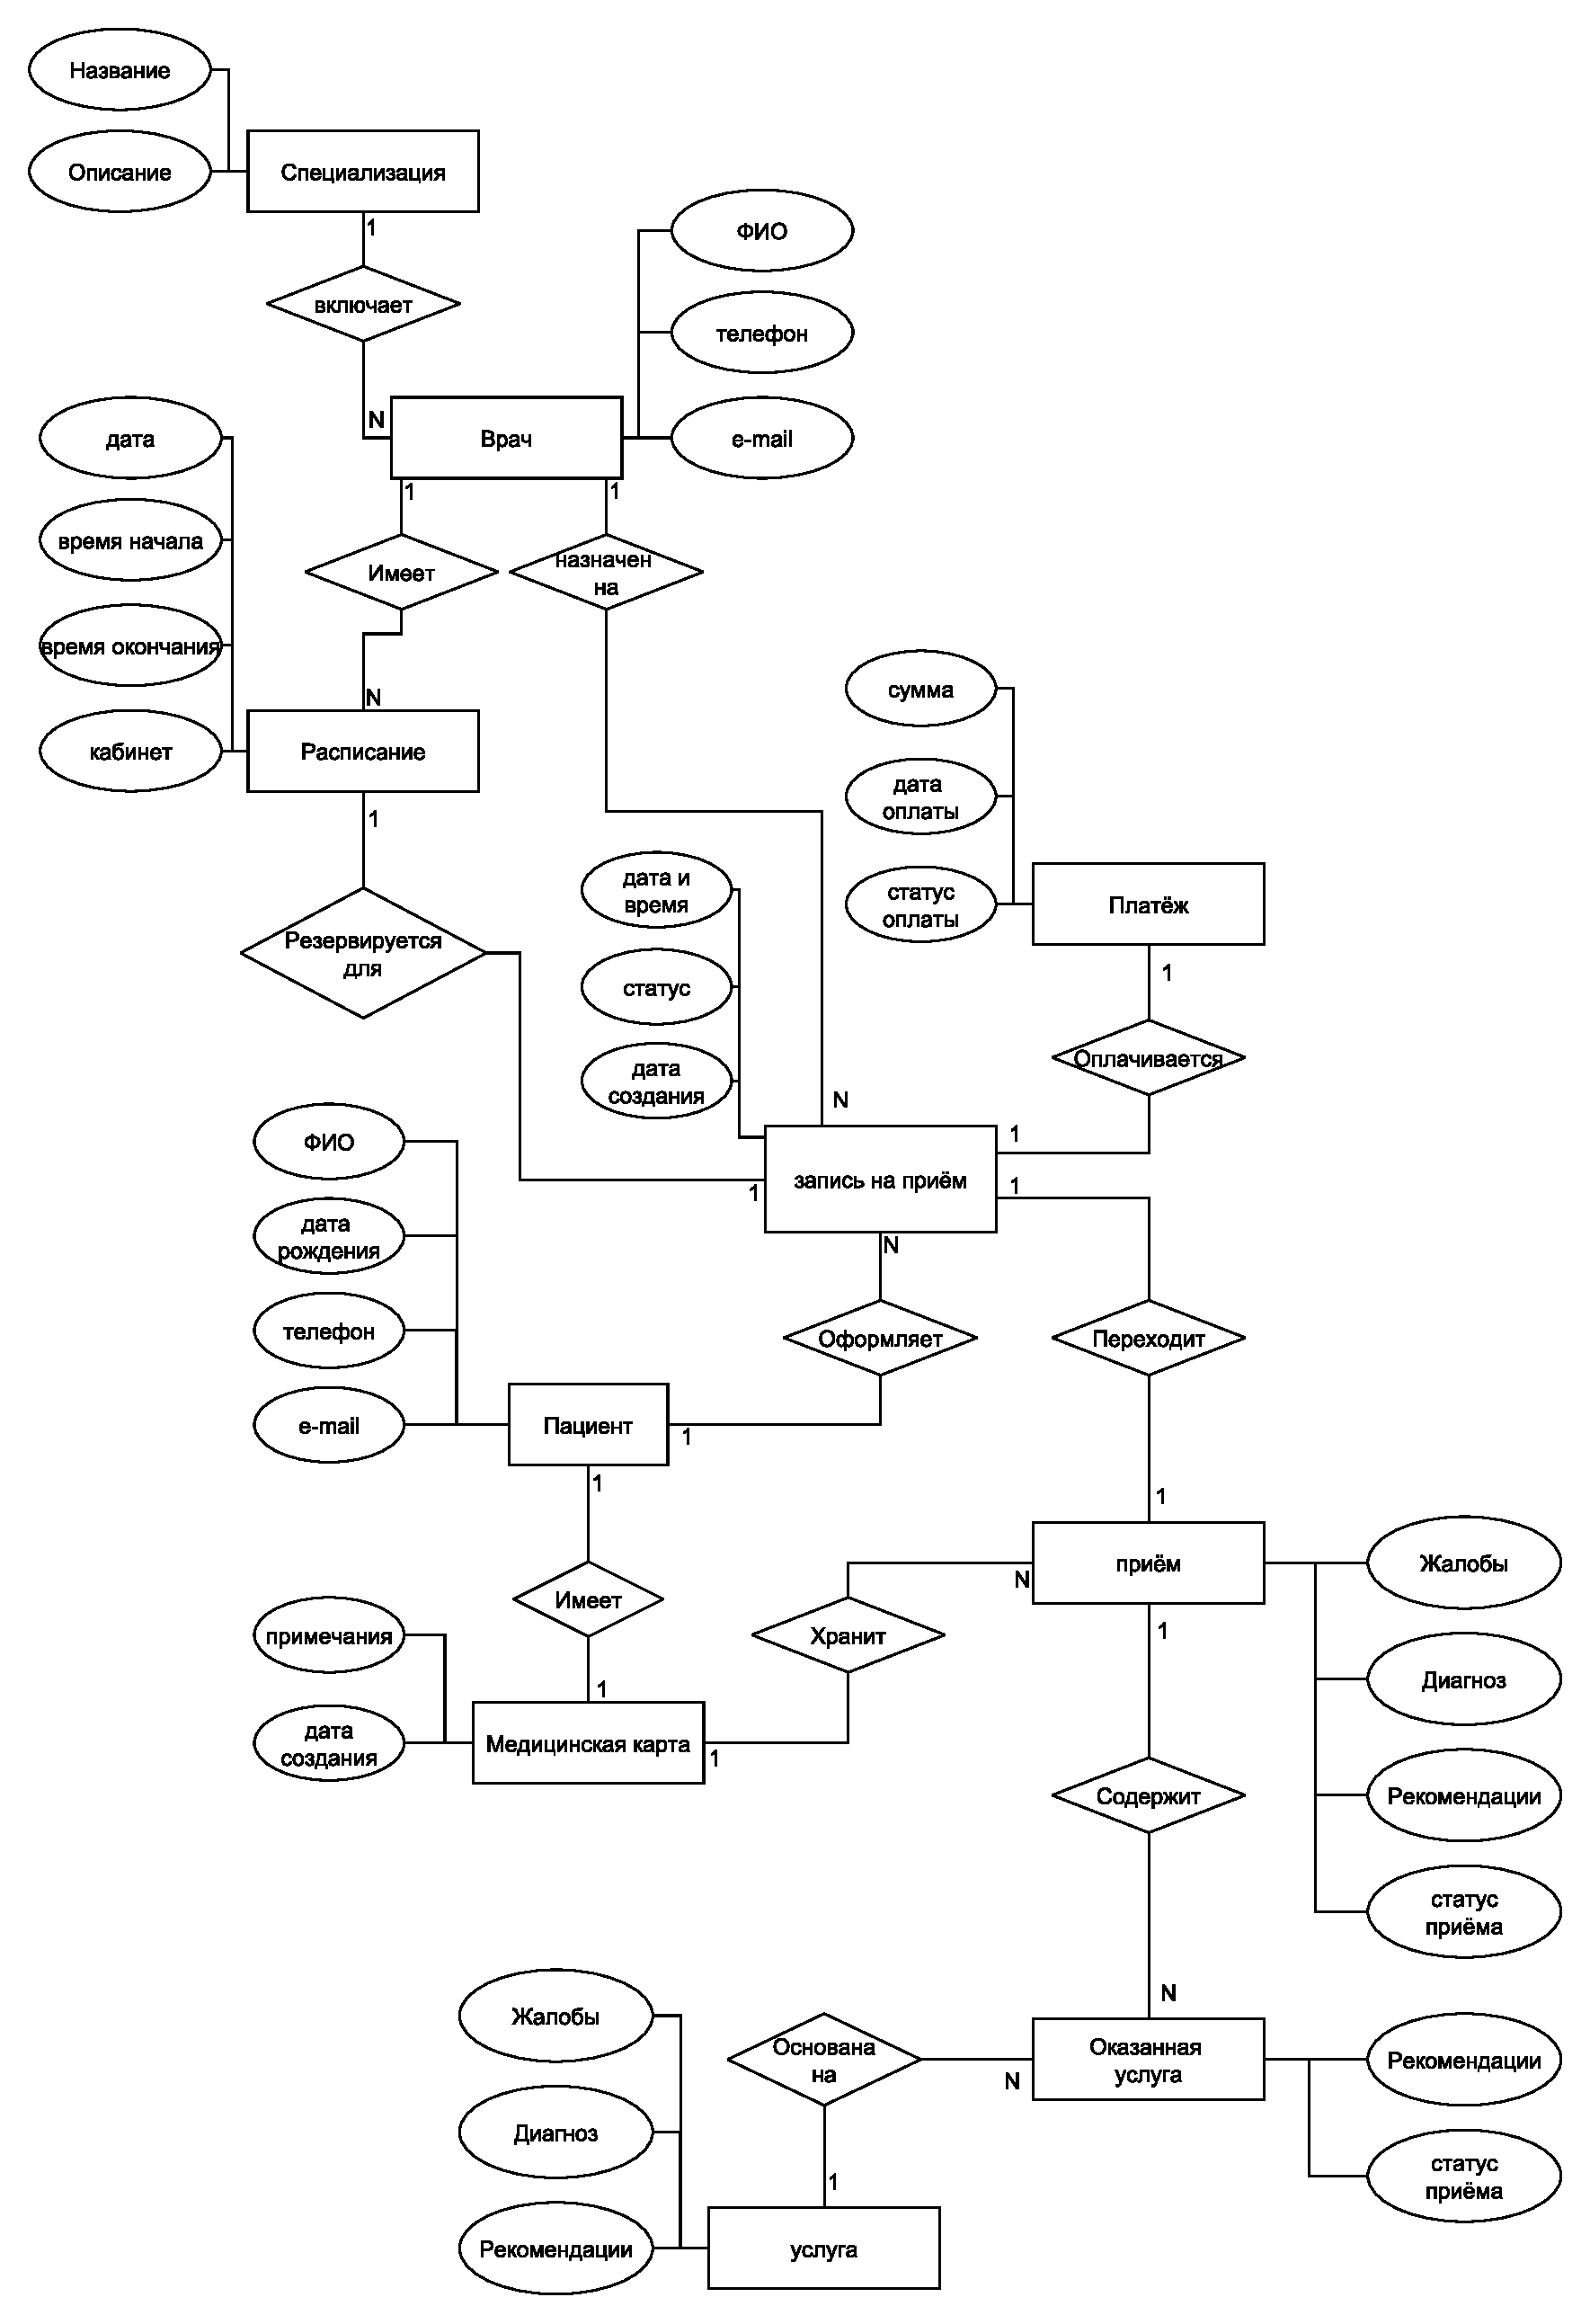
\includegraphics[width=\textwidth,height=0.80\textheight,keepaspectratio]{figures/er-diagram.pdf}
    \caption{ER-диаграмма сущностей базы данных медицинской клиники}
    \label{fig:er-diagram}
\end{figure}

Таким образом, база данных должна обслуживать не только хранение справочной информации, но и сквозной процесс оказания медицинской услуги: от записи пациента на прием до формирования счета и регистрации оплаты.

\section{Формализация ролей}

В системе выделяются три прикладные роли:
\begin{enumerate}
    \item пациент;
    \item администратор;
    \item врач.
\end{enumerate}

Для каждой роли определен собственный набор полномочий. Пациент регистрирует собственную карточку, выбирает врача и услугу, оформляет запись и при необходимости отменяет ее с учетом установленных ограничений. Администратор управляет пользователями, ролями, справочниками и финансовыми операциями, а также сопровождает запись пациента. Врач работает со своим расписанием, проводит прием и фиксирует его результаты.

Полномочия ролей приведены в таблице~\ref{tab:role-responsibilities}.

\begin{table}[ht]
    \centering
    \caption{Роли пользователей и их основные полномочия}
    \label{tab:role-responsibilities}
    \begin{tabular}{|p{3.2cm}|p{5.6cm}|p{4.7cm}|}
        \hline
        Роль & Основные действия & Ограничения \\
        \hline
        Пациент & регистрация собственной карточки, запись и отмена приема, просмотр доступного расписания и прайс-листа & не проводит прием, не регистрирует оплату и не управляет ролями \\
        \hline
        Администратор & управление пользователями, ролями, справочниками, просмотр счетов, регистрация оплат и сопровождение записи пациента & не проводит прием \\
        \hline
        Врач & просмотр своего расписания, завершение приема, фиксация диагноза и оказанных услуг & не регистрирует оплаты и не управляет пользователями \\
        \hline
    \end{tabular}
\end{table}

На рисунке~\ref{fig:use-case} приведена диаграмма вариантов использования, отражающая основные действия ролей в системе.

\begin{figure}[H]
    \centering
    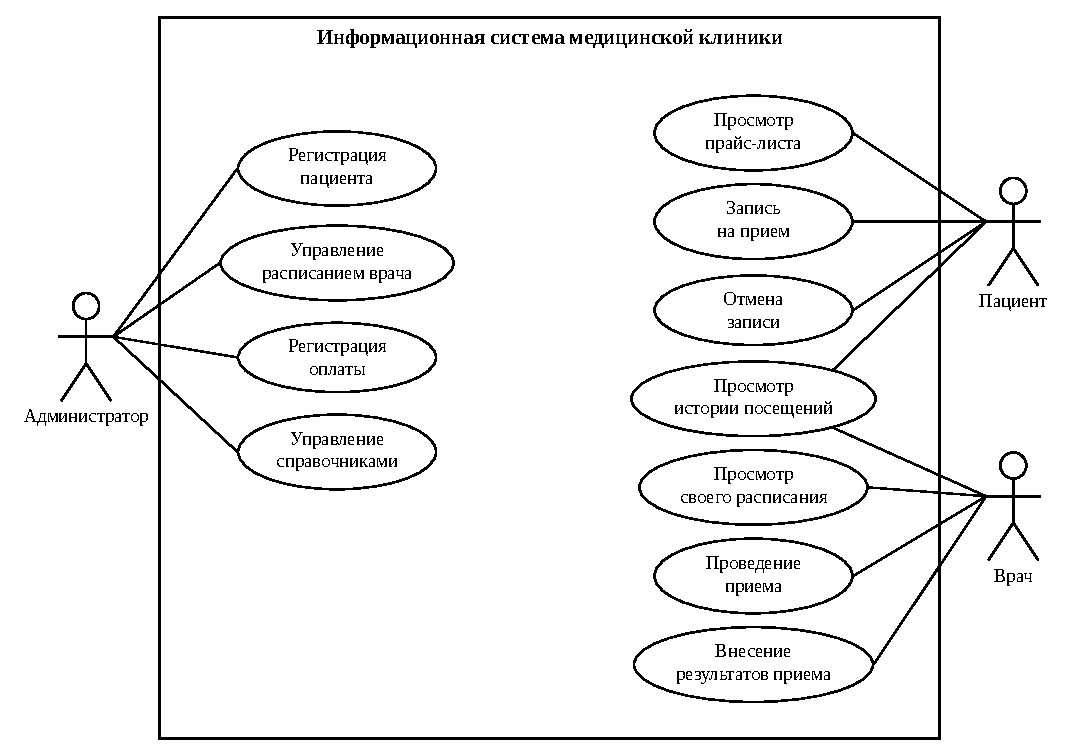
\includegraphics[width=\textwidth,height=0.80\textheight,keepaspectratio]{../diagrams/svg/use-case.pdf}
    \caption{Диаграмма вариантов использования системы медицинской клиники}
    \label{fig:use-case}
\end{figure}

Ролевая структура напрямую влияет на проектирование прикладного API и прав доступа в базе данных, поэтому в конструкторском разделе она будет детализирована уже в терминах ролей PostgreSQL и доступных операций.

\section{Модели данных}

\subsection{Иерархическая модель}

Иерархическая модель данных представляет базу как дерево, в котором каждая запись, кроме корневой, имеет единственного родителя~\cite{date_intro}. Классическим примером является СУБД IBM IMS, разработанная в 1960-х годах для хранения спецификаций космической программы Apollo. Запросы в иерархической модели выполняются навигационным способом --- путем обхода дерева от корня к потомкам.

Для предметной области медицинской клиники такой подход неудобен: пациент, врач, услуга, прием и счет образуют сеть взаимосвязанных сущностей, а не простую древовидную иерархию. Например, один пациент может иметь несколько записей к разным врачам, а один врач --- несколько услуг, что невозможно выразить единственным деревом без дублирования данных.

\subsection{Сетевая модель}

Сетевая модель, формализованная в стандарте CODASYL~\cite{connolly_db}, позволяет записи иметь несколько родительских и дочерних записей, что снимает ограничение иерархической модели. Примером является СУБД IDMS. Навигация по данным осуществляется через явные указатели между записями.

Однако проектирование и сопровождение сетевой модели значительно сложнее, а ее практическое применение в современных прикладных системах ограничено. Изменение структуры связей требует модификации схемы на физическом уровне, что делает модель негибкой для развивающейся системы клиники.

\subsection{Реляционная модель}

Реляционная модель, предложенная Э.\,Ф.~Коддом в 1970 году~\cite{date_intro}, хранит данные в виде отношений (таблиц), связанных между собой ключами. Она естественно поддерживает нормализацию, ограничения целостности, индексы, транзакции, представления, процедуры и триггеры~\cite{connolly_db}. Примеры современных реляционных СУБД: PostgreSQL, MySQL, Oracle Database, Microsoft SQL Server.

Для медицинской клиники это особенно важно, так как требуется одновременно обеспечить целостность расписания, истории цен, приемов, счетов и оплат. Декларативный язык SQL позволяет формулировать сложные запросы без навигационного обхода данных.

\subsection{Многомерная модель}

Многомерная модель ориентирована на аналитические и OLAP-задачи, когда данные рассматриваются как факты и измерения~\cite{connolly_db}. Типичная реализация --- куб данных с осями <<время>>, <<услуга>>, <<врач>>. Примеры СУБД: Microsoft Analysis Services, ClickHouse (колоночное хранение).

Для основной транзакционной системы клиники такая модель непригодна, поскольку операции записи, отмены, проведения приема и оплаты требуют именно оперативной обработки (OLTP) и строгих ограничений целостности, которые многомерные СУБД не обеспечивают.

\subsection{Объектно-ориентированная модель}

Объектно-ориентированная модель хранит данные в виде объектов с инкапсулированными методами и поддерживает наследование~\cite{date_intro}. Примерами являются СУБД ObjectDB и db4o. Такая модель удобна при тесной интеграции с объектными языками программирования.

Однако в рамках данной задачи она не дает достаточных преимуществ перед реляционной моделью. Контроль целостности временных интервалов (EXCLUDE-ограничения), кэширование и конкурентный доступ в курсовом проекте должны опираться на развитые возможности реляционной СУБД, которых объектно-ориентированные СУБД в полной мере не предоставляют.

\subsection{Выбор модели данных}

Сравнение рассмотренных моделей данных по критериям, существенным для разрабатываемой системы, приведено в таблице~\ref{tab:model-comparison}.

\begin{table}[ht]
    \centering
    \caption{Сравнение моделей данных}
    \label{tab:model-comparison}
    \small
    \begin{tabular}{|p{4.0cm}|c|c|c|c|c|}
        \hline
        Критерий & Иерарх. & Сетевая & Реляц. & Многомер. & ОО \\
        \hline
        Связи M:N & Нет & Да & Да & Нет & Да \\
        \hline
        Декларативные запросы & Нет & Нет & Да & Частично & Нет \\
        \hline
        Ограничения целостности & Частично & Частично & Да & Нет & Частично \\
        \hline
        Транзакционная обработка & Частично & Частично & Да & Нет & Да \\
        \hline
        Распространенность СУБД & Низкая & Низкая & Высокая & Средняя & Низкая \\
        \hline
    \end{tabular}
    \normalsize
\end{table}

Наиболее подходящей для разрабатываемой системы является реляционная модель данных. Она обеспечивает естественное выражение связей между сущностями, поддержку нормализации и надежную транзакционную обработку. Выбор PostgreSQL как реляционной СУБД~\cite{postgres_main} дополнительно позволяет использовать перечислимые типы, домены, диапазоны времени, ограничения \texttt{EXCLUDE}~\cite{postgres_constraints}, процедуры и триггеры, что полностью соответствует требованиям задания.

\section{Вывод}

В аналитическом разделе исследована предметная область медицинской клиники, формализована задача разработки базы данных и приложения, выделены сущности и роли пользователей, а также рассмотрены основные модели данных. По результатам анализа обоснован выбор реляционной модели и сформирована основа для конструкторского проектирования базы данных, процедур, ролевой модели и механизмов кэширования.

\clearpage

% Конструкторский раздел
\chapter{Конструкторский раздел}

В данном разделе разработана структура базы данных медицинской клиники, определены ограничения целостности, процедуры, триггеры, роли и правила кэширования.

\section{Схема проектируемой базы данных}

База данных разделена на логические схемы безопасности, справочников, расписания, медицинских и финансовых данных. Такое разбиение позволяет отделить подсистему безопасности от справочных, операционных и финансовых данных. ER-диаграмма сущностей приведена в аналитическом разделе (рисунок~\ref{fig:er-diagram}).

Схема проектируемой базы данных приведена на рисунке~\ref{fig:db-diagram}.

\clearpage
\begin{figure}[H]
    \centering
    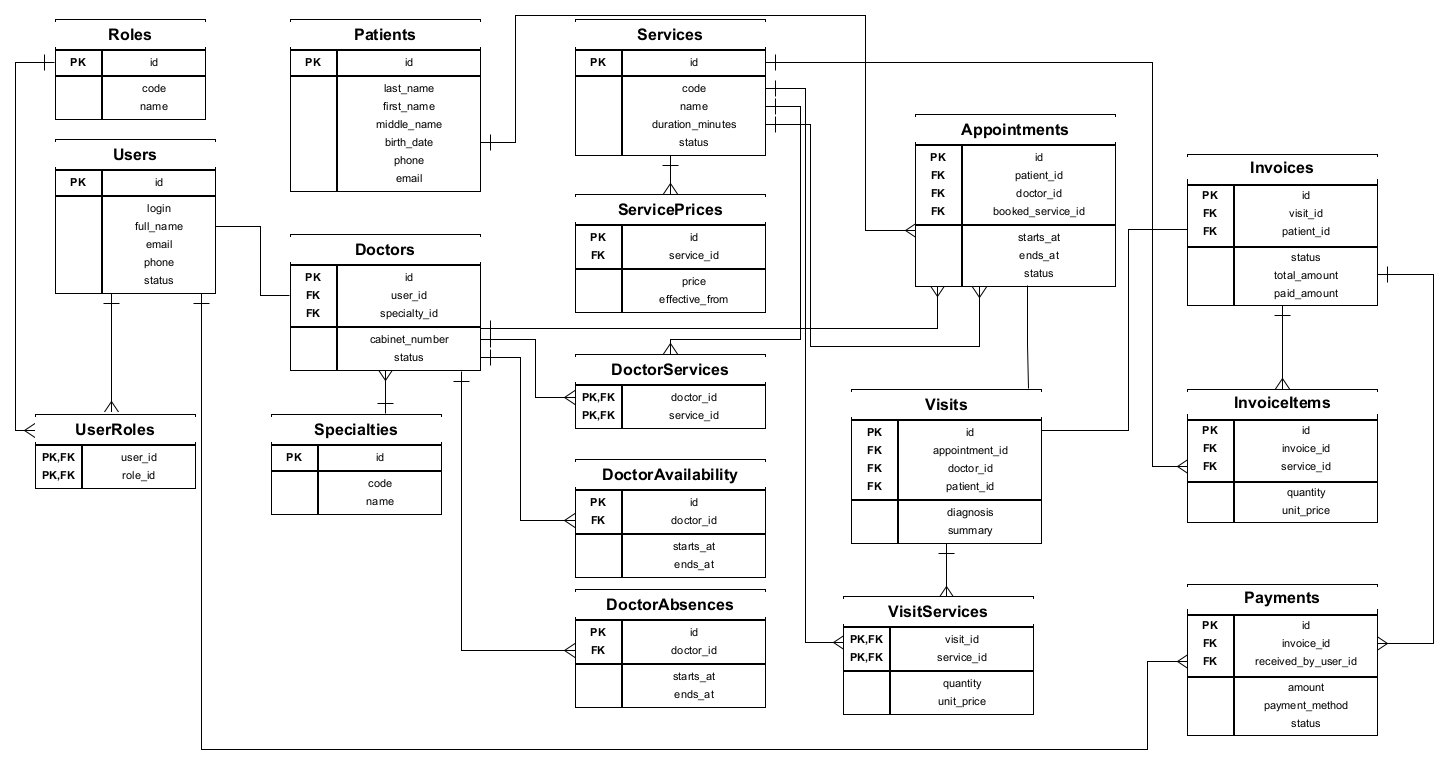
\includegraphics[width=\textwidth,height=1.1\textheight,keepaspectratio]{../diagrams/svg/Db_diagr.png}
    \caption{Схема проектируемой базы данных медицинской клиники}
    \label{fig:db-diagram}
\end{figure}

\clearpage
\section{Описание сущностей}

В разработанной базе данных сущности сгруппированы по функциональным схемам PostgreSQL. Такое разбиение соответствует фактической реализации проекта и позволяет разделить подсистемы безопасности, справочников, медицинских данных, расписания и расчетов.

\subsection{Подсистема безопасности}

Таблица \texttt{security.roles} хранит перечень ролей базы данных прикладного уровня. Для каждой роли задаются уникальные атрибуты \texttt{code} и \texttt{name}, позволяющие однозначно идентифицировать назначение роли.

Таблица \texttt{security.users} описывает учетные записи пользователей системы. В ней хранятся логин, хэш пароля, полное имя, контактные данные и статус учетной записи. Данная таблица используется для учетных записей прикладных пользователей системы: пациента, администратора и врача, а также для фиксации автора операций записи, отмены и приема оплаты.

Таблица \texttt{user\_roles} задает связь <<пользователь -- роль>>. Через нее одному пользователю могут быть назначены несколько ролей.

\subsection{Справочные сущности}

Таблица \texttt{catalog.specialties} содержит справочник врачебных специальностей. Записи этой таблицы используются при описании врачей и при группировке расписания и отчетов по профилю врача.

Таблица \texttt{catalog.services} описывает медицинские услуги, доступные в клинике. Для услуги хранятся код, наименование, описание, нормативная длительность приема и статус доступности. Именно эта сущность используется как при планировании записи, так и при формировании фактически оказанных услуг.

Таблица \texttt{catalog.service\_prices} хранит историю стоимости услуг. Для каждой цены задаются дата начала действия, дата окончания действия и стоимость в валюте \texttt{RUB}. Таким образом обеспечивается возможность расчета стоимости услуг с учетом периода действия прайс-листа.

\subsection{Медицинские сущности}

Таблица \texttt{medical.patients} хранит сведения о пациентах: фамилию, имя, отчество, дату рождения, контактные данные, номер страхового полиса и статус записи о пациенте. Эта таблица используется при записи на прием, ведении истории обращений и формировании счетов.

Таблица \texttt{medical.doctors} описывает врачей клиники. Каждая запись связана с учетной записью пользователя и со специальностью, а также содержит номер кабинета и статус врача. Связь с таблицей \texttt{security.users} имеет характер один-к-одному, что позволяет разделить сведения о сотруднике и сведения о доступе в систему.

Таблица \texttt{doctor\_services} реализует связь многие-ко-многим между врачами и услугами. Она определяет, какие услуги конкретный врач имеет право выполнять.

Таблица \texttt{medical.visits} фиксирует факт проведенного приема. Она связана с конкретной записью на прием, а также содержит ссылки на врача и пациента, диагноз и краткое описание результата приема.

Таблица \texttt{medical.visit\_services} содержит перечень услуг, фактически оказанных в рамках приема. Для каждой позиции сохраняются количество, цена за единицу и итоговая стоимость строки, что позволяет далее автоматически формировать счет.

\subsection{Сущности расписания и записи}

Таблица \texttt{scheduling.doctor\_availability} описывает интервалы доступности врача для записи. Для каждого интервала задаются начало и окончание периода, длительность слота и признак активности расписания.

Таблица \texttt{scheduling.doctor\_absences} хранит интервалы отсутствия врача с указанием причины. Эти данные используются при контроле доступности времени записи и при проверке возможности проведения приема.

Таблица \texttt{scheduling.appointments} описывает записи пациентов на прием. Она связывает пациента, врача и планируемую услугу, хранит время начала и окончания приема, статус записи, служебное примечание, причину отмены, а также ссылки на пользователей, создавших или отменивших запись. Данная таблица является центральной сущностью операционного контура базы данных.

\subsection{Финансовые сущности}

Таблица \texttt{billing.invoices} хранит счета, сформированные по результатам проведенного приема. Каждый счет связан с одним приемом и пациентом, а также содержит итоговую сумму, сумму оплаты и текущий статус расчета.

Таблица \texttt{billing.invoice\_items} содержит позиции счета. Каждая позиция связывает счет с конкретной услугой и хранит количество, цену и стоимость строки. Содержимое данной таблицы формируется на основе таблицы \texttt{medical.visit\_services}.

Таблица \texttt{billing.payments} хранит сведения об оплатах по счетам. Для каждой оплаты фиксируются сумма, способ оплаты, статус, внешний идентификатор операции и пользователь, зарегистрировавший оплату.

Таким образом, основная цепочка предметной области в реализованной базе данных выглядит следующим образом: пациент или администратор формирует запись пациента к врачу на услугу, проведенный прием порождает запись о визите и перечень оказанных услуг, после чего на их основе формируется счет и регистрируются оплаты.

\section{Ограничения целостности}

\subsection{Домены и перечислимые типы}

В схеме используются домены PostgreSQL \texttt{security.email\_address} и \texttt{security.phone\_number}. Они задают единые правила проверки e-mail и телефона и позволяют централизованно использовать один формат в таблицах пользователей и пациентов.

Для описания состояний сущностей применяются перечислимые типы PostgreSQL. Это исключает появление произвольных строковых значений и фиксирует допустимые переходы между состояниями. Модель статусов приведена в таблице~\ref{tab:status-model}.

\begin{table}[H]
    \centering
    \caption{Модель статусов и перечислимых типов PostgreSQL}
    \label{tab:status-model}
    \footnotesize
    \renewcommand{\arraystretch}{1.1}
    \setlength{\tabcolsep}{4pt}
    \begin{tabularx}{\textwidth}{|>{\raggedright\arraybackslash}p{2.85cm}|>{\raggedright\arraybackslash}p{4.15cm}|>{\raggedright\arraybackslash}X|}
        \hline
        Сущность & Тип PostgreSQL & Допустимые значения \tabularnewline
        \hline
        Пользователь & \begin{tabular}[t]{@{}l@{}}{\scriptsize\texttt{security.}}\tabularnewline{\scriptsize\texttt{user\_status}}\end{tabular} & active, inactive, archived \tabularnewline
        \hline
        Пациент & \begin{tabular}[t]{@{}l@{}}{\scriptsize\texttt{medical.}}\tabularnewline{\scriptsize\texttt{patient\_status}}\end{tabular} & active, inactive, archived \tabularnewline
        \hline
        Врач & \begin{tabular}[t]{@{}l@{}}{\scriptsize\texttt{medical.}}\tabularnewline{\scriptsize\texttt{doctor\_status}}\end{tabular} & active, inactive, archived \tabularnewline
        \hline
        Услуга & \begin{tabular}[t]{@{}l@{}}{\scriptsize\texttt{catalog.}}\tabularnewline{\scriptsize\texttt{service\_status}}\end{tabular} & active, inactive, archived \tabularnewline
        \hline
        Запись на прием & \begin{tabular}[t]{@{}l@{}}{\scriptsize\texttt{scheduling.}}\tabularnewline{\scriptsize\texttt{appointment\_status}}\end{tabular} & \begin{tabular}[t]{@{}l@{}}booked, cancelled,\tabularnewline completed\end{tabular} \tabularnewline
        \hline
        Счет & \begin{tabular}[t]{@{}l@{}}{\scriptsize\texttt{billing.}}\tabularnewline{\scriptsize\texttt{invoice\_status}}\end{tabular} & \begin{tabular}[t]{@{}l@{}}issued, partially\_paid,\tabularnewline paid, cancelled\end{tabular} \tabularnewline
        \hline
        Оплата & \begin{tabular}[t]{@{}l@{}}{\scriptsize\texttt{billing.}}\tabularnewline{\scriptsize\texttt{payment\_status}}\end{tabular} & completed, cancelled \tabularnewline
        \hline
    \end{tabularx}
\end{table}
\normalsize

\subsection{Ключи и связи многие-ко-многим}

Во всех основных таблицах в качестве первичных ключей используются значения типа \texttt{UUID}. Такой подход позволяет формировать идентификаторы независимо от конкретного клиента. Он также не раскрывает информацию о количестве записей.

Ссылочная целостность обеспечивается внешними ключами. Связи многие-ко-многим реализованы тремя промежуточными таблицами:
\begin{itemize}
    \item \texttt{doctor\_services} --- связь <<врач -- услуга>>;
    \item \texttt{visit\_services} --- связь <<прием -- оказанная услуга>>;
    \item \texttt{user\_roles} --- связь <<пользователь -- роль>>.
\end{itemize}

\subsection{Ограничения времени и запрет конфликтов}

Для таблиц истории цен, доступности врача, отсутствий врача и записей на прием используются диапазоны типа \texttt{TSTZRANGE}. Это позволяет единообразно хранить временные интервалы и применять к ним ограничения пересечения.

Для предотвращения двойной записи у одного врача используется ограничение \texttt{EXCLUDE}. Оно запрещает пересечение интервалов времени у активных записей и тем самым обеспечивает бесконфликтную работу в многопользовательском режиме.

\subsection{Доказательство 3НФ}

Спроектированная база данных находится в третьей нормальной форме по следующим причинам:
\begin{enumerate}
    \item все таблицы имеют первичный ключ, а их атрибуты являются атомарными;
    \item в таблицах со составным ключом, таких как \texttt{doctor\_services}, \texttt{visit\_services} и \texttt{user\_roles}, неключевые атрибуты не зависят от части ключа;
    \item транзитивные зависимости устранены выделением самостоятельных сущностей для ролей, специальностей, истории цен, оказанных услуг, счетов и оплат.
\end{enumerate}

Следовательно, каждый неключевой атрибут зависит только от ключа, от полного ключа и ни от чего, кроме ключа, что и соответствует требованиям 3НФ.

\section{Процедуры, функции и триггеры}

На уровне базы данных реализованы процедуры делового регламента и вспомогательные функции. Они обеспечивают контроль прав, выбор актуальной цены, пересчет счета и автоматическое обновление служебных полей.

\subsection{Вспомогательные функции}

Функция \texttt{set\_updated\_at} используется триггерами для автоматического обновления поля \texttt{updated\_at} перед изменением записи. Схема функции приведена на рисунке~\ref{fig:yed-set-updated-at}.

\begin{figure}[H]
    \centering
    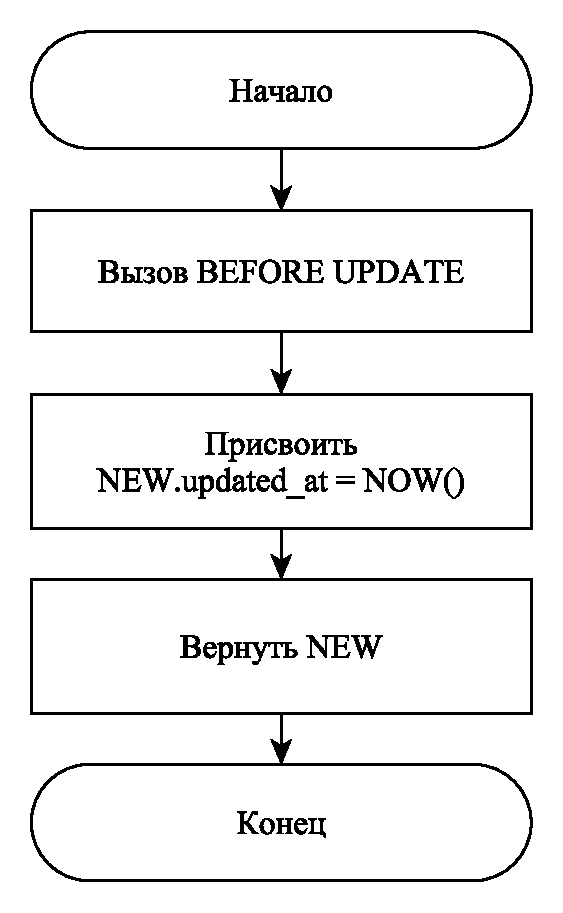
\includegraphics[width=0.40\textwidth]{figures/yed_set_updated_at.pdf}
    \caption{Схема функции \texttt{set\_updated\_at}}
    \label{fig:yed-set-updated-at}
\end{figure}

Функция \texttt{has\_role} проверяет наличие прикладной роли у пользователя. Схема функции приведена на рисунке~\ref{fig:yed-has-role}.

\begin{figure}[H]
    \centering
    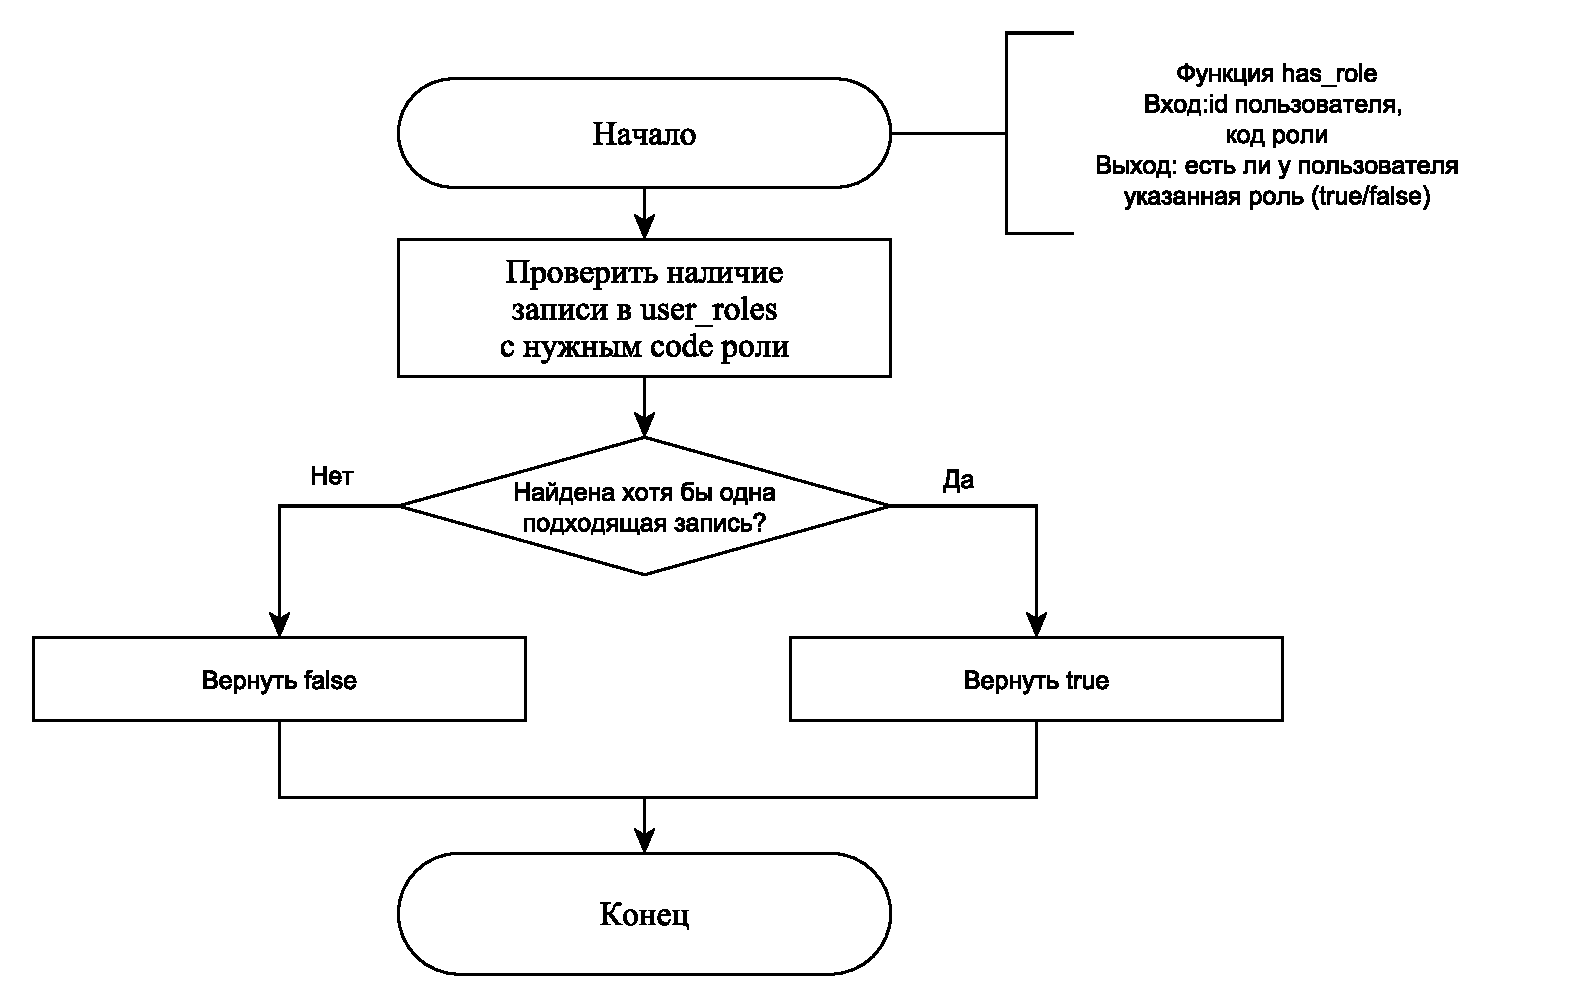
\includegraphics[width=0.74\textwidth]{figures/yed_has_role.pdf}
    \caption{Схема функции \texttt{has\_role}}
    \label{fig:yed-has-role}
\end{figure}

Функция \texttt{get\_service\_price} выбирает актуальную цену услуги на заданный момент времени. Схема функции приведена на рисунке~\ref{fig:yed-get-service-price}.

\begin{figure}[H]
    \centering
    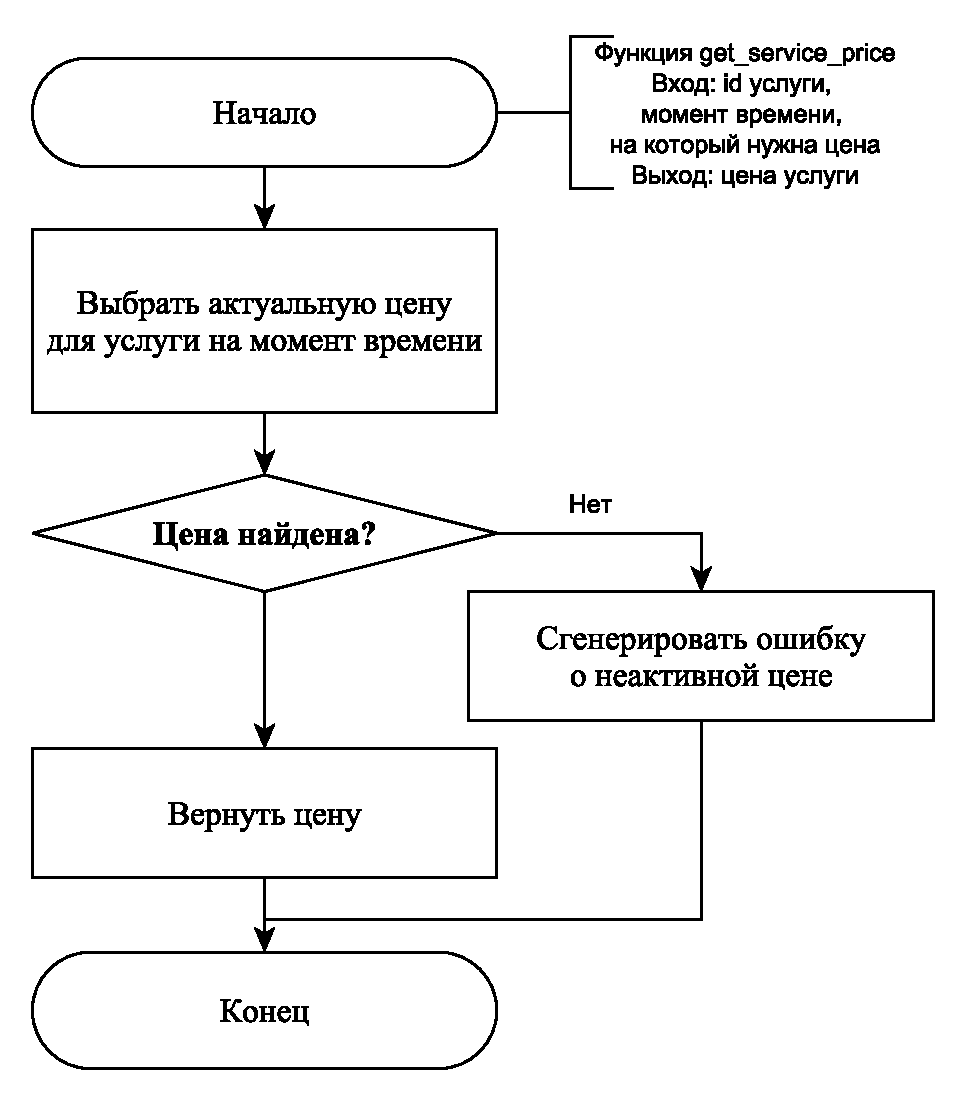
\includegraphics[width=0.6\textwidth]{figures/yed_get_service_price.pdf}
    \caption{Схема функции \texttt{get\_service\_price}}
    \label{fig:yed-get-service-price}
\end{figure}

\subsection{Процедуры делового регламента}

Схема процедуры записи на прием приведена на рисунке~\ref{fig:design-book-appointment}.

Функция \texttt{book\_appointment} проверяет время начала приема, активность пациента и врача, закрепление услуги за врачом и активность самой услуги. Затем вычисляется время окончания приема, проверяются интервал доступности врача и отсутствие записи о его отсутствии. Конфликт по времени дополнительно предотвращается ограничением \texttt{EXCLUDE} при вставке записи.

\begin{figure}[H]
    \centering
    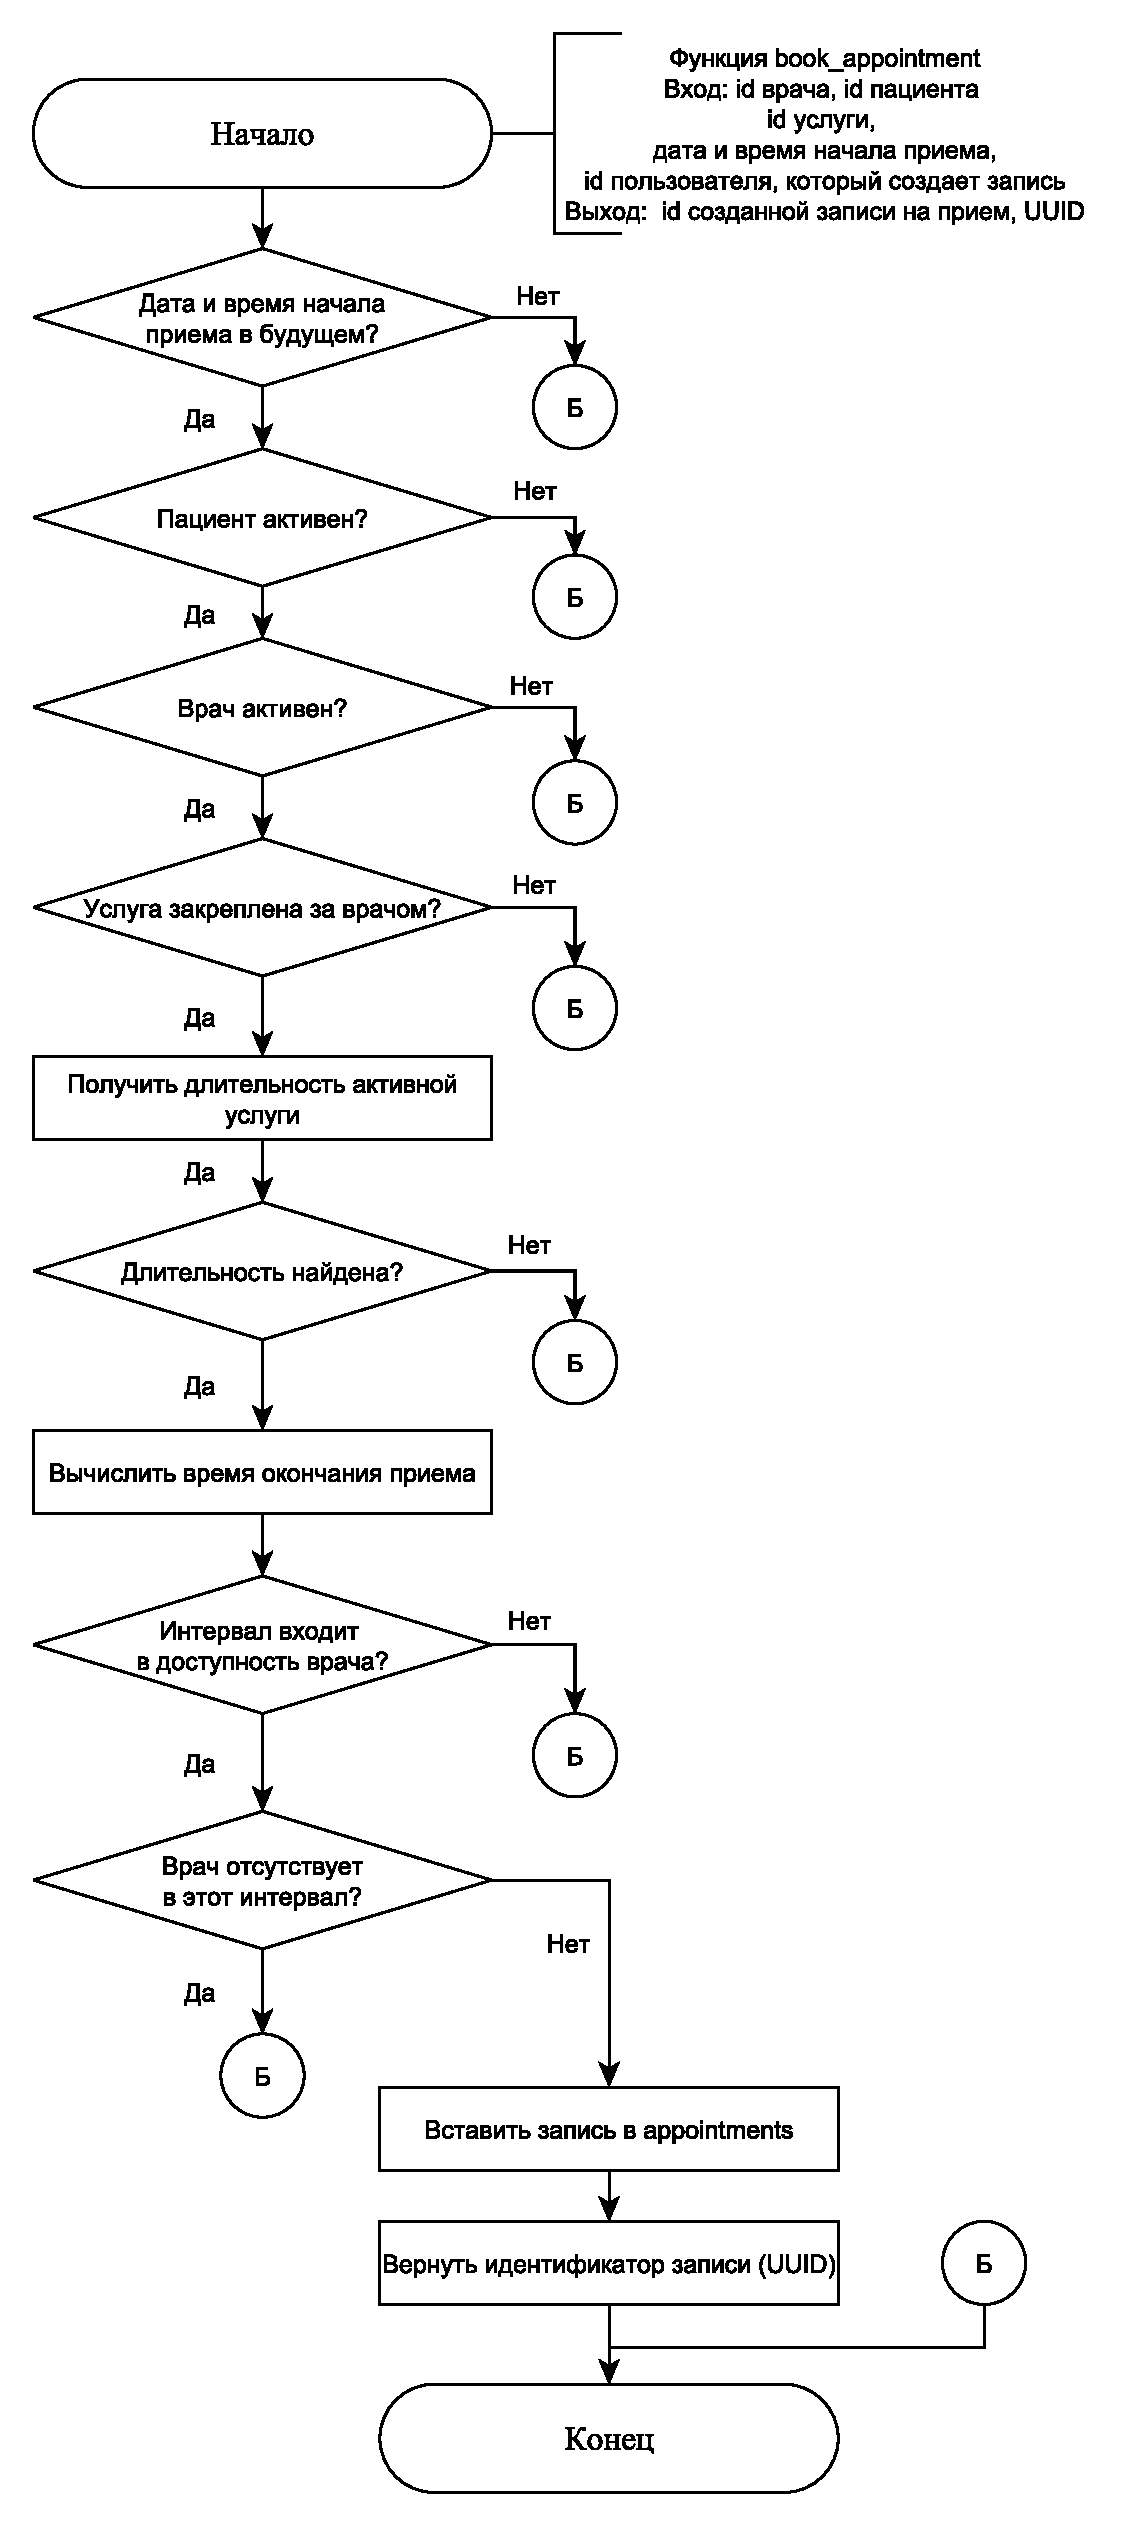
\includegraphics[height=0.90\textheight,keepaspectratio]{figures/yed_book_appointment.pdf}
    \caption{Схема функции \texttt{book\_appointment}}
    \label{fig:design-book-appointment}
\end{figure}

\newpage

Схема отмены записи приведена на рисунке~\ref{fig:design-cancel-appointment}.

Функция \texttt{cancel\_appointment} блокирует строку записи и проверяет ее состояние. Для пациента дополнительно действует правило отмены не позднее чем за 24 часа до приема, тогда как администратор может выполнить отмену без этого ограничения.

\begin{figure}[H]
    \centering
    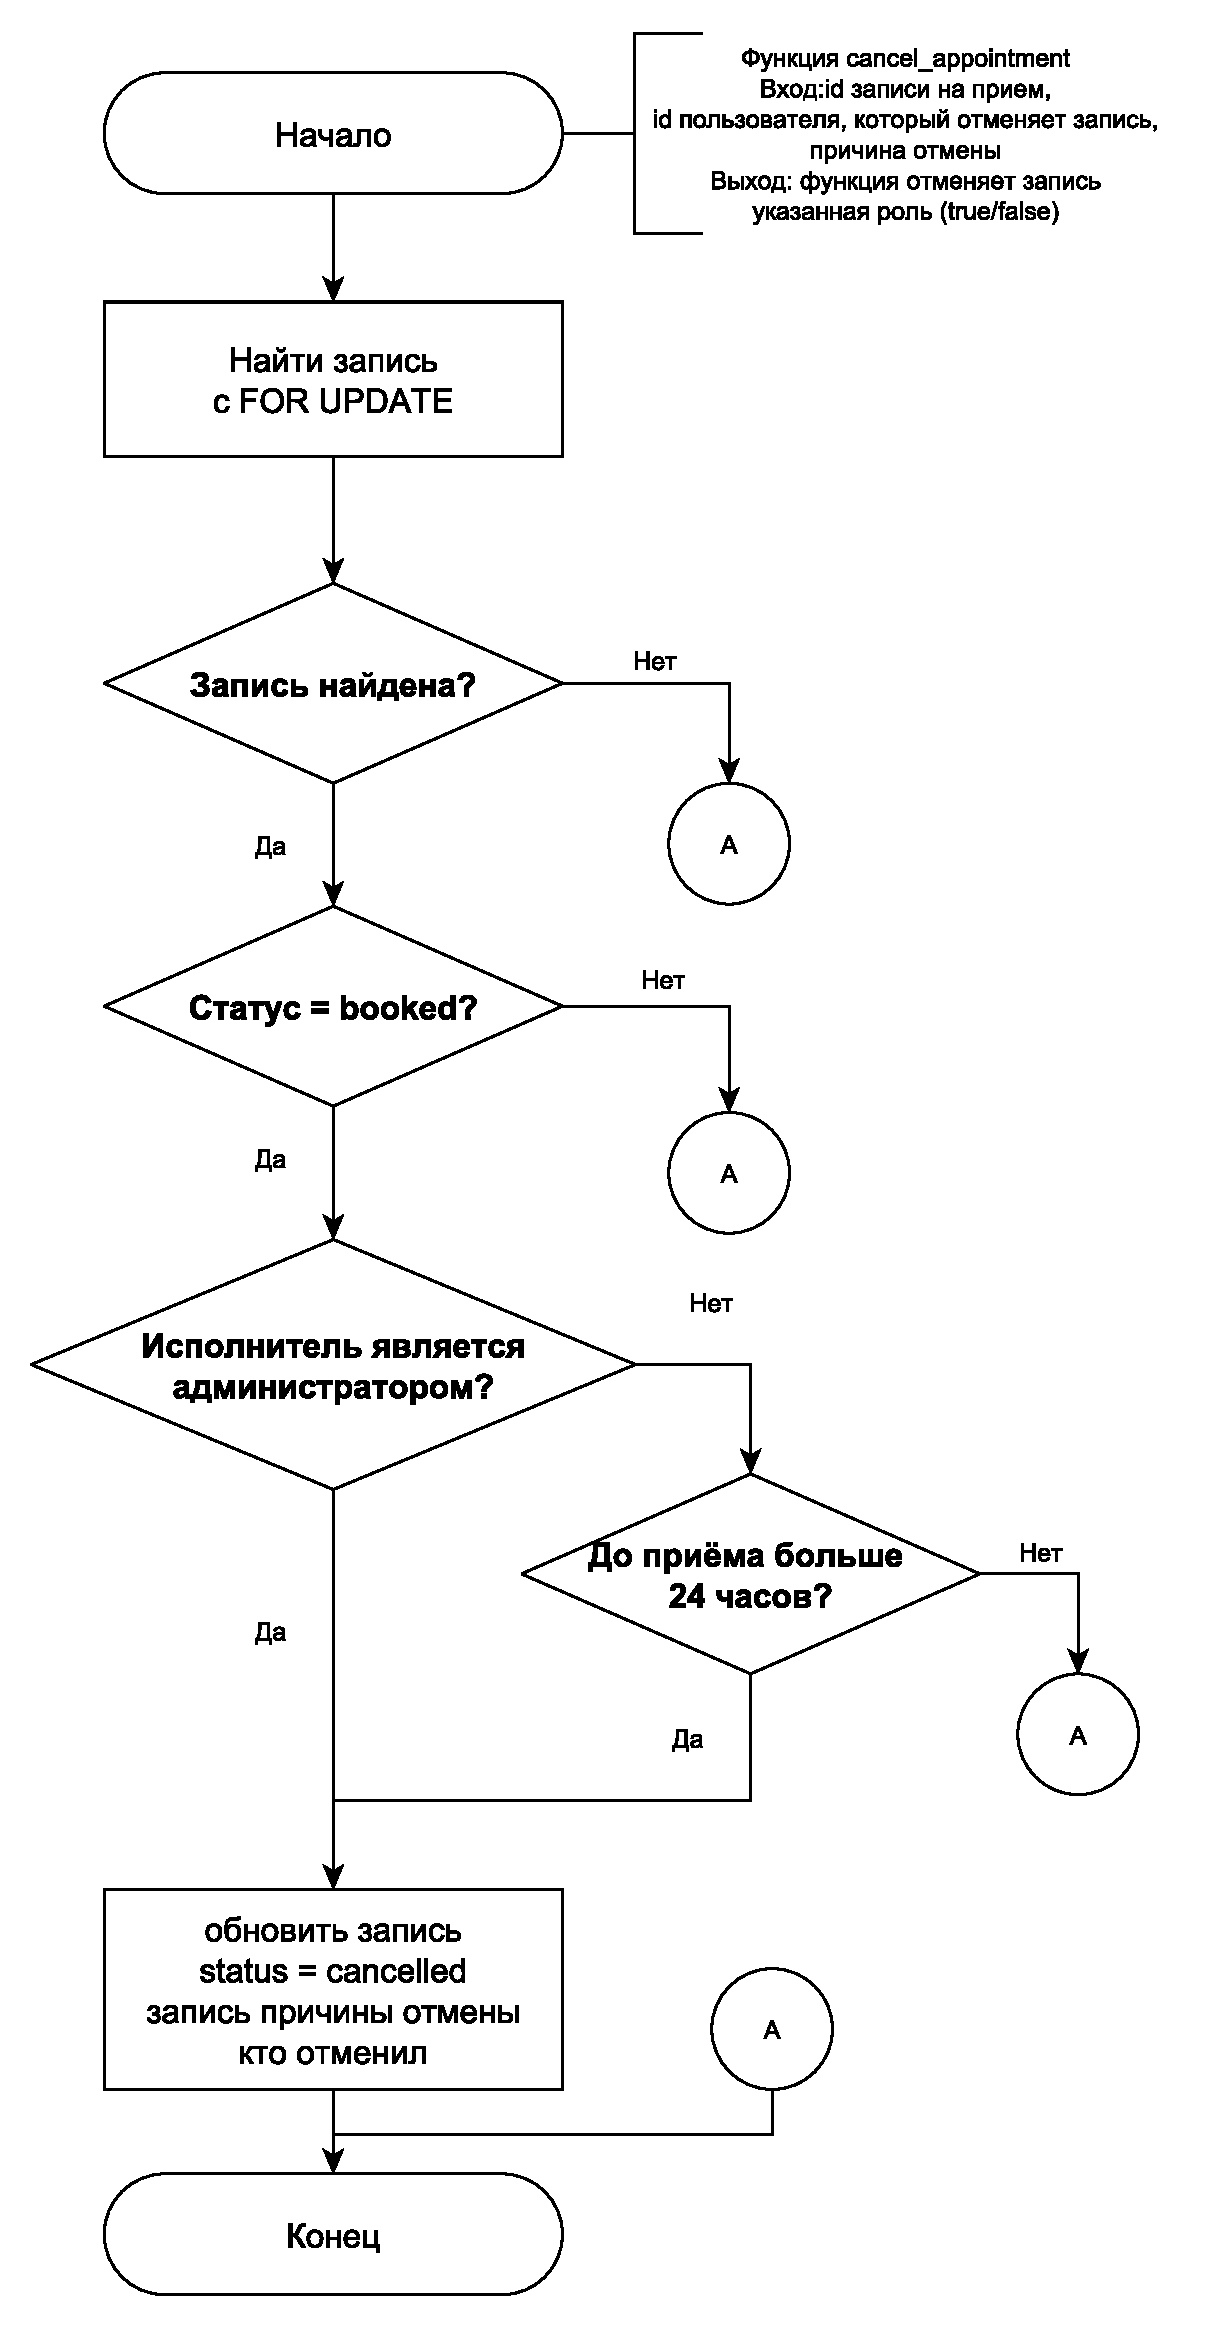
\includegraphics[width=0.70\textwidth]{figures/yed_cancel_appointment.pdf}
    \caption{Схема функции \texttt{cancel\_appointment}}
    \label{fig:design-cancel-appointment}
\end{figure}

\newpage

Схема функции проведения приема приведена на рисунке~\ref{fig:design-complete-visit}.

Функция \texttt{complete\_visit} создает запись о визите и фиксирует оказанные услуги. Если список оказанных услуг пуст, в \texttt{visit\_services} заносится забронированная услуга; иначе обрабатывается переданный список услуг. Затем формируются счет и строки счета, запись на прием переводится в состояние \texttt{completed}, после чего вызывается \texttt{refresh\_invoice\_state}.

\begin{figure}[H]
    \centering
    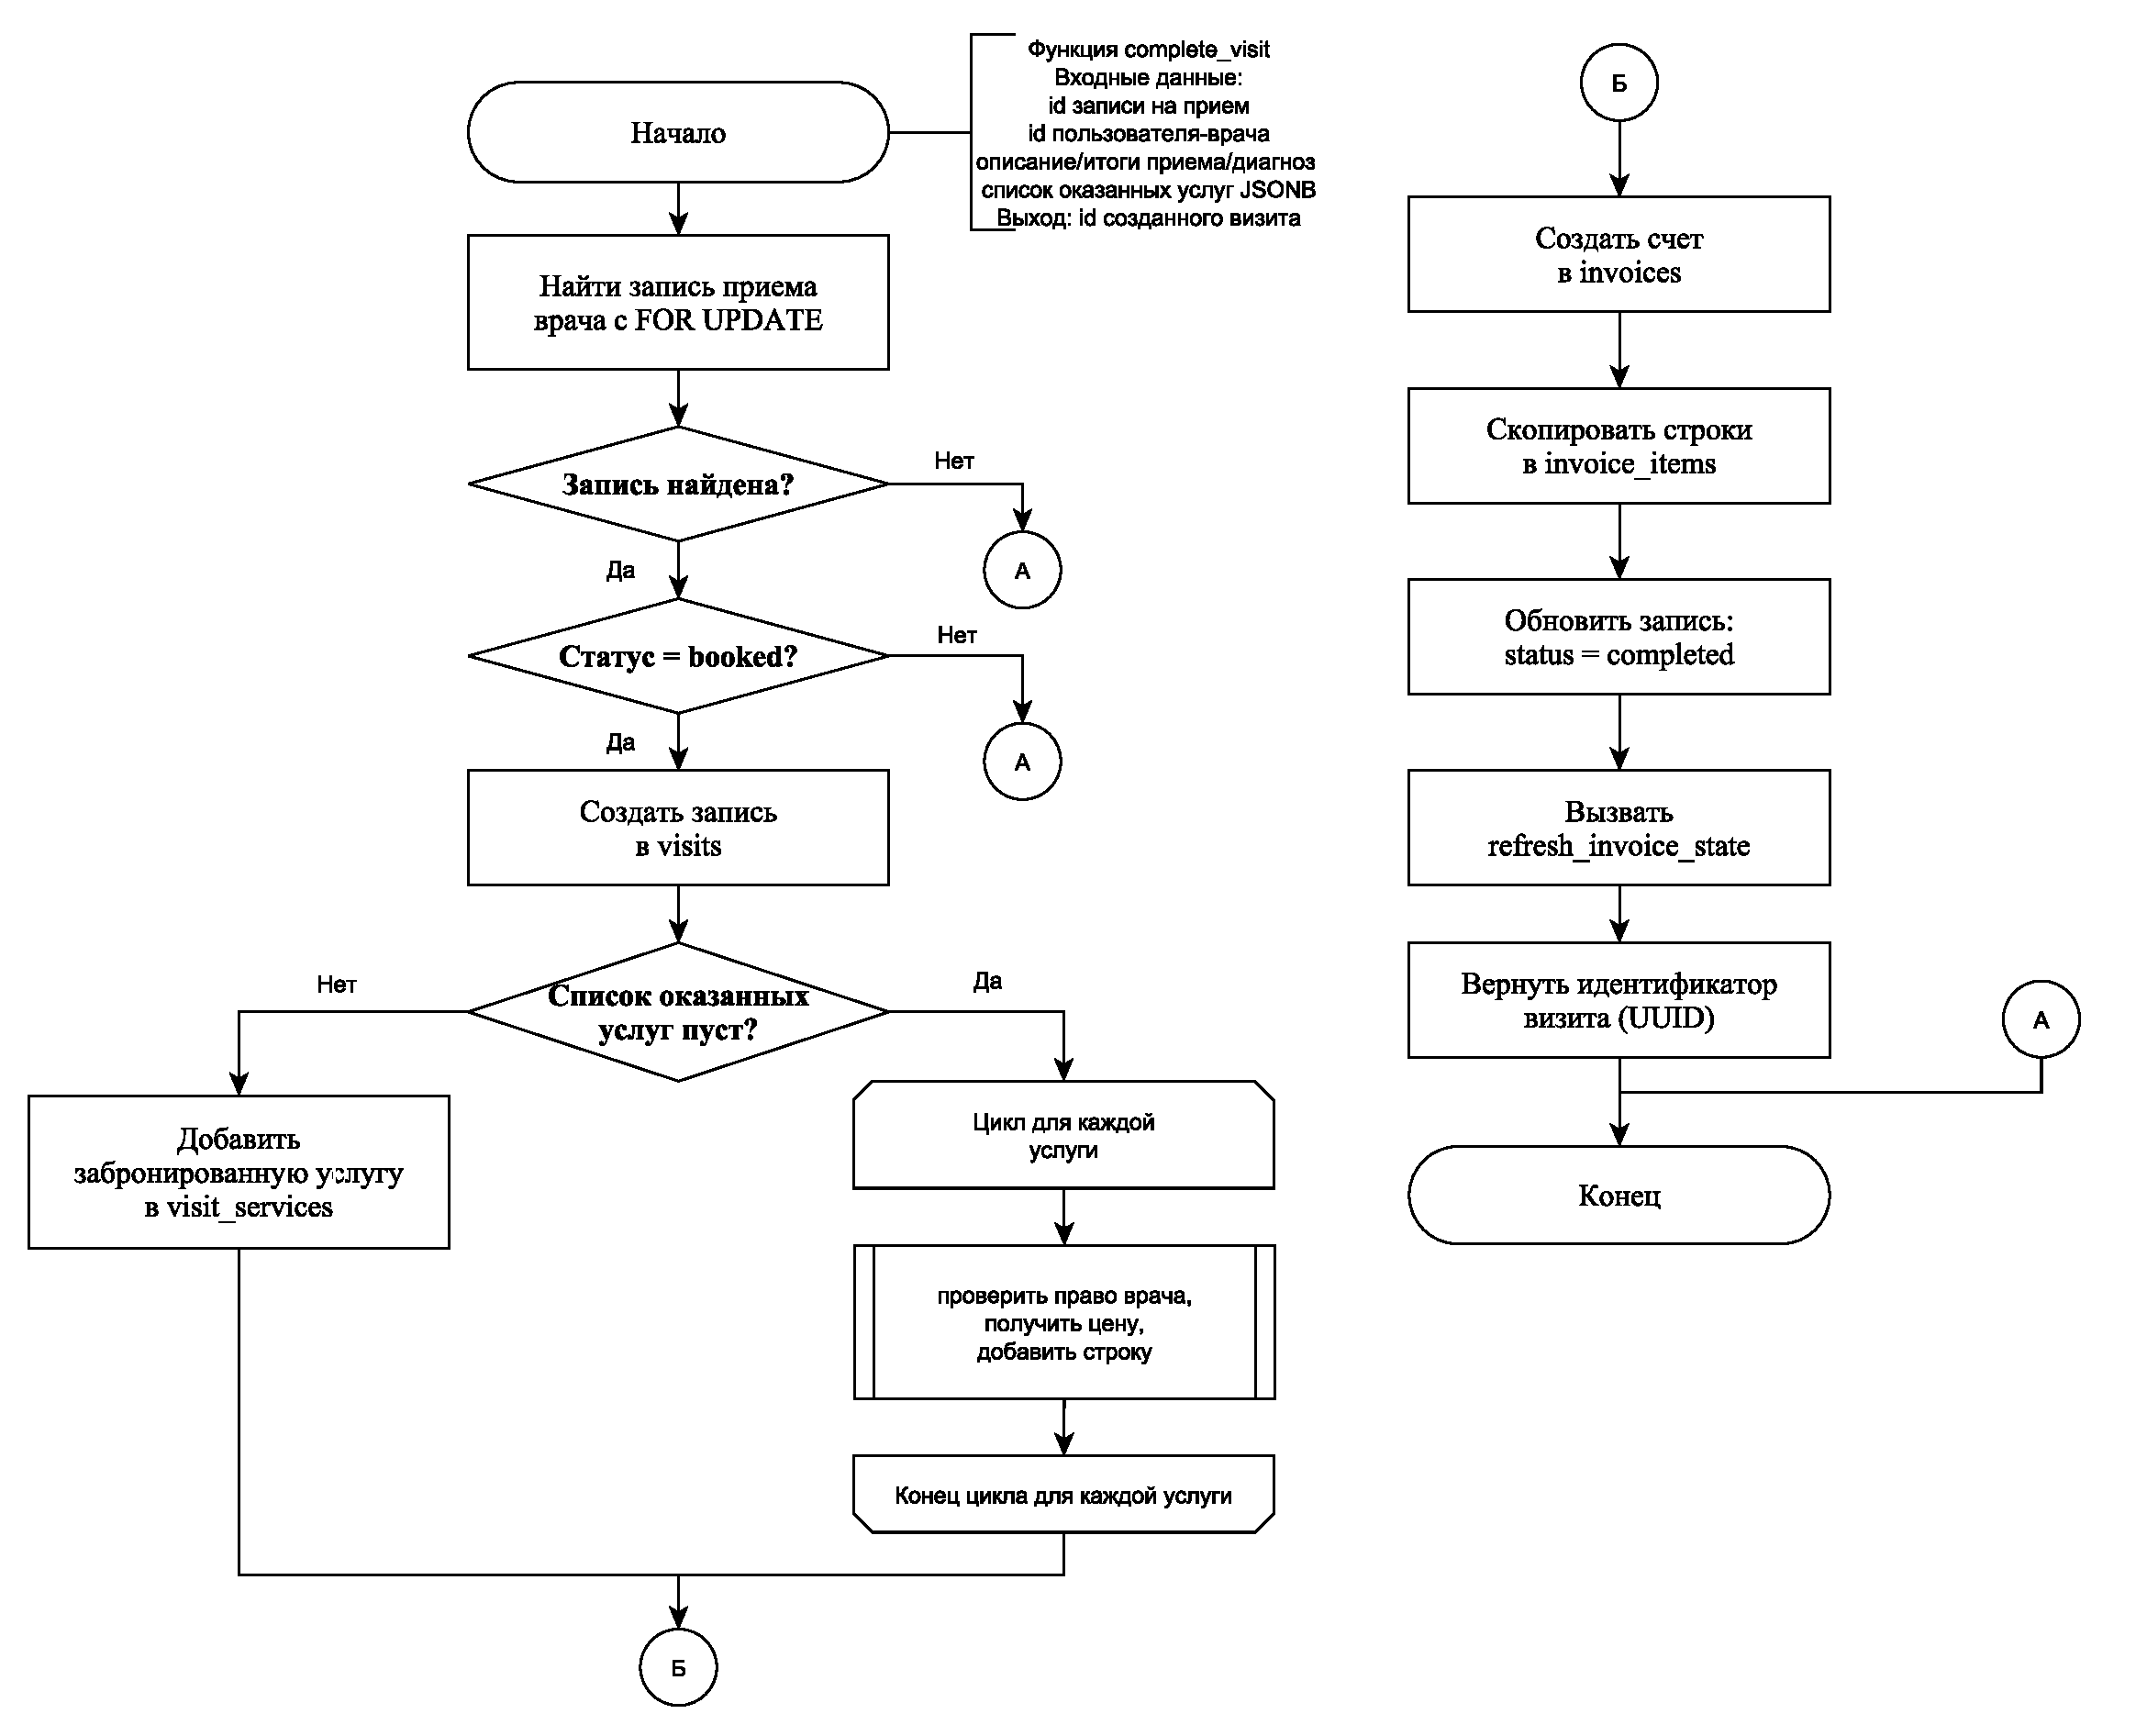
\includegraphics[width=0.8\textwidth]{figures/yed_complete_visit.pdf}
    \caption{Схема функции \texttt{complete\_visit}}
    \label{fig:design-complete-visit}
\end{figure}

\newpage

Схема регистрации оплаты приведена на рисунке~\ref{fig:design-register-payment}.

Функция \texttt{register\_payment} создает запись об оплате. Затем инициируется пересчет состояния счета.

\begin{figure}[H]
    \centering
    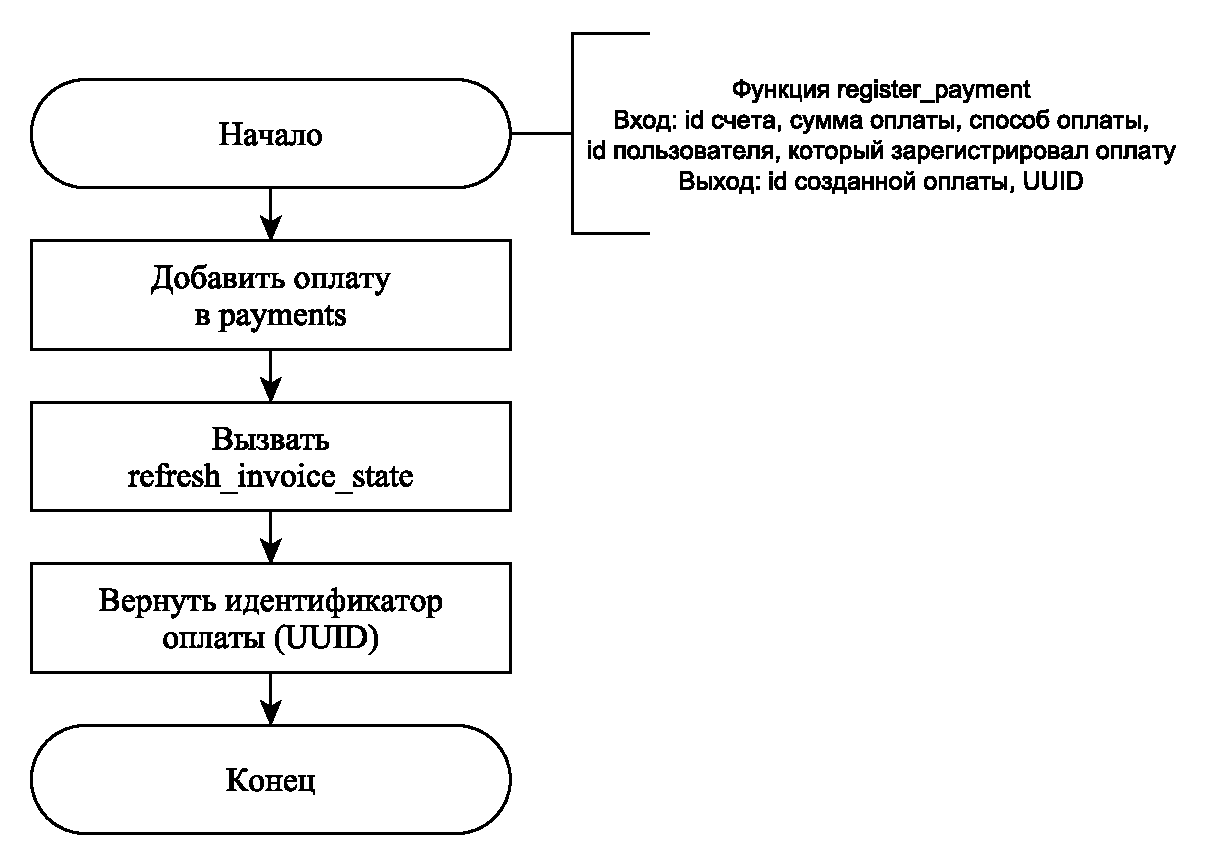
\includegraphics[width=0.55\textwidth]{figures/yed_register_payment.pdf}
    \caption{Схема функции \texttt{register\_payment}}
    \label{fig:design-register-payment}
\end{figure}

\subsection{Функции пересчета счета и триггеры}

Схема функции \texttt{refresh\_invoice\_state} приведена на рисунке~\ref{fig:design-refresh-invoice-state}.

Функция \texttt{refresh\_invoice\_state} вычисляет итоговую сумму счета, сумму проведенных оплат и итоговый статус расчета.

\begin{figure}[H]
    \centering
    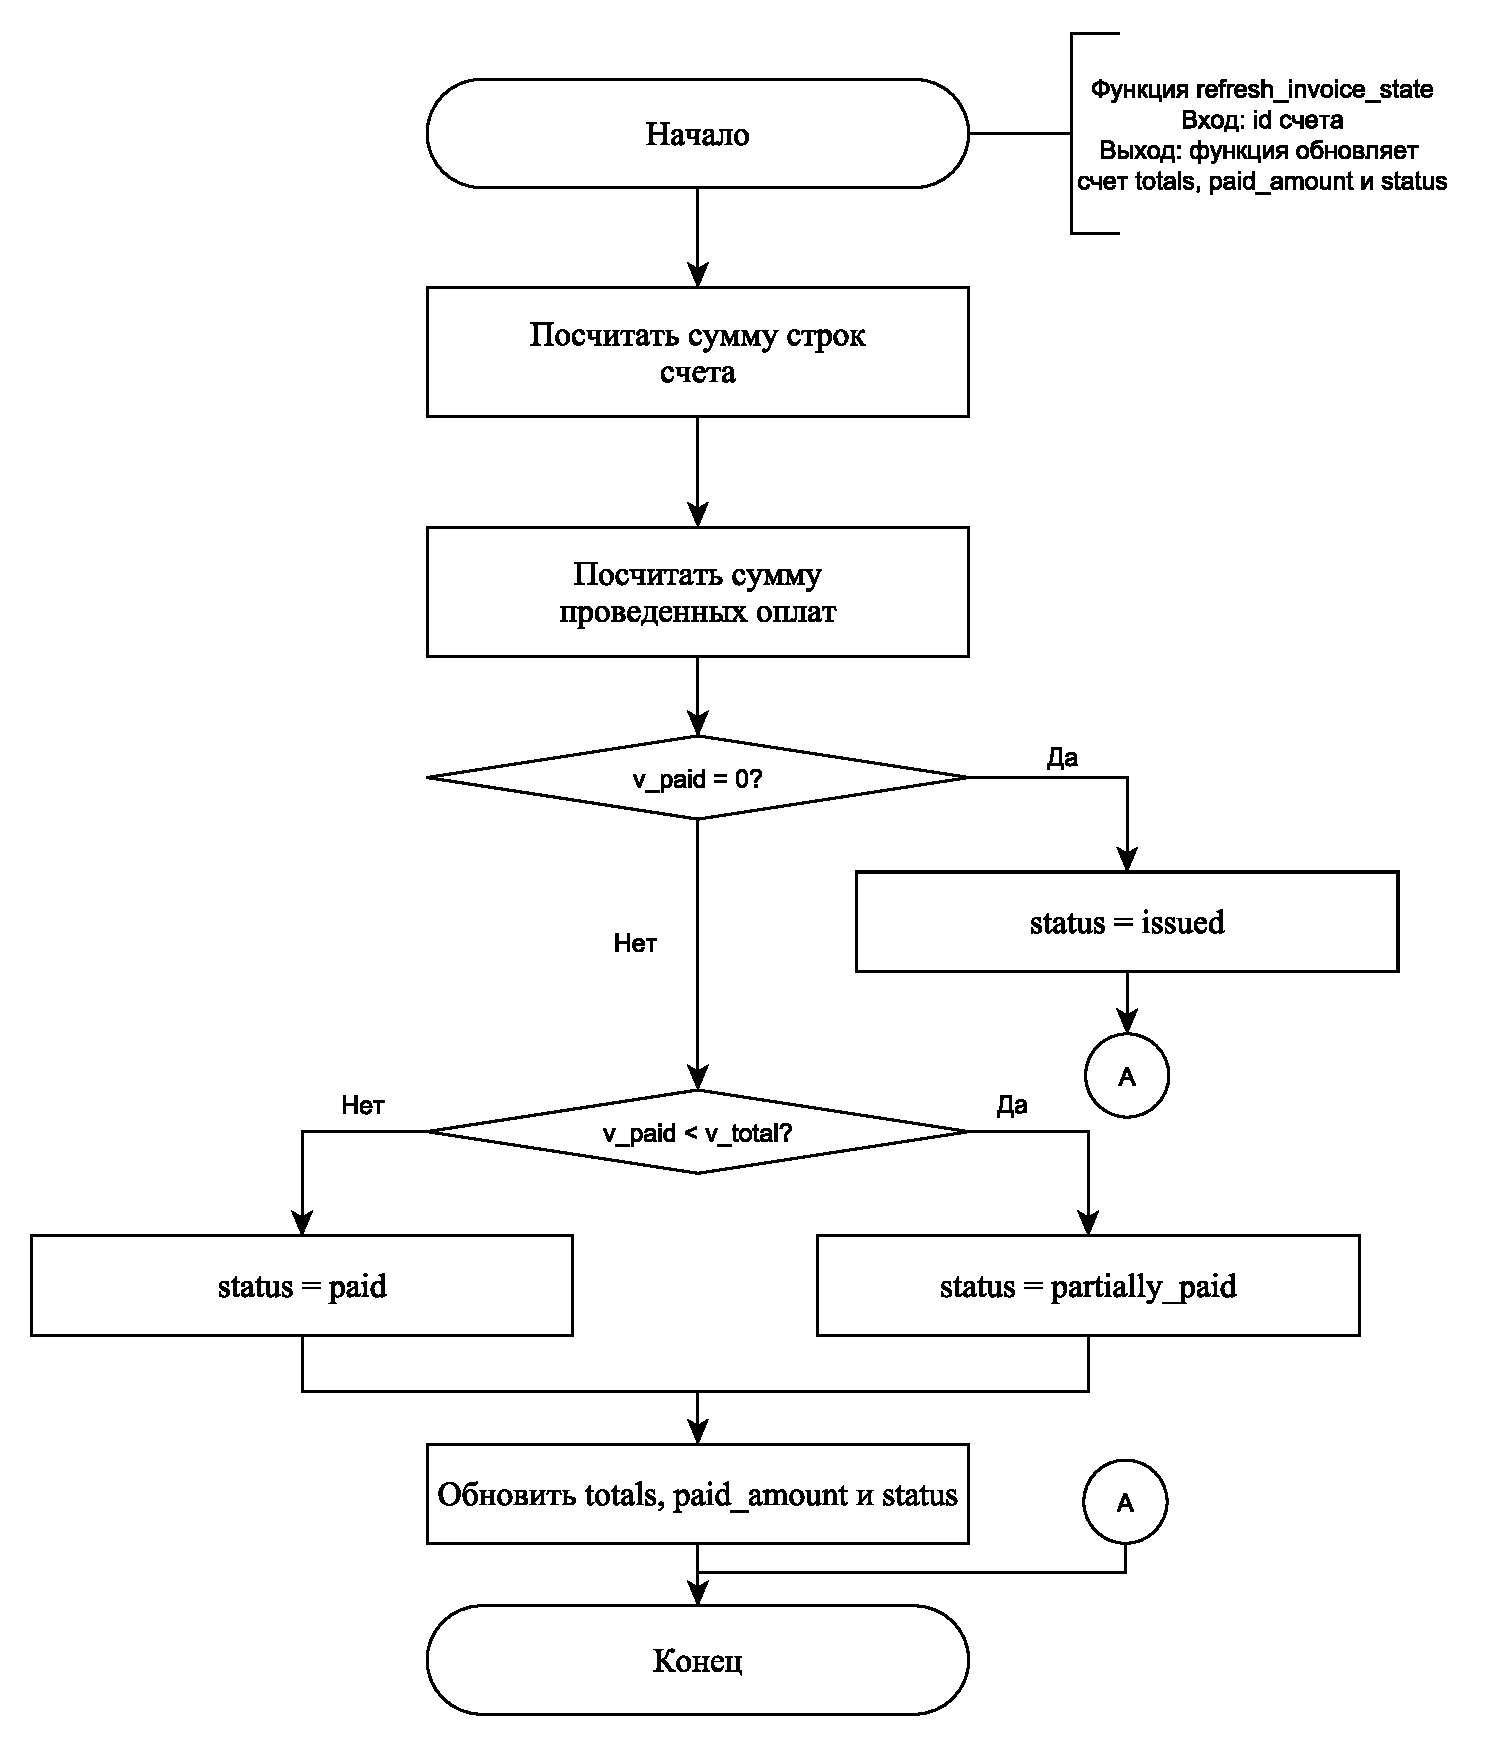
\includegraphics[width=0.74\textwidth]{figures/yed_refresh_invoice_state.pdf}
    \caption{Схема функции \texttt{refresh\_invoice\_state}}
    \label{fig:design-refresh-invoice-state}
\end{figure}

Схема триггеров пересчета счета приведена на рисунке~\ref{fig:design-refresh-invoice-triggers}.

Триггеры \texttt{trg\_\allowbreak{}invoice\_\allowbreak{}items\_\allowbreak{}refresh\_\allowbreak{}invoice} и \texttt{trg\_\allowbreak{}payments\_\allowbreak{}refresh\_\allowbreak{}invoice} срабатывают после изменения строк счета или оплат, определяют идентификатор счета и вызывают функцию \texttt{refresh\_\allowbreak{}invoice\_\allowbreak{}state}.

\begin{figure}[H]
    \centering
    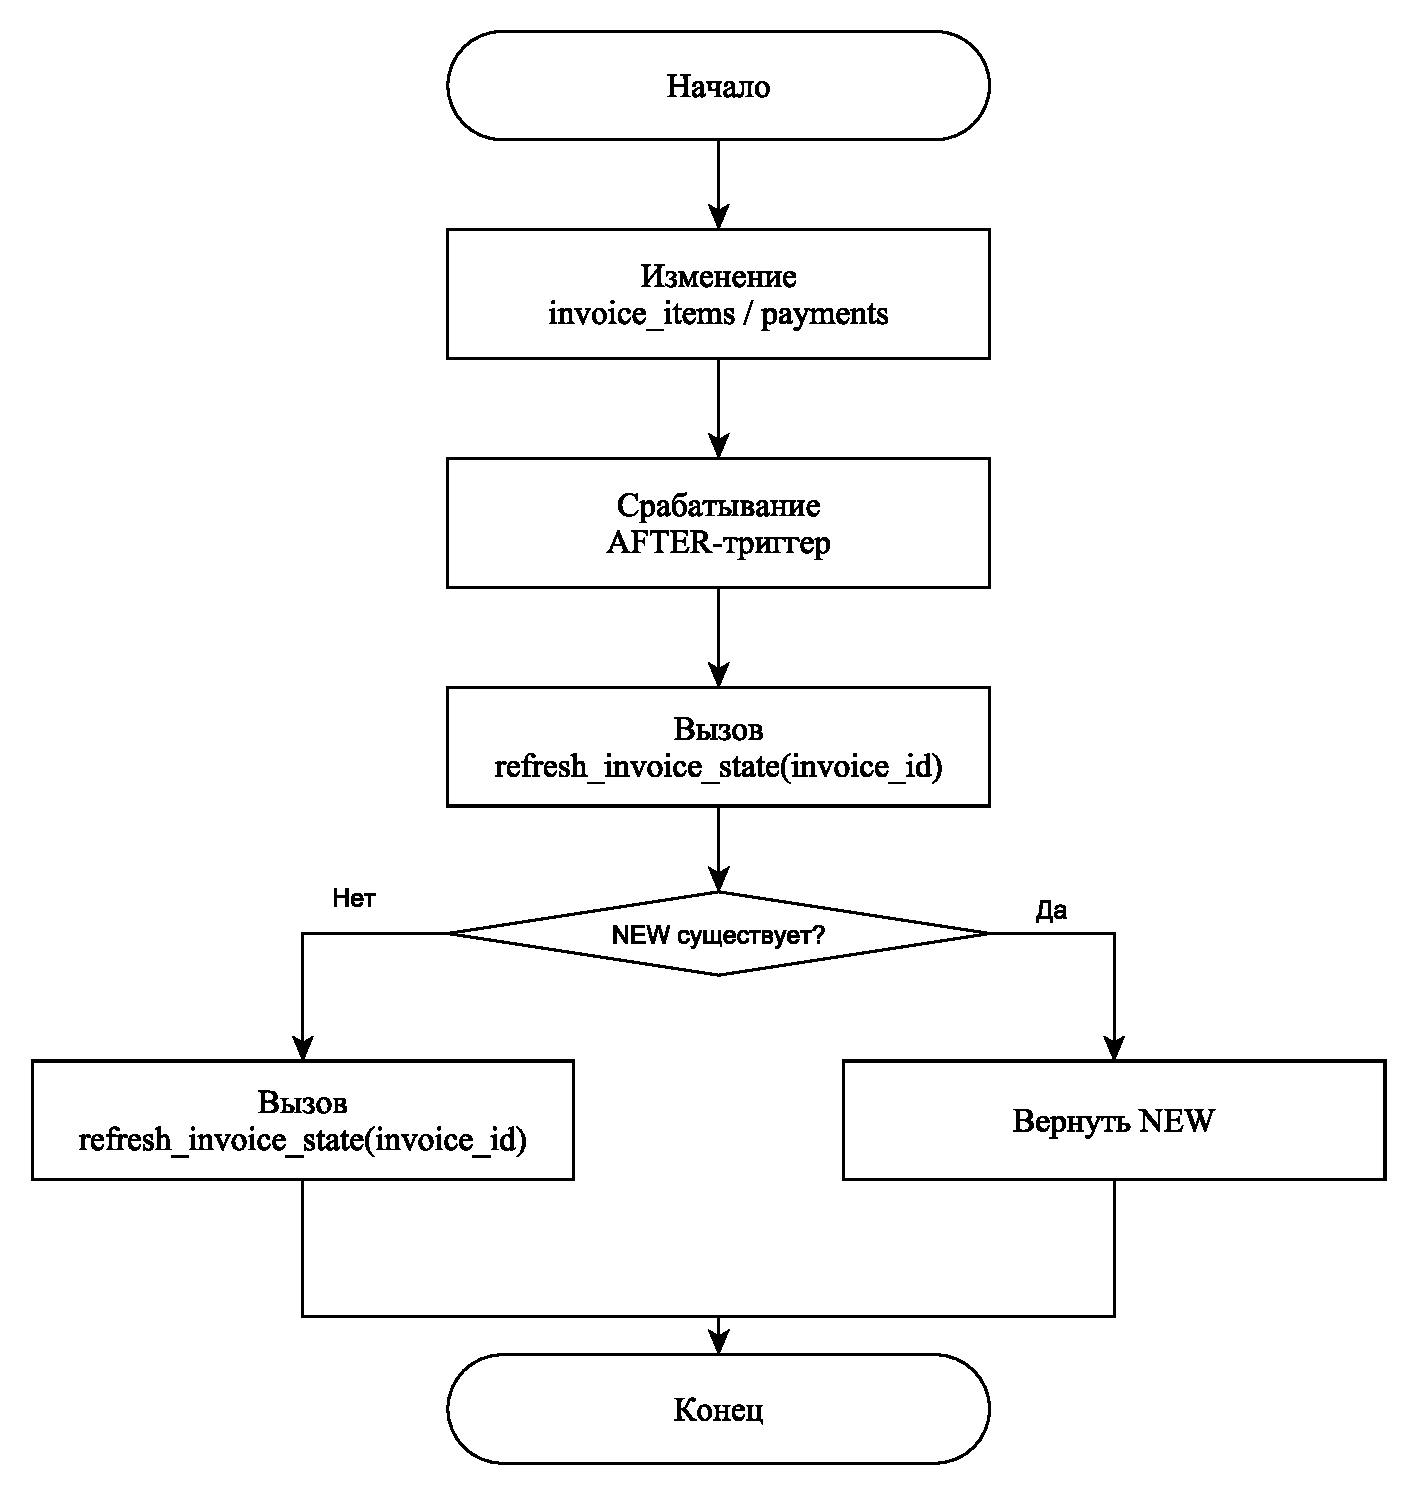
\includegraphics[width=0.68\textwidth]{figures/yed_refresh_invoice_triggers.pdf}
    \caption{Схема триггеров пересчета счета}
    \label{fig:design-refresh-invoice-triggers}
\end{figure}



Перечень триггеров базы данных приведен в таблице~\ref{tab:db-triggers}.

\begin{table}[H]
    \centering
    \caption{Триггеры базы данных}
    \label{tab:db-triggers}
    \footnotesize
    \renewcommand{\arraystretch}{1.12}
    \setlength{\tabcolsep}{4pt}
    \begin{tabularx}{\textwidth}{|>{\raggedright\arraybackslash}p{4.10cm}|>{\raggedright\arraybackslash}p{4.75cm}|>{\raggedright\arraybackslash}X|}
        \hline
        Имя триггера & Таблица и событие & Назначение \tabularnewline
        \hline
        \parbox[t]{4.10cm}{\raggedright{\scriptsize\texttt{trg\_\*\_}}\newline {\scriptsize\texttt{updated\_at}}} &
        \parbox[t]{4.75cm}{\raggedright{\scriptsize\texttt{users, patients,}}\newline {\scriptsize\texttt{doctors, services,}}\newline {\scriptsize\texttt{appointments, visits,}}\newline {\scriptsize\texttt{invoices,}}\newline {\scriptsize\texttt{doctor\_availability,}}\newline {\scriptsize\texttt{doctor\_absences;}}\newline событие {\scriptsize\texttt{BEFORE UPDATE}}} &
        Автоматическое обновление поля \texttt{updated\_at} \tabularnewline
        \hline
        \parbox[t]{4.10cm}{\raggedright{\scriptsize\texttt{trg\_invoice\_items\_}}\newline {\scriptsize\texttt{refresh\_invoice}}} &
        \parbox[t]{4.75cm}{\raggedright{\scriptsize\texttt{billing.invoice\_items;}}\newline событие {\scriptsize\texttt{AFTER INSERT,}}\newline {\scriptsize\texttt{UPDATE, DELETE}}} &
        Пересчет суммы и статуса счета \tabularnewline
        \hline
        \parbox[t]{4.10cm}{\raggedright{\scriptsize\texttt{trg\_payments\_}}\newline {\scriptsize\texttt{refresh\_invoice}}} &
        \parbox[t]{4.75cm}{\raggedright{\scriptsize\texttt{billing.payments;}}\newline событие {\scriptsize\texttt{AFTER INSERT,}}\newline {\scriptsize\texttt{UPDATE, DELETE}}} &
        Пересчет суммы оплат и статуса счета \tabularnewline
        \hline
    \end{tabularx}
\end{table}

\section{Ролевая модель базы данных}

Следует различать прикладные роли системы и роли базы данных.

Прикладные роли описывают, кто работает в интерфейсе системы, например пациент, администратор или врач. Ролевая модель базы данных описывает роли PostgreSQL и выданные им привилегии на объекты схемы.

В конструкторском разделе требуется именно ролевая модель на уровне базы данных.

В реализованной схеме используются три роли PostgreSQL:
\begin{itemize}
    \item \texttt{clinic\_owner};
    \item \texttt{clinic\_api};
    \item \texttt{clinic\_reporting}.
\end{itemize}
Их назначение приведено в таблице~\ref{tab:db-role-model}.

\begin{table}[H]
    \centering
    \caption{Ролевая модель базы данных}
    \label{tab:db-role-model}
    \footnotesize
    \renewcommand{\arraystretch}{1.1}
    \setlength{\tabcolsep}{4pt}
    \begin{tabularx}{\textwidth}{|>{\raggedright\arraybackslash}p{3.0cm}|>{\raggedright\arraybackslash}p{3.3cm}|>{\raggedright\arraybackslash}X|}
        \hline
        Роль PostgreSQL & Назначение & Предоставляемые права \tabularnewline
        \hline
        \texttt{clinic\_owner} & \begin{tabular}[t]{@{}l@{}}Владелец схемы\tabularnewline базы данных\end{tabular} & \begin{tabular}[t]{@{}l@{}}Создание и изменение схем, таблиц,\tabularnewline индексов, процедур, триггеров и ролей\end{tabular} \tabularnewline
        \hline
        \texttt{clinic\_api} & \begin{tabular}[t]{@{}l@{}}Роль backend-\tabularnewline приложения\end{tabular} & \begin{tabular}[t]{@{}l@{}}USAGE на схемы;\tabularnewline SELECT, INSERT, UPDATE, DELETE\tabularnewline для рабочих таблиц;\tabularnewline EXECUTE для процедур и функций\end{tabular} \tabularnewline
        \hline
        \begin{tabular}[t]{@{}l@{}}\texttt{clinic\_}\tabularnewline\texttt{reporting}\end{tabular} & \begin{tabular}[t]{@{}l@{}}Роль отчетов\tabularnewline и аналитики\end{tabular} & \begin{tabular}[t]{@{}l@{}}Доступ только на чтение к данным,\tabularnewline необходимым для формирования отчетов\end{tabular} \tabularnewline
        \hline
    \end{tabularx}
\end{table}
\normalsize

Прикладные роли пользователей не дублируются отдельными SQL-ролями. Они контролируются на уровне приложения и работают через backend, использующий роль \texttt{clinic\_api}.

Таким образом, разграничение доступа на уровне интерфейса и на уровне СУБД остаются разделенными и не смешиваются в одной модели.

\section{Транзакционная стратегия и требования к кэшированию}

Критические операции --- запись на прием, отмена записи, проведение приема и регистрация оплаты --- выполняются в транзакционном контексте.

Контроль согласованности сосредоточен в PostgreSQL. Он обеспечивается сочетанием транзакций, ограничений целостности, диапазонных типов и исключающих ограничений.

Для ускорения чтения в Redis кэшируются два объекта:
\begin{itemize}
    \item текущий прайс-лист услуг по ключу \texttt{clinic:catalog:pricelist} с временем жизни 600 секунд;
    \item расписание врача по ключу вида \texttt{clinic:schedule:doctor:...} с временем жизни 600 секунд.
\end{itemize}

Кэш расписания инвалидируется после записи на прием, отмены записи и проведения приема. Кэш прайс-листа обновляется при повторном чтении после истечения времени жизни записи.

\section{Вывод}

В конструкторском разделе спроектирована структура базы данных медицинской клиники, доказано соответствие 3НФ, описаны ограничения целостности, процедуры, функции, триггеры, ролевая модель базы данных и правила кэширования. Полученная схема соответствует требованиям проекта и обеспечивает основу для дальнейшей реализации приложения.

\clearpage

% Технологический раздел
\chapter{Технологический раздел}

В данном разделе описаны выбранные средства реализации базы данных и приложения, состав реализованной базы данных, ограничения целостности, роли базы данных, интерфейс доступа к данным и порядок тестирования функций базы данных.

\section{Средства реализации}

Для реализации базы данных выбрана СУБД PostgreSQL. Данная СУБД поддерживает ACID-транзакции, домены, перечислимые типы, индексы, триггеры, хранимые функции и процедуры, диапазонные типы данных, а также ограничение EXCLUDE. Эти возможности позволяют перенести критические правила предметной области на уровень базы данных: запрет пересечения записей по времени, проверку актуальности цены, пересчет состояния счета и контроль допустимых статусов.

PostgreSQL также подходит для выбранной предметной области за счет развитой поддержки внешних ключей, транзакционной согласованности и диапазонных типов данных~\cite{postgres_range}. Расширение btree\_gist используется для ограничения пересечения временных интервалов. Для генерации UUID применяется расширение pgcrypto.

Для серверной части выбраны язык Go~\cite{go_docs}, пакет database/sql, драйвер pgx и фреймворк Gin~\cite{gin_docs}. Такое сочетание позволяет реализовать REST API и разделить код backend-приложения на слои Handler, Service и Repository. При этом критическая бизнес-логика не дублируется в приложении, а вызывается через функции PostgreSQL.

В качестве программного интерфейса доступа к данным выбран стандартный интерфейс Go database/sql с драйвером pgx. Выбор обусловлен тем, что данный интерфейс соответствует стеку backend-приложения, поддерживает параметризованные SQL-запросы, транзакции, работу через пул соединений и прямой вызов функций PostgreSQL. Универсальные интерфейсы ODBC, ADO.NET и JDBC в данном проекте не выбраны, так как они ориентированы на другие технологические платформы или требуют лишнего промежуточного слоя. Полноценная ORM также не использована, поскольку в курсовой работе требуется явно показать работу с реализованными функциями, триггерами и ограничениями базы данных.

Для клиентской части выбраны React~\cite{react_docs} и TypeScript~\cite{typescript_docs}. Клиентское приложение используется как демонстрационный интерфейс для регистрации пациента, просмотра прайс-листа, просмотра расписания, записи на прием, отмены записи, проведения приема и регистрации оплаты.

Для кэширования часто запрашиваемых данных используется Redis~\cite{redis_docs}. В кэш помещаются актуальный прайс-лист услуг и представление расписания врача за выбранный интервал. Сводная информация о выбранных средствах приведена в таблице~\ref{tab:stack}.

\begin{table}[H]
    \centering
    \caption{Выбранные средства реализации}
    \label{tab:stack}
    \small
    \begin{tabularx}{\textwidth}{|>{\raggedright\arraybackslash}p{3.3cm}|>{\raggedright\arraybackslash}p{4.2cm}|>{\raggedright\arraybackslash}X|}
        \hline
        Слой & Технология & Назначение \tabularnewline
        \hline
        Frontend & React + TypeScript & Реализация пользовательского интерфейса \tabularnewline
        \hline
        Backend & Go + Gin & Реализация REST API и серверной логики \tabularnewline
        \hline
        Доступ к БД & database/sql + pgx & Выполнение SQL-запросов и вызов функций PostgreSQL \tabularnewline
        \hline
        СУБД & PostgreSQL & Хранение данных, контроль целостности, индексы, функции и триггеры \tabularnewline
        \hline
        InMemory СУБД & Redis & Кэширование прайс-листа и расписания врачей \tabularnewline
        \hline
        API & REST & Обмен данными между frontend и backend \tabularnewline
        \hline
    \end{tabularx}
\end{table}
\normalsize

\section{Состав реализованной базы данных}

База данных реализована в сценарии db/schema.sql. В ней созданы логические схемы security, catalog, medical, scheduling и billing. Такое разбиение отделяет учетные записи и роли от справочников, медицинских данных, расписания и финансового контура.

Состав реализованных таблиц приведен в таблице~\ref{tab:implemented-entities}.

\begin{table}[H]
    \centering
    \caption{Сущности реализованной базы данных}
    \label{tab:implemented-entities}
    \footnotesize
    \renewcommand{\arraystretch}{1.08}
    \begin{tabularx}{\textwidth}{|>{\raggedright\arraybackslash}p{3.5cm}|>{\raggedright\arraybackslash}X|}
        \hline
        Схема & Реализованные сущности \tabularnewline
        \hline
        security & roles, users, user\_roles. Сущности отвечают за учетные записи, прикладные роли и связь многие-ко-многим между пользователями и ролями. \tabularnewline
        \hline
        catalog & specialties, services, service\_prices, представление current\_price\_list. Сущности описывают специальности, услуги и историю цен. \tabularnewline
        \hline
        medical & patients, doctors, doctor\_services, visits, visit\_services. Сущности хранят данные пациентов, врачей, оказанных услуг и результатов приема. \tabularnewline
        \hline
        scheduling & doctor\_availability, doctor\_absences, appointments. Сущности реализуют расписание, периоды отсутствия врача и записи пациентов на прием. \tabularnewline
        \hline
        billing & invoices, invoice\_items, payments. Сущности отвечают за формирование счетов, строки счетов и регистрацию оплат. \tabularnewline
        \hline
    \end{tabularx}
\end{table}
\normalsize

Связи многие-ко-многим реализованы через отдельные промежуточные таблицы. В качестве первичных ключей основных сущностей используются UUID. Фрагмент реализации сущности записи на прием приведен в листинге~\ref{lst:appendix-appointments} приложения~А.

\section{Реализованные ограничения целостности}

В базе данных реализованы домены, перечислимые типы, первичные и внешние ключи, ограничения уникальности, проверки значений, диапазонные ограничения и индексы. Основные группы ограничений приведены в таблице~\ref{tab:implemented-constraints}.

\begin{table}[H]
    \centering
    \caption{Реализованные ограничения целостности}
    \label{tab:implemented-constraints}
    \footnotesize
    \renewcommand{\arraystretch}{1.1}
    \begin{tabularx}{\textwidth}{|>{\raggedright\arraybackslash}p{4.0cm}|>{\raggedright\arraybackslash}X|}
        \hline
        Группа ограничений & Реализация \tabularnewline
        \hline
        Форматы контактных данных & Домены security.email\_address и security.phone\_number проверяют формат e-mail и телефона. \tabularnewline
        \hline
        Состояния сущностей & Перечислимые типы user\_status, patient\_status, doctor\_status, service\_status, appointment\_status, invoice\_status, payment\_status. \tabularnewline
        \hline
        Ссылочная целостность & Внешние ключи связывают пользователей с ролями, врачей со специальностями, записи с пациентами и врачами, визиты с записями, счета с визитами, оплаты со счетами. \tabularnewline
        \hline
        Уникальность & Уникальны логины пользователей, коды ролей, коды услуг, названия специальностей, связь врача с учетной записью, связь визита с записью и связь счета с визитом. \tabularnewline
        \hline
        Числовые проверки & Ограничения CHECK запрещают отрицательные суммы, нулевое количество услуг, некорректную длительность приема и дату рождения позже текущей даты. \tabularnewline
        \hline
        Временные интервалы & Для цен, доступности, отсутствий и записей используются диапазоны TSTZRANGE; дополнительно проверяется, что окончание интервала позже начала. \tabularnewline
        \hline
        Запрет пересечений & Ограничения EXCLUDE запрещают пересечение периодов цен одной услуги, активных интервалов доступности врача и активных записей одного врача. \tabularnewline
        \hline
    \end{tabularx}
\end{table}
\normalsize

Для ускорения ключевых операций созданы индексы по статусам пользователей, пациентов, врачей и услуг, по телефону пациента, по специальности врача, по истории цен, по расписанию врача, по истории пациента, по счетам пациента и по оплатам счета. Фрагменты реализации ограничений целостности приведены в листинге~\ref{lst:appendix-constraints} приложения~А.

\section{Реализованные функции и триггеры}

На стороне базы данных реализованы функции, инкапсулирующие основные правила предметной области. Перечень функций и триггеров приведен в таблице~\ref{tab:implemented-db-functions}. Схемы алгоритмов данных функций и триггеров приведены в конструкторском разделе на рисунках~\ref{fig:yed-set-updated-at}--\ref{fig:design-refresh-invoice-triggers}.

\begin{table}[H]
    \centering
    \caption{Реализованные функции и триггеры базы данных}
    \label{tab:implemented-db-functions}
    \footnotesize
    \renewcommand{\arraystretch}{1.08}
    \begin{tabularx}{\textwidth}{|>{\raggedright\arraybackslash}p{4.4cm}|>{\raggedright\arraybackslash}X|}
        \hline
        Объект & Назначение \tabularnewline
        \hline
        \begin{tabular}[t]{@{}l@{}}security.\tabularnewline set\_updated\_at\end{tabular} & Обновляет поле updated\_at перед изменением записи. \tabularnewline
        \hline
        \begin{tabular}[t]{@{}l@{}}security.\tabularnewline has\_role\end{tabular} & Проверяет наличие прикладной роли у пользователя. \tabularnewline
        \hline
        \begin{tabular}[t]{@{}l@{}}catalog.\tabularnewline get\_service\_price\end{tabular} & Возвращает актуальную цену услуги на заданный момент времени. \tabularnewline
        \hline
        \begin{tabular}[t]{@{}l@{}}scheduling.\tabularnewline book\_appointment\end{tabular} & Создает запись на прием после проверки пациента, врача, услуги, доступности врача и отсутствия врача. \tabularnewline
        \hline
        \begin{tabular}[t]{@{}l@{}}scheduling.\tabularnewline cancel\_appointment\end{tabular} & Отменяет запись с учетом статуса записи и роли пользователя, инициировавшего отмену. \tabularnewline
        \hline
        \begin{tabular}[t]{@{}l@{}}medical.\tabularnewline complete\_visit\end{tabular} & Создает визит, фиксирует оказанные услуги, формирует счет и переводит запись в состояние completed. \tabularnewline
        \hline
        \begin{tabular}[t]{@{}l@{}}billing.\tabularnewline register\_payment\end{tabular} & Регистрирует оплату и инициирует пересчет состояния счета. \tabularnewline
        \hline
        \begin{tabular}[t]{@{}l@{}}billing.\tabularnewline refresh\_invoice\_state\end{tabular} & Пересчитывает итоговую сумму счета, сумму оплат и статус счета. \tabularnewline
        \hline
        trg\_\*\_updated\_at & Триггеры автоматического обновления поля updated\_at. \tabularnewline
        \hline
        \begin{tabular}[t]{@{}l@{}}trg\_invoice\_items\_\tabularnewline refresh\_invoice,\tabularnewline trg\_payments\_\tabularnewline refresh\_invoice\end{tabular} & Триггеры пересчета счета после изменения строк счета или оплат. \tabularnewline
        \hline
    \end{tabularx}
\end{table}
\normalsize

Реализация перечисленных объектов находится в сценарии db/schema.sql. Функции созданы операторами CREATE OR REPLACE FUNCTION, а автоматический вызов служебной логики обеспечивается триггерами CREATE TRIGGER. Функция получения актуальной цены услуги приведена в листинге~\ref{lst:appendix-get-service-price} приложения~А, фрагмент функции записи на прием -- в листинге~\ref{lst:appendix-book-appointment}, а триггеры пересчета состояния счета -- в листинге~\ref{lst:appendix-refresh-invoice-triggers}.

\section{Ролевая модель базы данных}

На уровне PostgreSQL реализованы три роли базы данных. Они отделяют владение схемой, работу backend-приложения и доступ к отчетным данным.

\begin{table}[H]
    \centering
    \caption{Ролевая модель на уровне базы данных}
    \label{tab:technology-db-roles}
    \footnotesize
    \renewcommand{\arraystretch}{1.08}
    \begin{tabularx}{\textwidth}{|>{\raggedright\arraybackslash}p{3.2cm}|>{\raggedright\arraybackslash}p{3.8cm}|>{\raggedright\arraybackslash}X|}
        \hline
        Роль & Назначение & Права \tabularnewline
        \hline
        clinic\_owner & Владелец структуры базы данных & Создание и изменение схем, таблиц, индексов, функций, триггеров и ролей. \tabularnewline
        \hline
        clinic\_api & Роль backend-приложения & USAGE на схемы, SELECT, INSERT, UPDATE, DELETE на таблицы, EXECUTE на функции. \tabularnewline
        \hline
        \begin{tabular}[t]{@{}l@{}}clinic\_\tabularnewline reporting\end{tabular} & Роль отчетов и аналитики & SELECT на таблицы и USAGE на схемы без прав изменения данных. \tabularnewline
        \hline
    \end{tabularx}
\end{table}
\normalsize

Прикладные роли пациента, администратора и врача хранятся в таблицах security.roles и security.user\_roles. Они используются backend-приложением и функцией has\_role для проверки бизнес-правил, например права администратора отменять запись без ограничения в 24 часа. Фрагмент SQL-сценария создания ролей и выдачи прав приведен в листинге~\ref{lst:appendix-db-roles} приложения~А.

\section{Разработка интерфейса доступа к базе данных}

Frontend не обращается к базе данных напрямую. Все операции выполняются через REST API backend-приложения. Backend-слой валидирует входные данные, вызывает репозитории и функции PostgreSQL, а затем возвращает результат клиенту в формате JSON.

Реализация доступа к данным построена по трехслойной схеме: Handler, Service и Repository. Обработчики HTTP-запросов отвечают за прием и валидацию DTO, сервисный слой выполняет прикладную координацию и работу с Redis-кэшем, а репозитории являются единственным слоем, напрямую выполняющим SQL-запросы через database/sql. Такой интерфейс отделяет клиентское приложение от конкретной СУБД и одновременно сохраняет явный доступ к функциям PostgreSQL, разработанным в рамках курсовой работы.

Компонентная структура приложения показана на рисунке~\ref{fig:technology-app-components}. Пользователь работает с React-интерфейсом, frontend отправляет REST-запросы в backend, а backend последовательно передает обработку на уровни Handler, Service и Repository. Репозиторий обращается к PostgreSQL как к основной СУБД и к Redis как к InMemory-хранилищу кэшируемых представлений.

\begin{figure}[H]
    \centering
    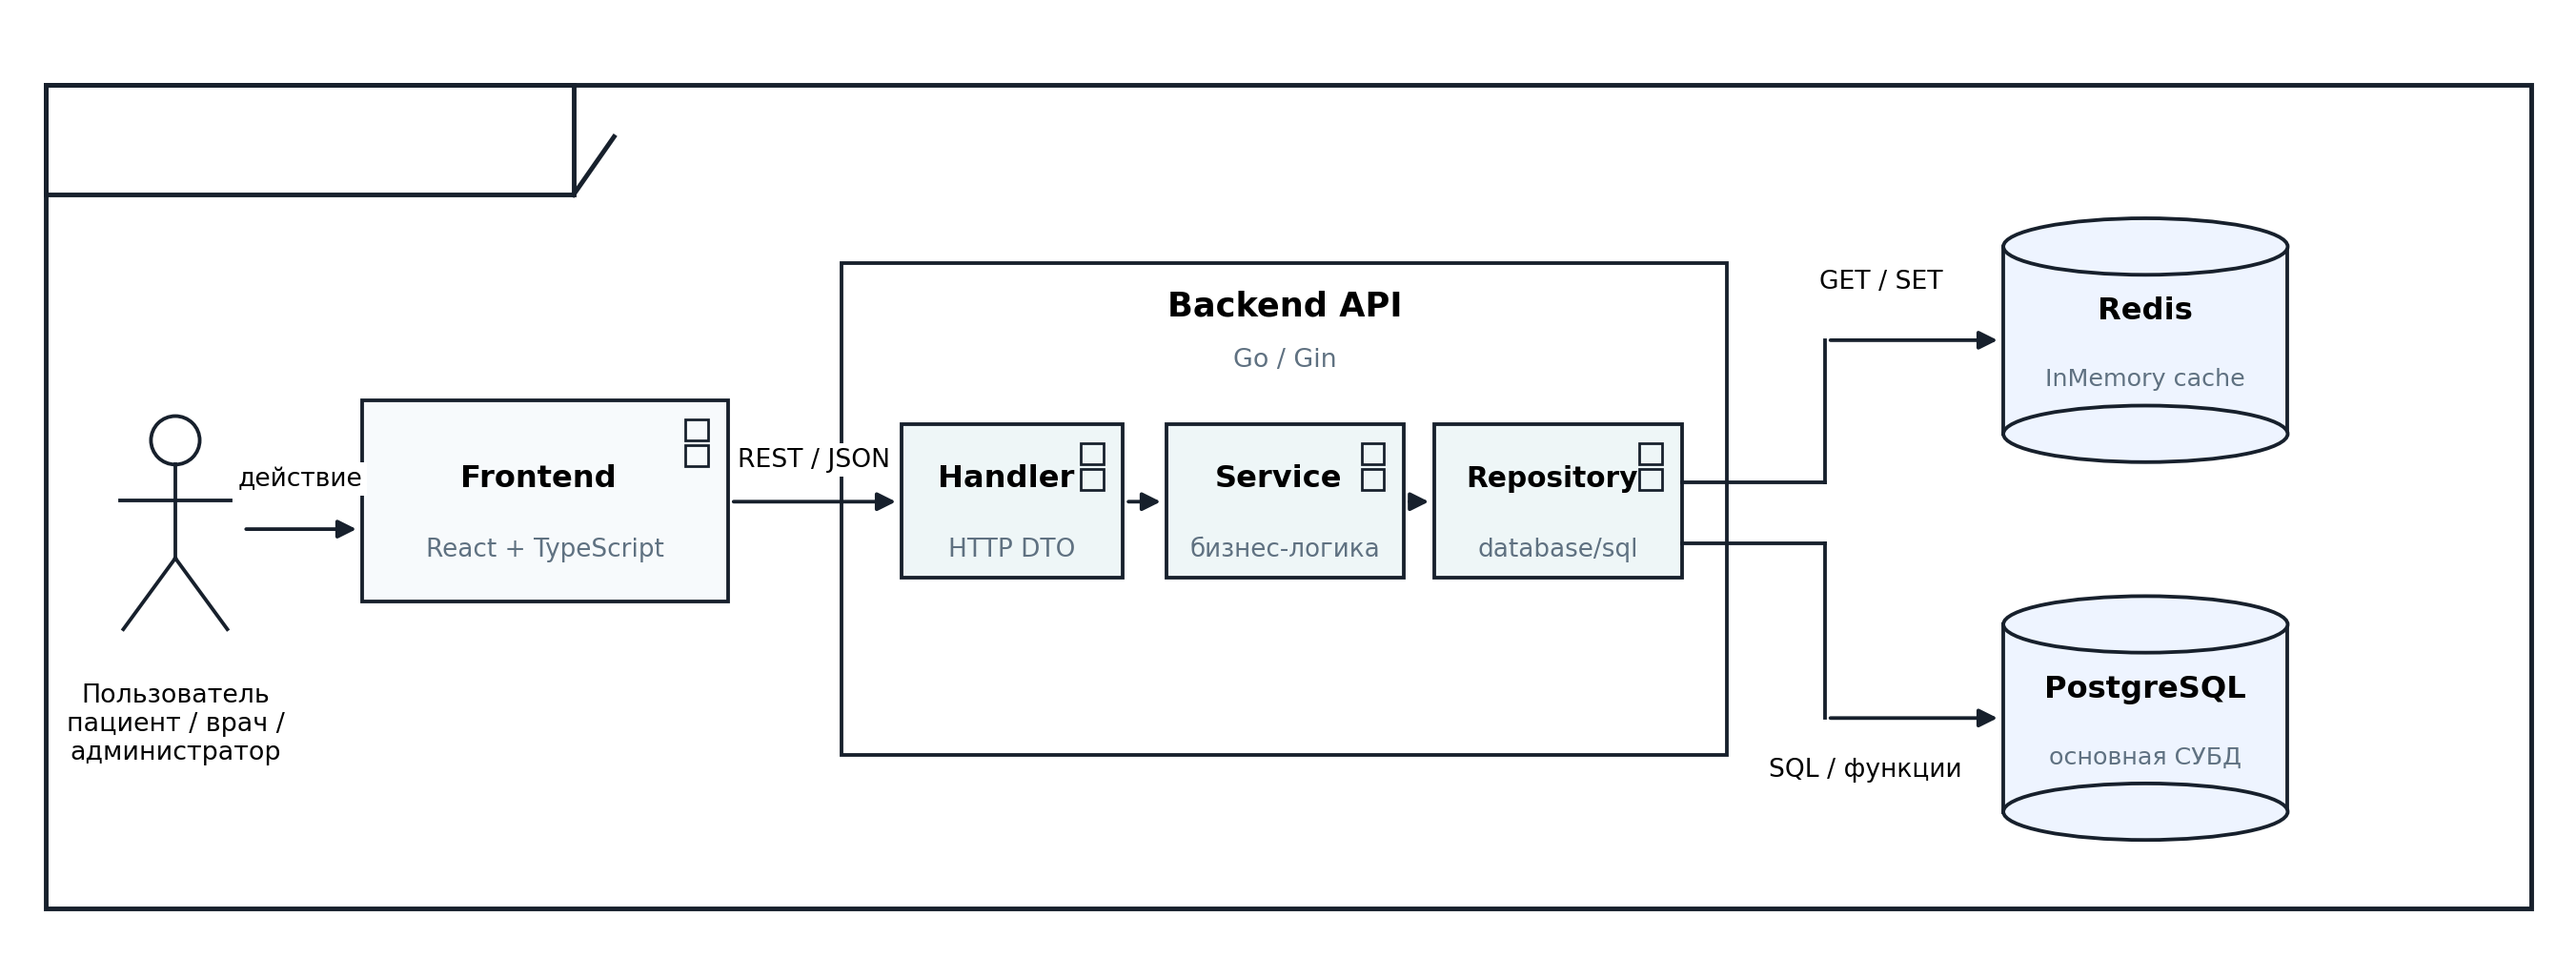
\includegraphics[width=\textwidth]{figures/technology_app_components.png}
    \caption{UML-диаграмма компонентов приложения}
    \label{fig:technology-app-components}
\end{figure}

Последовательность взаимодействия приложения с Redis и PostgreSQL при работе с кэшем показана на рисунке~\ref{fig:technology-cache-sequence}. На схеме отдельно приведены чтение данных через Redis-кэш и изменение данных с последующей инвалидацией кэша расписания. При отсутствии значения в Redis backend читает данные из PostgreSQL и сохраняет JSON-представление в кэш; при наличии значения результат возвращается без обращения к основной СУБД.

\begin{figure}[H]
    \centering
    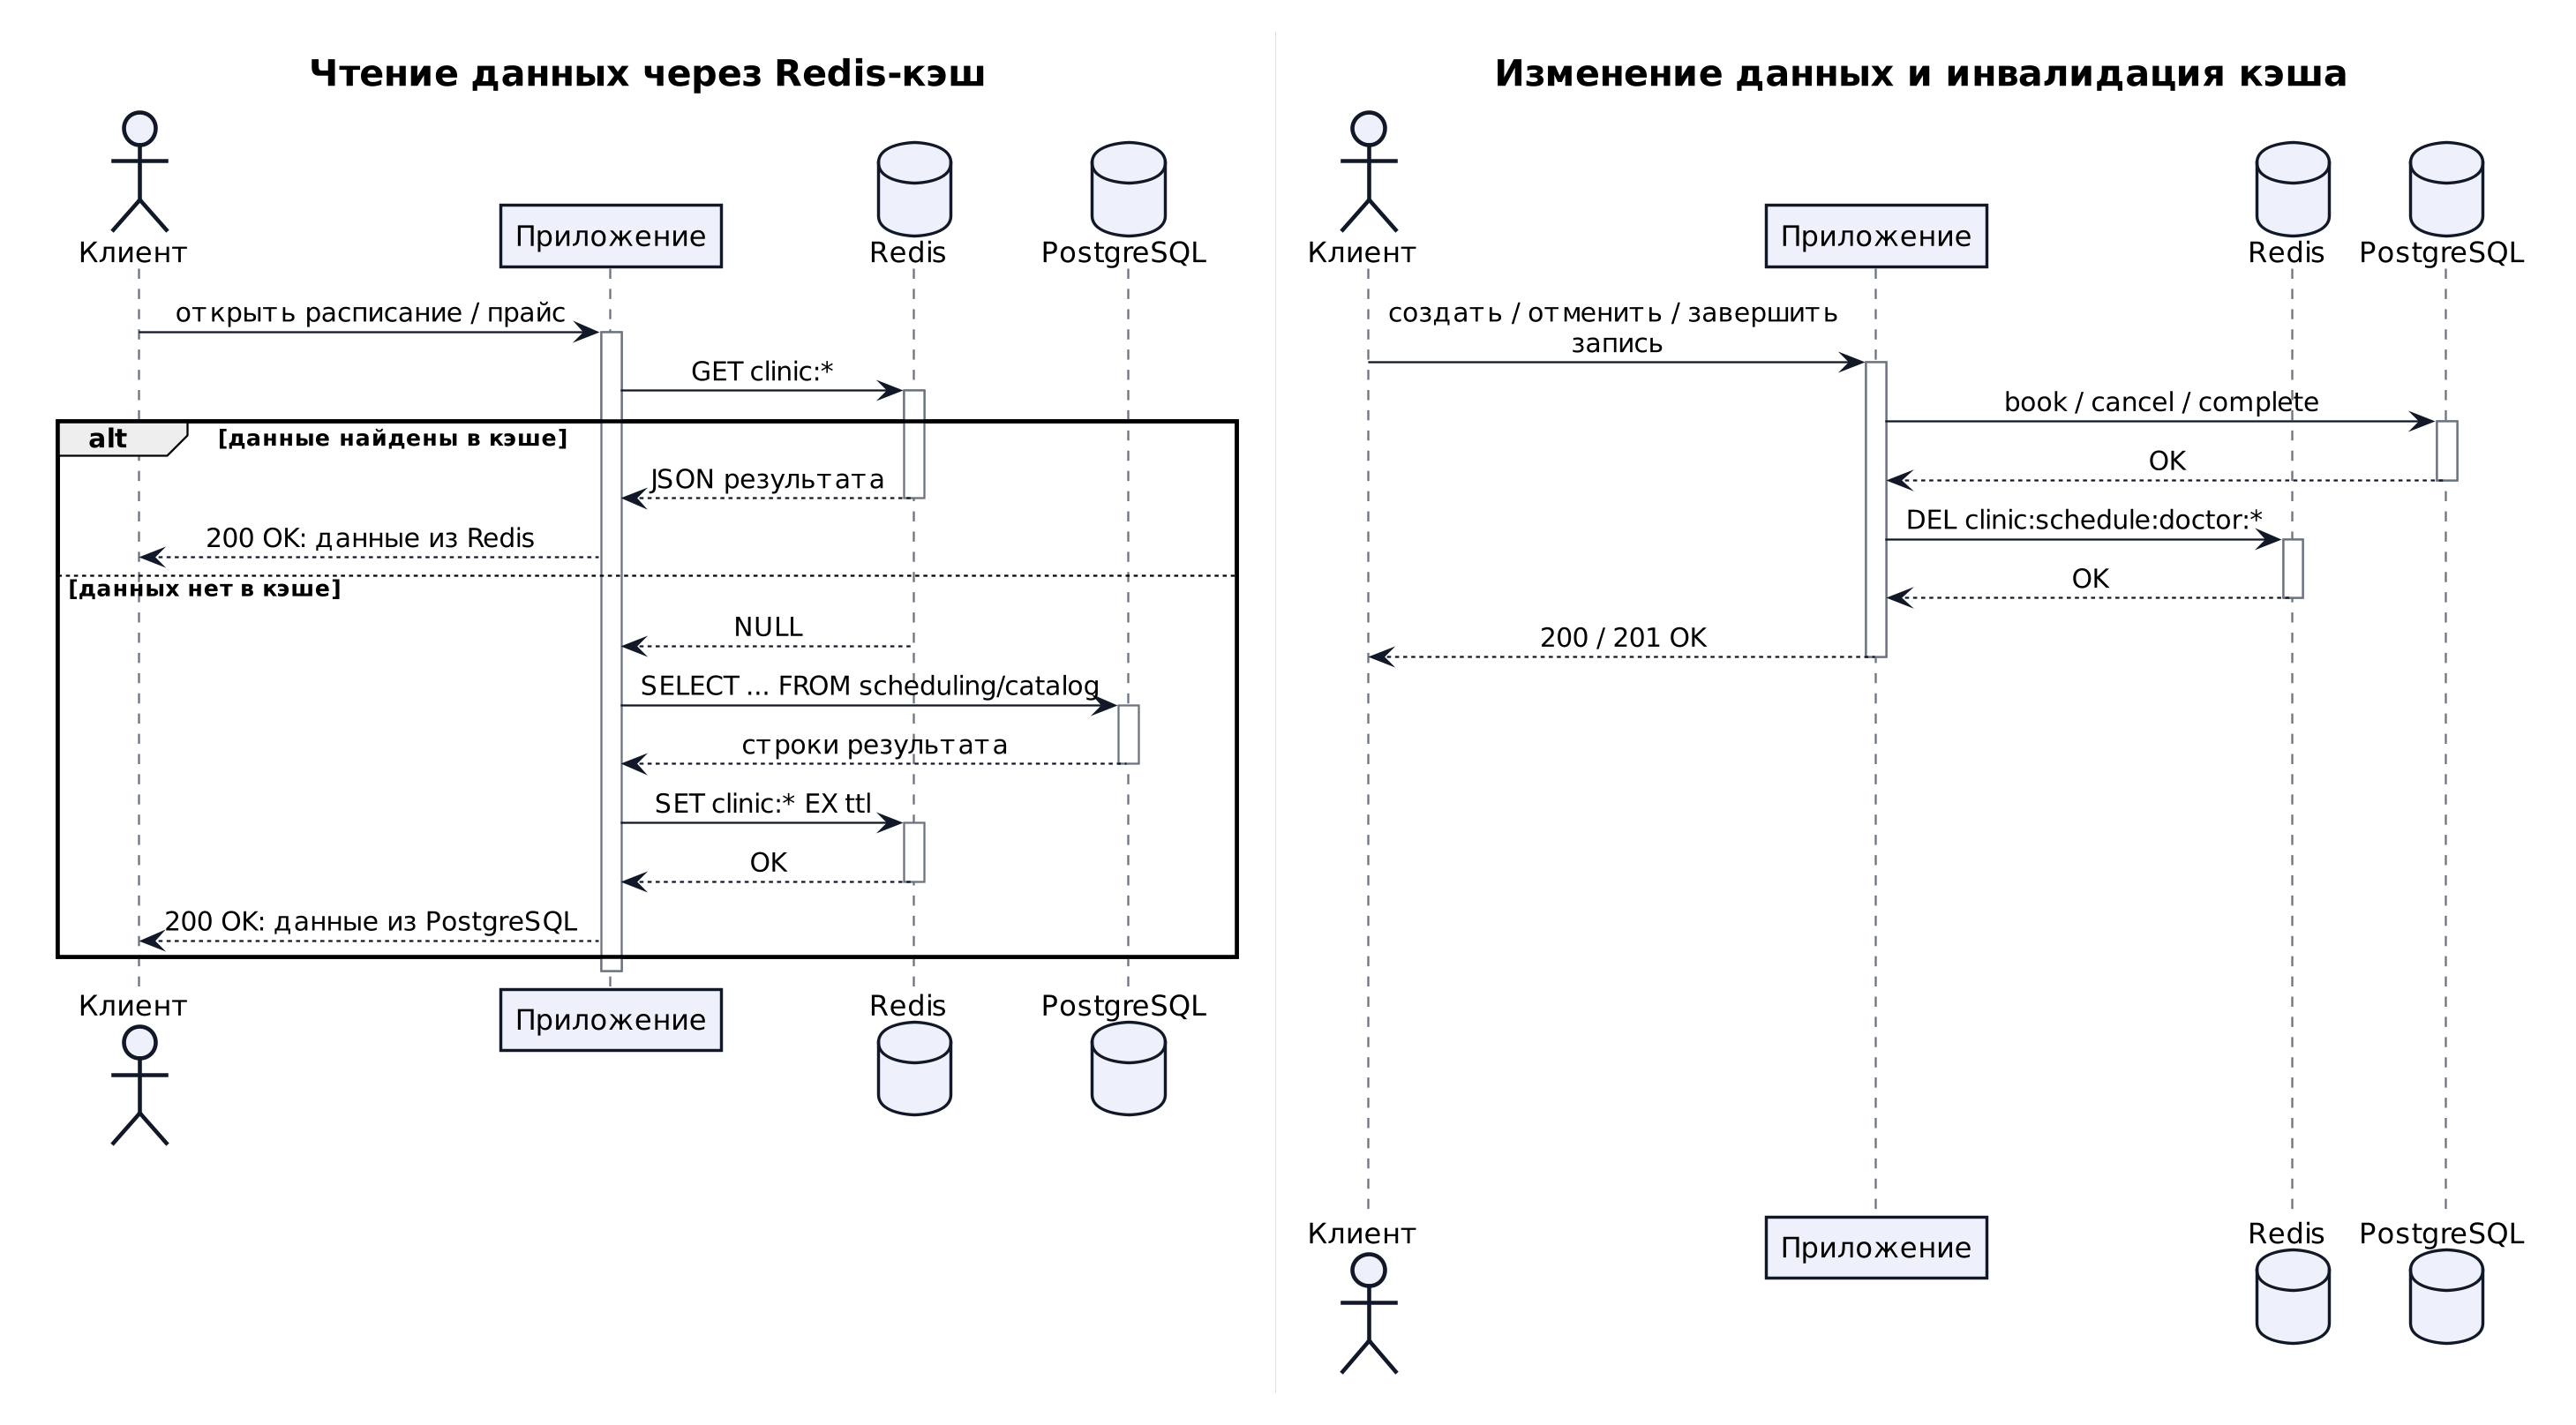
\includegraphics[width=\textwidth,height=0.82\textheight,keepaspectratio]{figures/technology_cache_sequence_plantuml_pair.png}
    \caption{UML-диаграмма последовательности доступа к PostgreSQL и Redis}
    \label{fig:technology-cache-sequence}
\end{figure}

\begin{table}[H]
    \centering
    \caption{Интерфейс доступа к базе данных}
    \label{tab:api-db-interface}
    \footnotesize
    \renewcommand{\arraystretch}{1.08}
    \begin{tabularx}{\textwidth}{|>{\raggedright\arraybackslash}p{4.4cm}|>{\raggedright\arraybackslash}p{4.2cm}|>{\raggedright\arraybackslash}X|}
        \hline
        Маршрут REST API & Обращение к базе данных & Назначение \tabularnewline
        \hline
        \begin{tabular}[t]{@{}l@{}}POST\tabularnewline /api/v1/patients\end{tabular} & medical.patients & Регистрация пациента. \tabularnewline
        \hline
        \begin{tabular}[t]{@{}l@{}}GET\tabularnewline /api/v1/services/\tabularnewline pricelist\end{tabular} & \begin{tabular}[t]{@{}l@{}}catalog.\tabularnewline current\_price\_list\end{tabular} & Получение актуального прайс-листа с использованием Redis-кэша. \tabularnewline
        \hline
        \begin{tabular}[t]{@{}l@{}}GET\tabularnewline /api/v1/doctors/\tabularnewline :doctorId/schedule\end{tabular} & \begin{tabular}[t]{@{}l@{}}doctor\_availability,\tabularnewline appointments\end{tabular} & Получение расписания врача с использованием Redis-кэша. \tabularnewline
        \hline
        \begin{tabular}[t]{@{}l@{}}POST\tabularnewline /api/v1/appointments\end{tabular} & \begin{tabular}[t]{@{}l@{}}scheduling.\tabularnewline book\_appointment\end{tabular} & Запись пациента на прием. \tabularnewline
        \hline
        \begin{tabular}[t]{@{}l@{}}POST\tabularnewline /api/v1/appointments/\tabularnewline :id/cancel\end{tabular} & \begin{tabular}[t]{@{}l@{}}scheduling.\tabularnewline cancel\_appointment\end{tabular} & Отмена записи. \tabularnewline
        \hline
        \begin{tabular}[t]{@{}l@{}}POST\tabularnewline /api/v1/appointments/\tabularnewline :id/complete\end{tabular} & \begin{tabular}[t]{@{}l@{}}medical.\tabularnewline complete\_visit\end{tabular} & Проведение приема и формирование счета. \tabularnewline
        \hline
        \begin{tabular}[t]{@{}l@{}}POST\tabularnewline /api/v1/invoices/\tabularnewline :id/payments\end{tabular} & \begin{tabular}[t]{@{}l@{}}billing.\tabularnewline register\_payment\end{tabular} & Регистрация оплаты по счету. \tabularnewline
        \hline
    \end{tabularx}
\end{table}
\normalsize

В рамках курсовой работы подготовлен frontend-интерфейс для выполнения основных операций медицинской клиники. Авторизация выполняется по учетной записи пользователя: после входа backend возвращает роль и связанные идентификаторы пациента или врача. Экран входа показан на рисунке~\ref{fig:frontend-login}. Рабочее место после входа адаптируется под роль пользователя и показано на рисунке~\ref{fig:frontend-workspace}. Оформление записи на прием приведено на рисунке~\ref{fig:frontend-workflow}.

\begin{figure}[H]
    \centering
    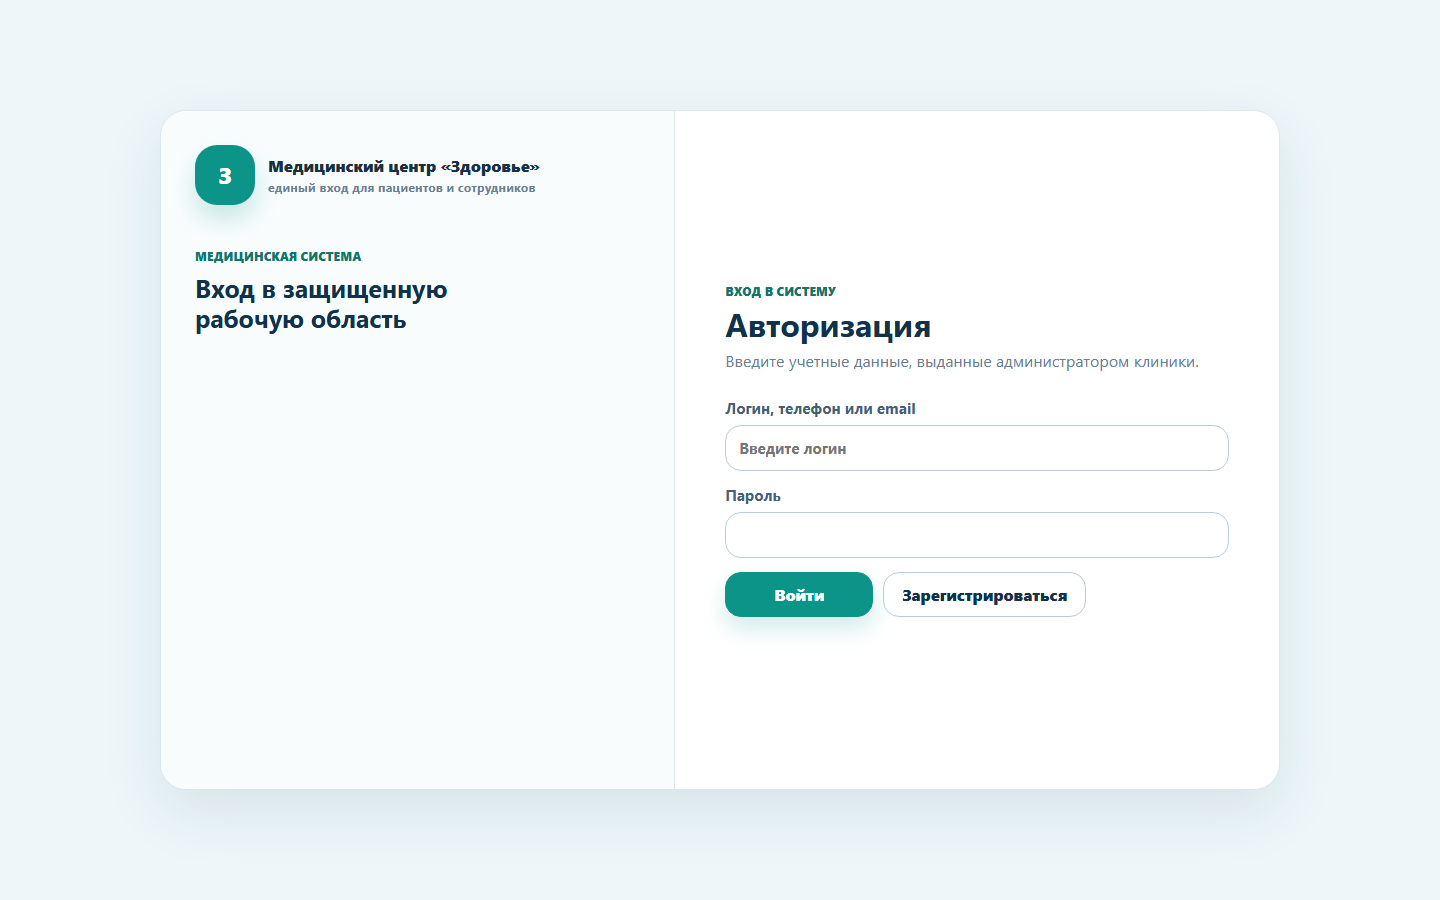
\includegraphics[width=\textwidth]{figures/frontend_login.png}
    \caption{Экран входа по пользователям}
    \label{fig:frontend-login}
\end{figure}

\begin{figure}[H]
    \centering
    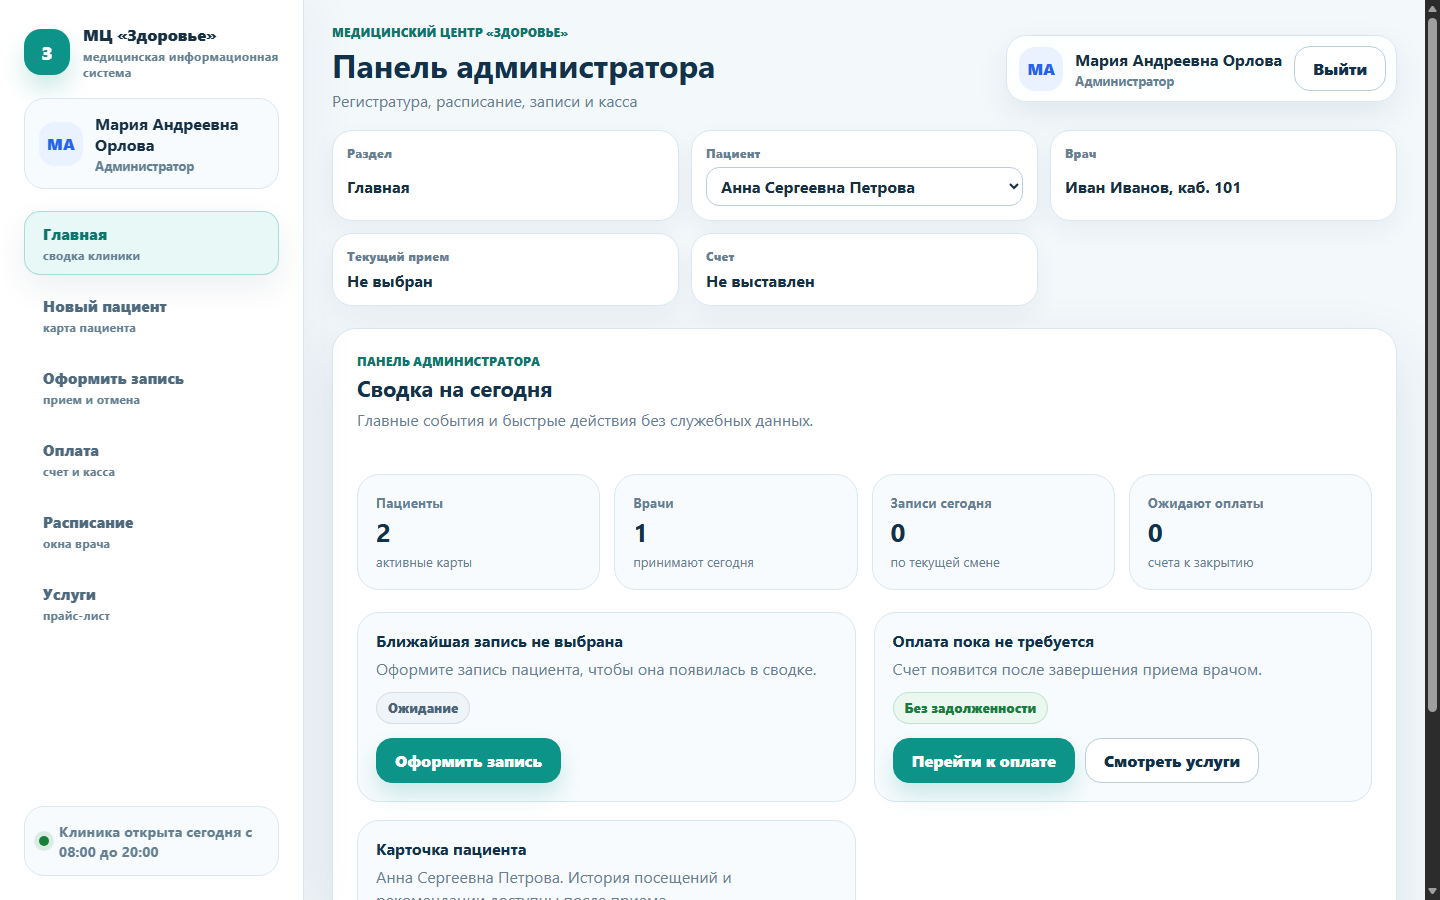
\includegraphics[width=\textwidth]{figures/frontend_role_workspace.png}
    \caption{Рабочее место пользователя после входа}
    \label{fig:frontend-workspace}
\end{figure}

\begin{figure}[H]
    \centering
    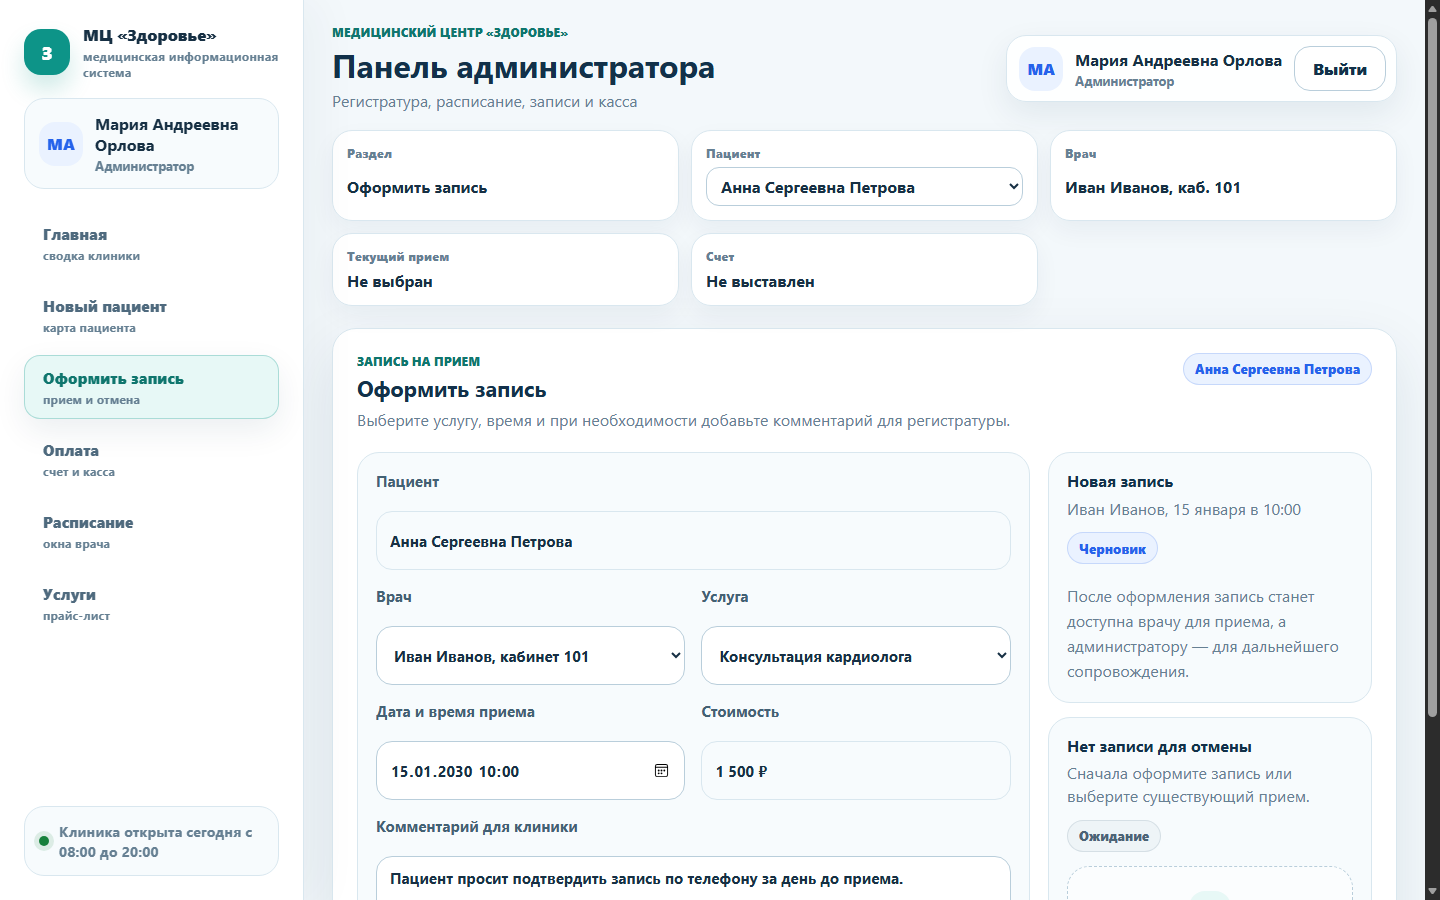
\includegraphics[width=\textwidth]{figures/frontend_workflow.png}
    \caption{Экран оформления записи на прием}
    \label{fig:frontend-workflow}
\end{figure}

Для входной валидации в Go используется пакет go-playground/validator. Входные UUID проверяются на ненулевое значение, телефон проверяется регулярным выражением, e-mail проверяется стандартным валидатором, а дата рождения передается типом, сериализуемым в формат YYYY-MM-DD. Фрагмент репозитория, вызывающего функции PostgreSQL через database/sql, приведен в листинге~\ref{lst:appendix-go-repository} приложения~А.

\section{Порядок тестирования и классы эквивалентности}

Тестирование выполнялось на трех уровнях: проверка входной валидации backend-приложения, проверка SQL-сценариев базы данных и проверка интеграционных сценариев через REST API. Для базы данных подготовлены сценарии функциональной проверки, конкурентного доступа и производительности.

Классы эквивалентности для функций базы данных приведены в таблице~\ref{tab:equivalence-classes}.

\begin{table}[H]
    \centering
    \caption{Классы эквивалентности для функций базы данных}
    \label{tab:equivalence-classes}
    \scriptsize
    \renewcommand{\arraystretch}{1.08}
    \begin{tabularx}{\textwidth}{|>{\raggedright\arraybackslash}p{3.5cm}|>{\raggedright\arraybackslash}X|>{\raggedright\arraybackslash}X|}
        \hline
        Функция & Корректные классы & Некорректные классы \tabularnewline
        \hline
        \begin{tabular}[t]{@{}l@{}}set\_\tabularnewline updated\_at\end{tabular} & Обновление строки таблицы, содержащей поле updated\_at. & Отсутствие поля updated\_at в таблице, к которой ошибочно подключен триггер. \tabularnewline
        \hline
        has\_role & Пользователь имеет требуемую роль; пользователь не имеет требуемую роль. & Несуществующий пользователь или несуществующий код роли. \tabularnewline
        \hline
        \begin{tabular}[t]{@{}l@{}}get\_service\_\tabularnewline price\end{tabular} & Для услуги найдена цена, действующая на заданный момент. & Услуга не имеет активной цены на заданный момент. \tabularnewline
        \hline
        \begin{tabular}[t]{@{}l@{}}book\_\tabularnewline appointment\end{tabular} & Активный пациент, активный врач, активная услуга, время в будущем, интервал входит в расписание и не пересекается с другой записью. & Прошедшее время, неактивный пациент, неактивный врач, услуга не закреплена за врачом, услуга неактивна, время вне расписания, отсутствие врача, пересечение с другой записью. \tabularnewline
        \hline
        \begin{tabular}[t]{@{}l@{}}cancel\_\tabularnewline appointment\end{tabular} & Отмена записи со статусом booked; отмена администратором; отмена пациентом более чем за 24 часа. & Несуществующая запись, статус не booked, отмена пациентом менее чем за 24 часа до приема. \tabularnewline
        \hline
        \begin{tabular}[t]{@{}l@{}}complete\_\tabularnewline visit\end{tabular} & Завершение записи врачом, связанным с приемом; завершение с базовой услугой; завершение с дополнительными оказанными услугами. & Несуществующая запись, другой врач, статус не booked, дополнительная услуга не закреплена за врачом. \tabularnewline
        \hline
        \begin{tabular}[t]{@{}l@{}}register\_\tabularnewline payment\end{tabular} & Регистрация оплаты с положительной суммой и допустимым способом оплаты. & Несуществующий счет, неположительная сумма, недопустимый способ оплаты. \tabularnewline
        \hline
        \begin{tabular}[t]{@{}l@{}}refresh\_\tabularnewline invoice\_state\end{tabular} & Нет оплат, частичная оплата, полная или избыточная оплата. & Несуществующий счет; некорректные строки счета невозможны при соблюдении ограничений CHECK. \tabularnewline
        \hline
        Триггеры пересчета счета & Добавление, изменение или удаление строки счета; добавление, изменение или удаление оплаты. & Ошибочная привязка триггера к таблице без поля invoice\_id. \tabularnewline
        \hline
    \end{tabularx}
\end{table}
\normalsize

Порядок проверки базы данных включает следующие шаги:
\begin{enumerate}
    \item создание структуры базы данных из сценария db/schema.sql;
    \item загрузку начальных данных из сценария db/seed.sql;
    \item выполнение сценария db/test\_scenarios.sql, проверяющего регистрацию пациента, валидацию e-mail и телефона, запись, запрет пересечения, отмену, проведение приема, формирование счета и оплату;
    \item выполнение двух сценариев конкурентного доступа:\\
    db/concurrency\_session\_1.sql;\\
    db/concurrency\_session\_2.sql;
    \item загрузку массового набора данных из db/bulk\_seed.sql и выполнение запросов EXPLAIN ANALYZE из db/performance.sql.
\end{enumerate}

Фрагмент сценария проверки некорректного класса эквивалентности для записи на прием приведен в листинге~\ref{lst:appendix-overlap-test} приложения~А.

На уровне backend выполняются unit-тесты валидаторов, обработки ошибок PostgreSQL, поведения кэша и HTTP-маршрутов. Для frontend выполняется сборка npm run build, подтверждающая корректность TypeScript-кода и клиентского интерфейса.

\section{Вывод}

В технологическом разделе обоснован выбор PostgreSQL, Redis, Go, Gin, React и TypeScript, описаны реализованные сущности, ограничения целостности, функции, триггеры, ролевая модель базы данных, REST-интерфейс доступа к данным и порядок тестирования. Реализация соответствует требованиям задания и использует возможности СУБД для контроля критических правил медицинской клиники.

\clearpage

% Исследовательский раздел
\chapter{Исследовательский раздел}

\section{Описание исследования}

В исследовательском разделе проведено исследование для оценки времени выполнения ключевых операций разработанной базы данных медицинской клиники при увеличении объема данных. Исследование выполнялось на контейнерном стенде, включающем PostgreSQL, Redis, backend-приложение на Go и frontend-приложение на React.

Для проведения исследования использовался сценарий research\_benchmark.sql из каталога db. В отличие от вспомогательных проверок, данный сценарий не откатывает изменения, а наполняет рабочую базу данных исследовательским набором записей. Это позволяет проводить замеры на реально заполненных таблицах, которые затем доступны backend-приложению и frontend-интерфейсу.

В ходе исследования последовательно формировались три серии данных: 5000, 20000 и 50000 записей в основных таблицах предметной области. После каждой серии выполнялась команда ANALYZE. Для исследования влияния индексов и оптимизации SQL-запросов выполнялись замеры внутри PostgreSQL: для каждой операции проводилось семь запусков EXPLAIN ANALYZE. В таблицах и графиках приведено среднее время выполнения в миллисекундах. Redis-кэширование исследовалось отдельно как полное время HTTP-запроса к backend-приложению.

Измерялись следующие операции:
\begin{itemize}
    \item получение расписания врача за период с использованием индексов;
    \item получение расписания врача при отключенных index scan и bitmap scan;
    \item получение расписания врача через backend при последовательном добавлении индексов и Redis-кэширования;
    \item получение истории приемов пациента;
    \item получение счетов пациента;
    \item построение отчета по выручке врача;
    \item вставка новой записи на прием через функцию book\_appointment схемы scheduling;
    \item поиск строк по идентификатору пациента с индексом и без индекса на отдельной исследовательской таблице.
\end{itemize}

После завершения исследования база данных содержала строки, приведенные в таблице~\ref{tab:research-final-counts}.

\begin{table}[H]
    \centering
    \caption{Количество строк после выполнения исследовательского сценария}
    \label{tab:research-final-counts}
    \footnotesize
    \renewcommand{\arraystretch}{1.08}
    \begin{tabularx}{\textwidth}{|>{\raggedright\arraybackslash}p{7cm}|>{\centering\arraybackslash}X|}
        \hline
        Таблица & Количество строк \tabularnewline
        \hline
        medical.patients & 50002 \tabularnewline
        \hline
        scheduling.appointments & 50008 \tabularnewline
        \hline
        medical.visits & 50000 \tabularnewline
        \hline
        billing.invoices & 50000 \tabularnewline
        \hline
        billing.invoice\_items & 50000 \tabularnewline
        \hline
        billing.payments & 50000 \tabularnewline
        \hline
    \end{tabularx}
\end{table}
\normalsize

\section{Результаты исследования}

Результаты PostgreSQL-замеров приведены в таблице~\ref{tab:research-results}. Время измерялось в миллисекундах.

\begin{table}[H]
    \centering
    \caption{Среднее время выполнения операций}
    \label{tab:research-results}
    \scriptsize
    \renewcommand{\arraystretch}{1.08}
    \begin{tabularx}{\textwidth}{|>{\centering\arraybackslash}p{1.75cm}|>{\centering\arraybackslash}p{1.9cm}|>{\centering\arraybackslash}p{2.45cm}|>{\centering\arraybackslash}p{1.75cm}|>{\centering\arraybackslash}p{1.65cm}|>{\centering\arraybackslash}p{1.65cm}|>{\centering\arraybackslash}X|}
        \hline
        Объем & Расписание & Расписание без index scan & История пациента & Счета пациента & Отчет & Запись \tabularnewline
        \hline
        5000 & 1,717 & 1,745 & 0,176 & 0,129 & 4,828 & 0,559 \tabularnewline
        \hline
        20000 & 3,387 & 6,292 & 0,194 & 0,403 & 19,865 & 0,253 \tabularnewline
        \hline
        50000 & 7,614 & 23,188 & 0,143 & 1,325 & 57,672 & 0,276 \tabularnewline
        \hline
    \end{tabularx}
\end{table}
\normalsize

График времени выполнения операций чтения приведен на рисунке~\ref{fig:research-read-operations}.

\begin{figure}[H]
    \centering
    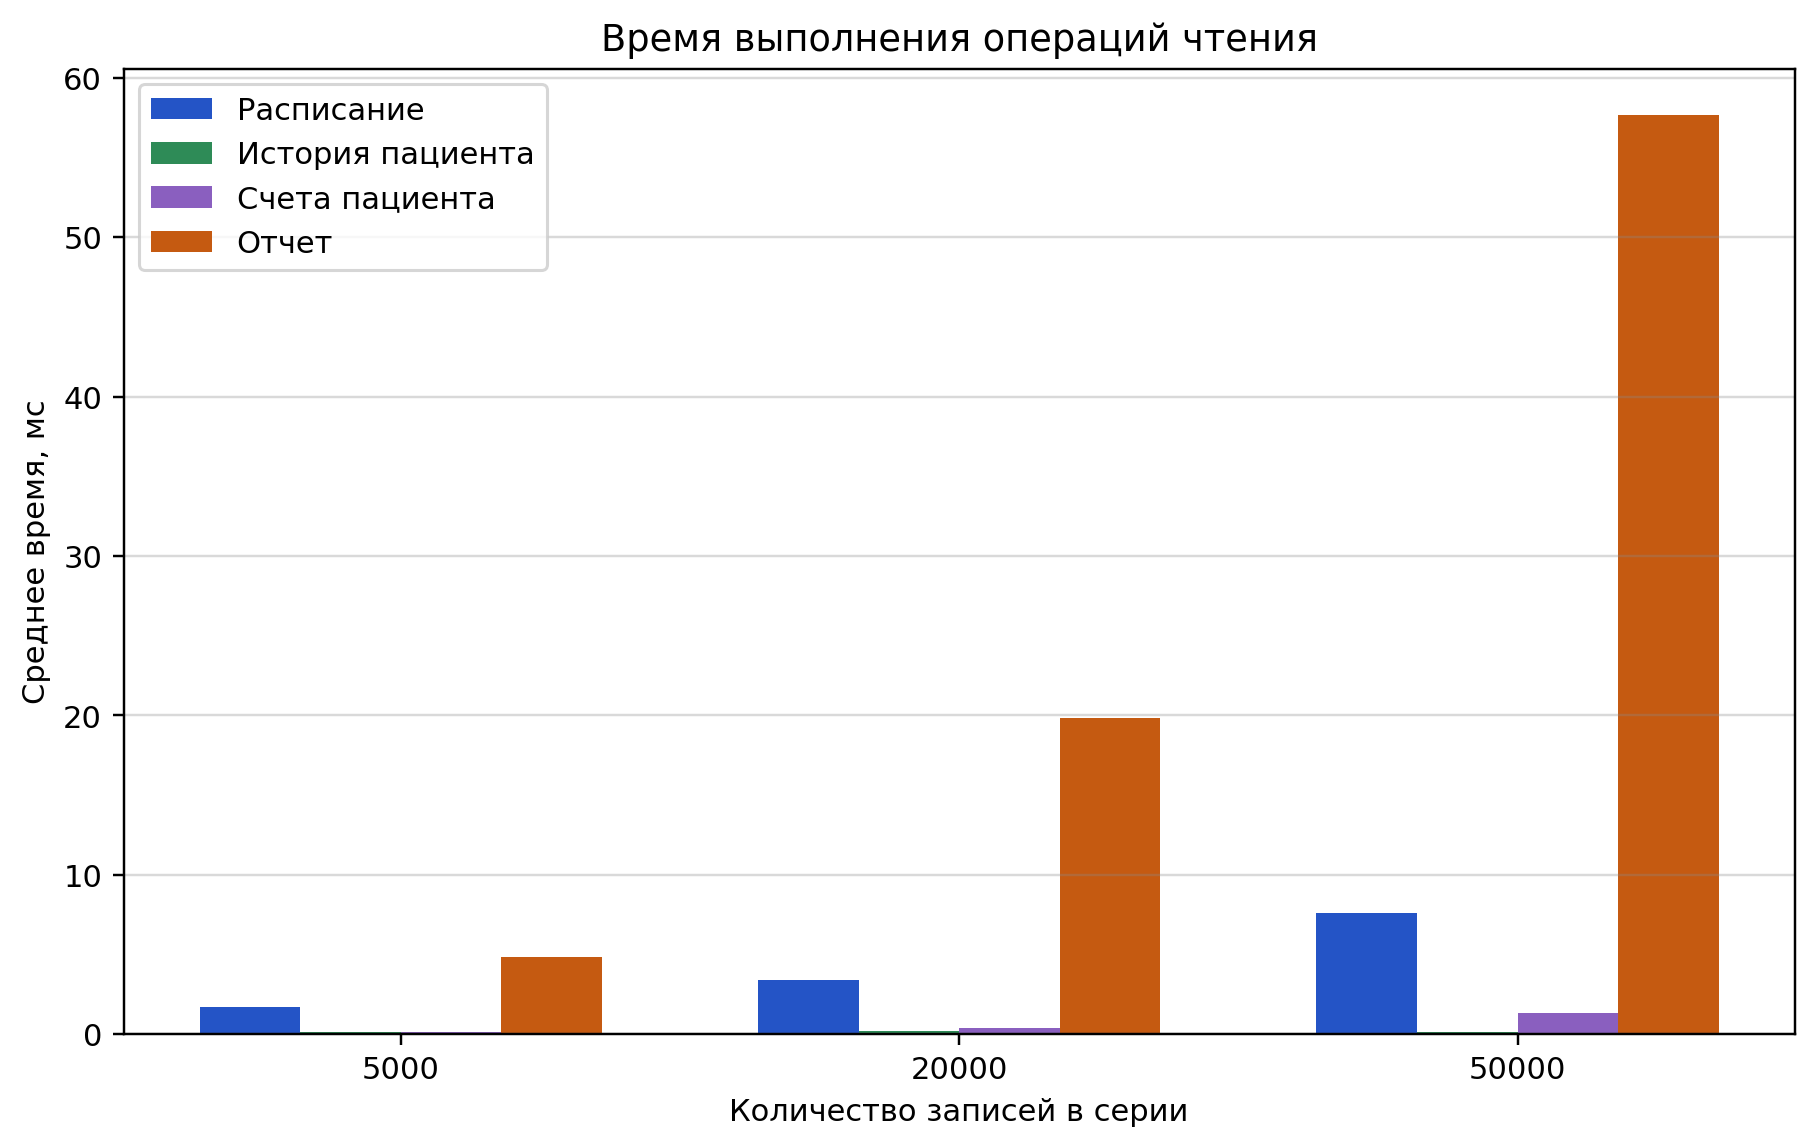
\includegraphics[width=0.95\textwidth]{figures/research_read_operations.png}
    \caption{Время выполнения операций чтения при разном объеме данных}
    \label{fig:research-read-operations}
\end{figure}

На рисунке~\ref{fig:research-index-impact} показано сравнение получения расписания врача при обычном плане выполнения и при отключенных index scan и bitmap scan.

\begin{figure}[H]
    \centering
    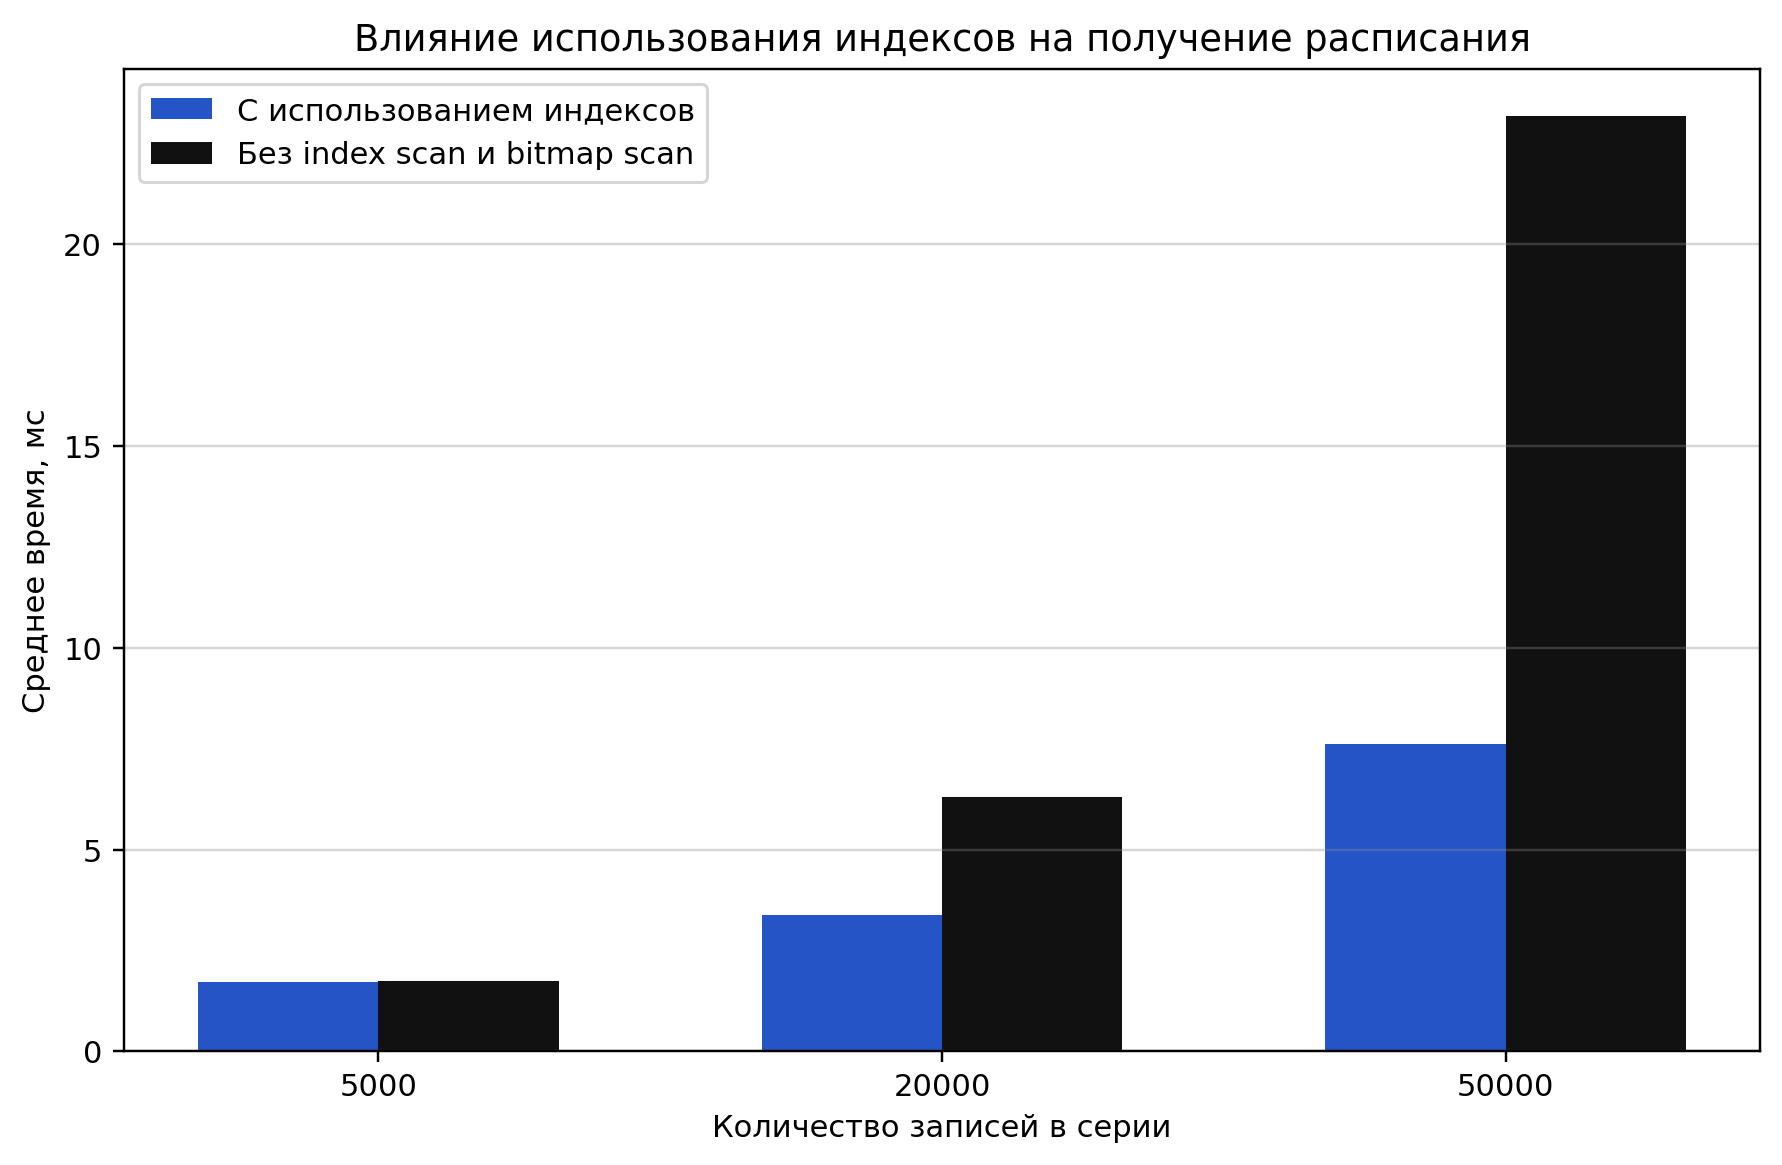
\includegraphics[width=0.9\textwidth]{figures/research_index_impact.png}
    \caption{Влияние использования индексов на получение расписания врача}
    \label{fig:research-index-impact}
\end{figure}

Дополнительно были выполнены замеры последовательного ускорения получения расписания врача на уровне полного HTTP-запроса к backend-приложению. Такой замер позволяет сравнить не только время выполнения SQL-запроса внутри PostgreSQL, но и полный путь пользовательского запроса: HTTP-обработку, обращение к базе данных или Redis, сериализацию JSON и передачу ответа.

Для каждого объема данных сравнивались три режима: запрос без Redis-кэша и без обычных B-tree индексов расписания, запрос без Redis-кэша при наличии индексов и повторный запрос из Redis-кэша. Перед запросами без Redis выполнялась очистка ключей Redis, чтобы backend был вынужден читать данные из PostgreSQL. Для режима без индексов временно удалялись индексы \texttt{idx\_schedule\_availability\_lookup}, \texttt{idx\_schedule\_absence\_lookup} и \texttt{idx\_appointments\_doctor\_time}; после замеров индексы создавались обратно. Для каждого режима усреднялись семь запусков. Результаты приведены в таблице~\ref{tab:research-http-schedule-chain}.

\begin{table}[H]
    \centering
    \caption{Ускорение полного HTTP-запроса расписания врача}
    \label{tab:research-http-schedule-chain}
    \scriptsize
    \renewcommand{\arraystretch}{1.08}
    \begin{tabularx}{\textwidth}{|>{\centering\arraybackslash}p{1.25cm}|>{\centering\arraybackslash}p{1.7cm}|>{\centering\arraybackslash}p{1.7cm}|>{\centering\arraybackslash}p{1.7cm}|>{\centering\arraybackslash}p{1.55cm}|>{\centering\arraybackslash}p{1.35cm}|>{\centering\arraybackslash}X|}
        \hline
        Объем & Без инд., мс & С инд., мс & Redis hit, мс & Индексы, \% & Redis, \% & Итог, \% \tabularnewline
        \hline
        5000 & 36,893 & 29,719 & 26,801 & 19,44 & 9,82 & 27,35 \tabularnewline
        \hline
        20000 & 149,756 & 105,388 & 97,442 & 29,63 & 7,54 & 34,93 \tabularnewline
        \hline
        50000 & 292,108 & 279,806 & 260,563 & 4,21 & 6,88 & 10,80 \tabularnewline
        \hline
    \end{tabularx}
\end{table}
\normalsize

На рисунке~\ref{fig:research-http-schedule-chain} показана цепочка ускорения полного HTTP-запроса: сначала за счет индексов PostgreSQL, затем за счет Redis-кэширования повторного запроса.

\begin{figure}[H]
    \centering
    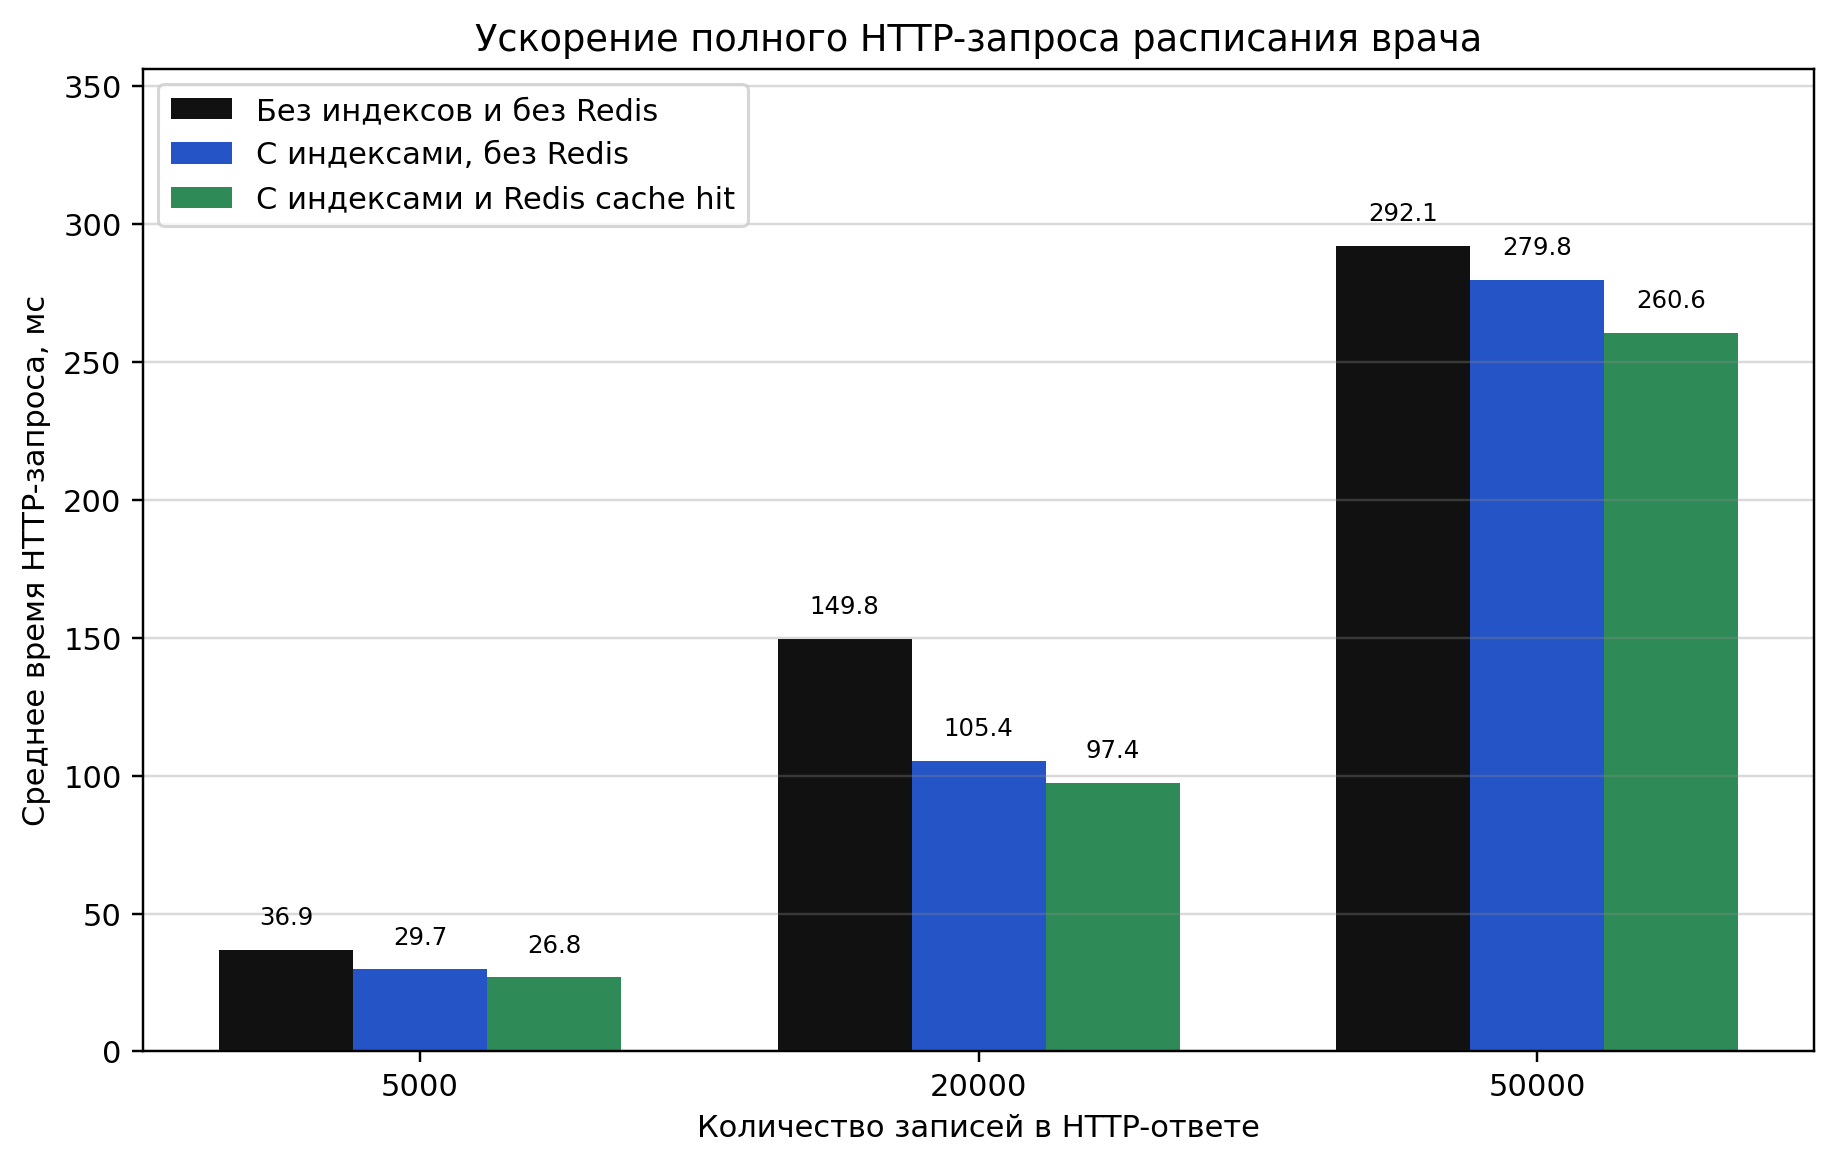
\includegraphics[width=0.9\textwidth]{figures/research_http_schedule_chain.png}
    \caption{Ускорение полного HTTP-запроса расписания врача}
    \label{fig:research-http-schedule-chain}
\end{figure}

График времени вставки новой записи на прием приведен на рисунке~\ref{fig:research-book-appointment}.

\begin{figure}[H]
    \centering
    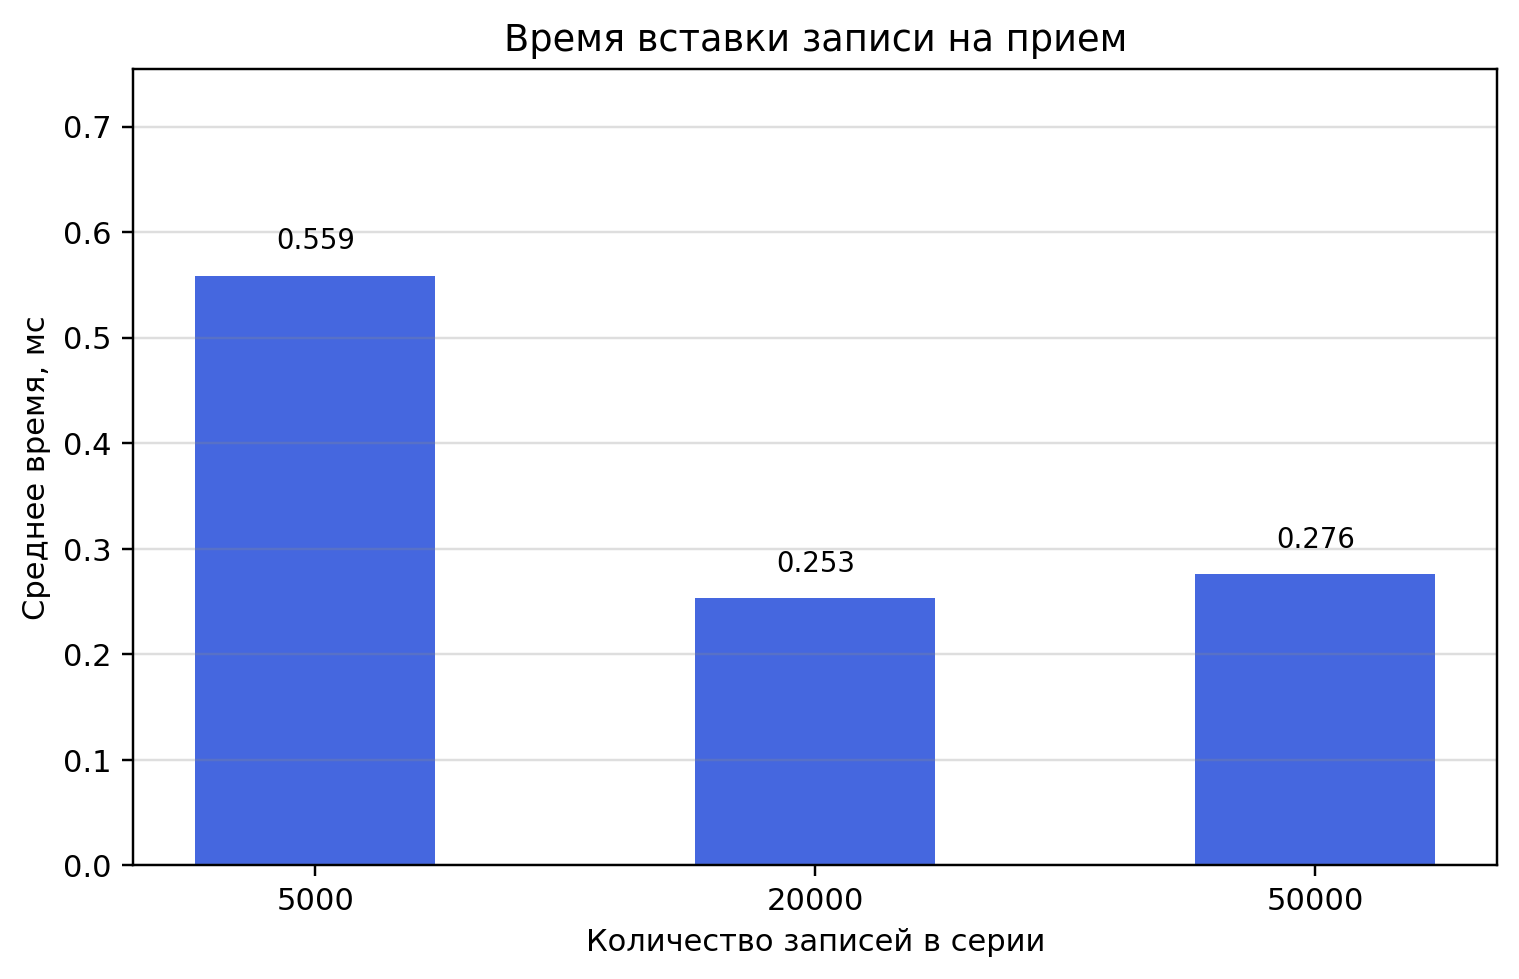
\includegraphics[width=0.86\textwidth]{figures/research_book_appointment.png}
    \caption{Время вставки записи на прием при разном объеме данных}
    \label{fig:research-book-appointment}
\end{figure}

Дополнительное исследование влияния индекса на поиск строк по идентификатору пациента приведено на рисунке~\ref{fig:research-index-search-piecewise}. Для него использовалась отдельная таблица \texttt{research\_index\_search}, которая последовательно наполнялась наборами от 1000 до 50000 строк. После каждого наполнения сравнивалось выполнение запроса без индекса и с B-tree индексом по полю \texttt{patient\_id}; для каждой точки усреднялись пять запусков EXPLAIN ANALYZE.

\begin{figure}[H]
    \centering
    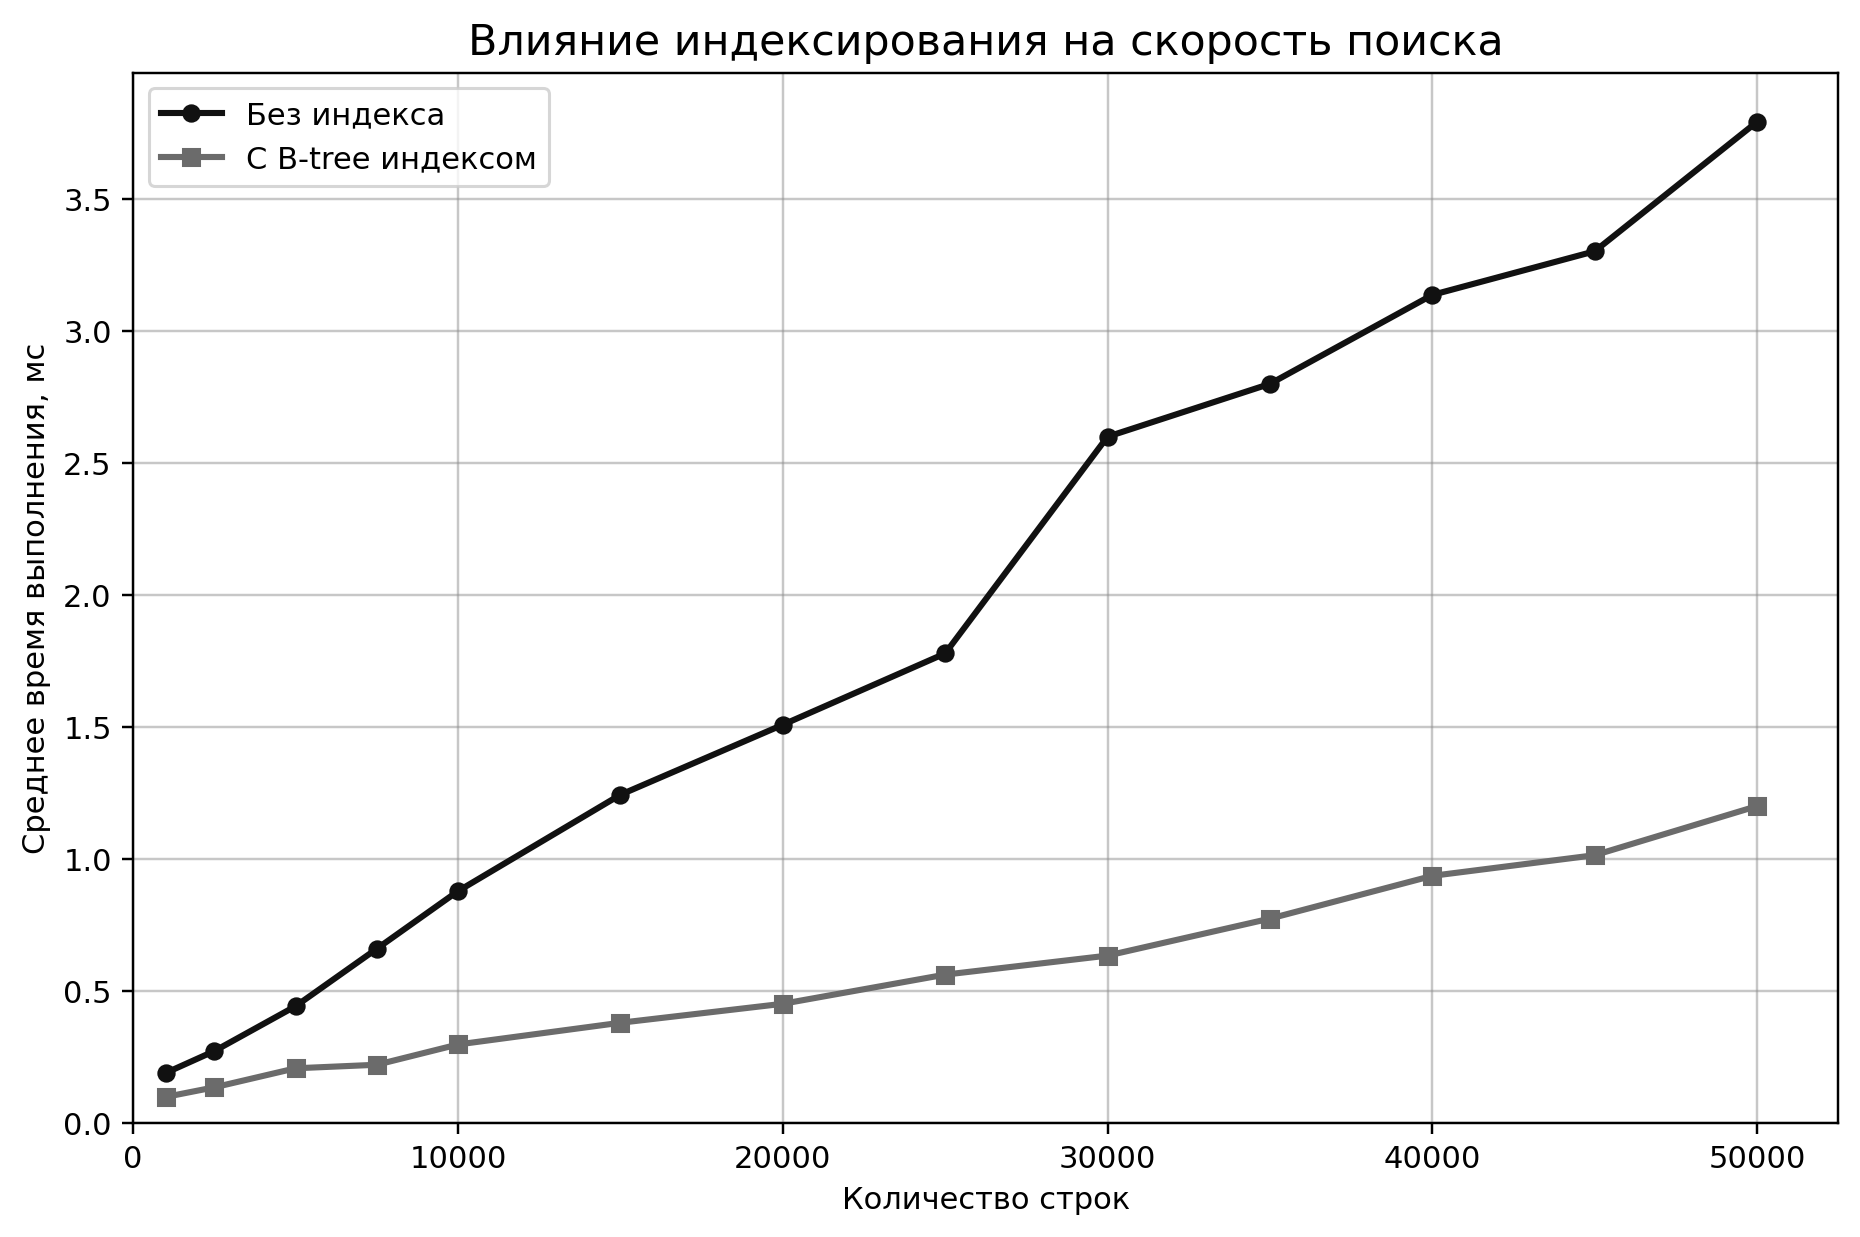
\includegraphics[width=0.9\textwidth]{figures/research_index_search_piecewise.png}
    \caption{Влияние индексирования на поиск по идентификатору пациента}
    \label{fig:research-index-search-piecewise}
\end{figure}

\section{Анализ результатов}

Наибольшее время выполнения показал отчет по выручке врача. При увеличении объема данных с 5000 до 50000 записей среднее время построения отчета выросло с 4,828 мс до 57,672 мс. Это объясняется тем, что запрос соединяет таблицы записей, приемов и счетов, после чего выполняет группировку результата.

Получение расписания врача при использовании индексов заняло 7,614 мс на объеме 50000 записей. При отключенных index scan и bitmap scan время той же операции выросло до 23,188 мс. Таким образом, на максимальном исследованном объеме использование индексов ускорило получение расписания примерно в 3 раза.

Дополнительный HTTP-замер показывает последовательный эффект оптимизаций на уровне всего backend-запроса. На объеме 20000 записей добавление индексов уменьшило среднее время с 149,756 мс до 105,388 мс, то есть на 29,63\%. Повторное чтение из Redis-кэша уменьшило время до 97,442 мс. На объеме 50000 записей итоговый выигрыш составил 10,80\%: время снизилось с 292,108 мс до 260,563 мс. Меньший выигрыш на максимальном объеме связан с тем, что существенную часть полного HTTP-запроса занимает не только доступ к PostgreSQL, но и сериализация, десериализация и передача большого JSON-ответа.

Запрос истории пациента и запрос счетов пациента выполнялись быстрее агрегирующего отчета. Для истории пациента среднее время на максимальном объеме составило 0,143 мс, для счетов пациента --- 1,325 мс. Это связано с тем, что данные запросы используют условия по patient\_id и ограничение количества возвращаемых строк.

Вставка записи через функцию scheduling.book\_appointment оставалась устойчивой на всех исследованных объемах. На 50000 записей среднее время составило 0,276 мс. Небольшая немонотонность значений связана с тем, что измерения выполняются на долях миллисекунды и зависят от состояния кэша PostgreSQL и планировщика контейнера. Кроме того, функция не просматривает всю таблицу записей, а выполняет проверки активности пациента, врача, услуги, доступности врача и отсутствия пересечения по времени с опорой на индексы и ограничение EXCLUDE.

Дополнительный график поиска по \texttt{patient\_id} показывает, что при росте числа строк запрос без индекса становится заметно медленнее, тогда как запрос с B-tree индексом растет значительно слабее. На объеме 50000 строк среднее время поиска без индекса составило 3,792 мс, а с индексом --- 1,201 мс.

\section{Вывод}

В результате исследования установлено, что разработанная структура базы данных сохраняет приемлемое время выполнения ключевых операций на объеме 50000 записей в основных таблицах. Наиболее чувствительной к росту объема данных является операция построения отчета по выручке, так как она требует соединения и агрегации большого числа строк.

Использование индексов существенно влияет на операции расписания: при 50000 записей отключение index scan увеличило время получения расписания с 7,614 мс до 23,188 мс. Дополнительный замер поиска по \texttt{patient\_id} также показал преимущество индексированного доступа. Операция записи пациента на прием через функцию базы данных осталась в пределах 0,276 мс на максимальном объеме, что подтверждает корректность выбранной стратегии согласованности: транзакционная функция PostgreSQL, индексы и EXCLUDE-ограничение позволяют предотвращать конфликтующие записи без существенного роста времени вставки.

Дополнительное исследование полного HTTP-запроса показало, что последовательное добавление индексов и Redis-кэширования уменьшает время получения расписания врача. При этом величина выигрыша зависит от размера ответа: на больших объемах данных ограничивающим фактором становится не только доступ к PostgreSQL, но и сериализация результата. Поэтому Redis целесообразно использовать для часто повторяющихся запросов расписания и прайс-листа, а также совместно с ограничением размера возвращаемого периода.

\clearpage

% Заключение
\chapter*{ЗАКЛЮЧЕНИЕ}
\addcontentsline{toc}{chapter}{ЗАКЛЮЧЕНИЕ}

В ходе выполнения курсовой работы достигнута поставленная цель: спроектированы и реализованы база данных медицинской клиники и приложение доступа к ней, обеспечивающие корректную запись на прием, проведение приема, формирование счетов, учет оплат и кэширование часто используемых данных.

При выполнении работы получены следующие основные результаты:
\begin{enumerate}
    \item проведен анализ предметной области медицинской клиники и формализована задача разработки базы данных и приложения;
    \item спроектированы сущности базы данных, связи между ними, ограничения целостности, ролевая модель, процедуры и триггеры;
    \item выбраны средства реализации, соответствующие требованиям задания: PostgreSQL, Redis, Go, Gin, React и TypeScript;
    \item реализованы таблицы, индексы, домены, перечислимые типы, хранимые процедуры, триггеры и прикладной REST API;
    \item разработаны тестовые сценарии для проверки записи, отмены, проведения приема, формирования счетов и регистрации оплаты;
    \item исследованы конкурентный доступ и влияние индексов на производительность ключевых операций.
\end{enumerate}

Поставленные задачи решены в полном объеме: разработаны структура базы данных, ролевая модель, функции, триггеры, REST API, frontend-интерфейс и внешнее кэширование с использованием Redis.

Практическая проверка показала, что система запрещает конфликтующие записи по времени, корректно выполняет основные бизнес-операции и ускоряет чтение расписания и прайс-листа за счет кэширования. Результаты исследования подтвердили приемлемое время выполнения ключевых операций на выбранных объемах данных.

Разработанная система может использоваться как основа информационной системы небольшого медицинского центра. Для дальнейшего развития рекомендуется добавить журнал аудита действий пользователей, расширить управление расписанием нескольких врачей и реализовать резервное копирование базы данных.

\clearpage

% Список использованных источников
\phantomsection
\renewcommand{\bibname}{СПИСОК ИСПОЛЬЗОВАННЫХ ИСТОЧНИКОВ}
\addcontentsline{toc}{chapter}{СПИСОК ИСПОЛЬЗОВАННЫХ ИСТОЧНИКОВ}

\begin{thebibliography}{99}
    \bibitem{date_intro}
    Дейт~К.\,Дж. Введение в системы баз данных~/ К.\,Дж.~Дейт. --- 8-е изд. --- М.\,: Вильямс, 2005. --- 1328~с.

    \bibitem{connolly_db}
    Коннолли~Т. Базы данных: проектирование, реализация и сопровождение. Теория и практика~/ Т.~Коннолли, К.~Бегг. --- 3-е изд. --- М.\,: Вильямс, 2003. --- 1436~с.

    \bibitem{postgres_main}
    PostgreSQL: Documentation [Электронный ресурс]. --- URL: \url{https://www.postgresql.org/docs/} (дата обращения: 01.04.2026).

    \bibitem{postgres_range}
    PostgreSQL: Range Types [Электронный ресурс]. --- URL: \url{https://www.postgresql.org/docs/current/rangetypes.html} (дата обращения: 01.04.2026).

    \bibitem{postgres_constraints}
    PostgreSQL: Exclusion Constraints [Электронный ресурс]. --- URL: \url{https://www.postgresql.org/docs/current/ddl-constraints.html} (дата обращения: 01.04.2026).

    \bibitem{redis_docs}
    Redis: Documentation [Электронный ресурс]. --- URL: \url{https://redis.io/docs/latest/} (дата обращения: 01.04.2026).

    \bibitem{go_docs}
    Go: Documentation [Электронный ресурс]. --- URL: \url{https://go.dev/doc/} (дата обращения: 01.04.2026).

    \bibitem{gin_docs}
    Gin Web Framework: Documentation [Электронный ресурс]. --- URL: \url{https://gin-gonic.com/} (дата обращения: 01.04.2026).

    \bibitem{react_docs}
    React: Documentation [Электронный ресурс]. --- URL: \url{https://react.dev/} (дата обращения: 01.04.2026).

    \bibitem{typescript_docs}
    TypeScript: Documentation [Электронный ресурс]. --- URL: \url{https://www.typescriptlang.org/docs/} (дата обращения: 01.04.2026).
\end{thebibliography}

\clearpage

% Приложения
\appendix

\clearpage
\phantomsection
\chapter*{ПРИЛОЖЕНИЕ А}
\addcontentsline{toc}{chapter}{ПРИЛОЖЕНИЕ А}
\renewcommand{\thelstlisting}{А.\arabic{lstlisting}}
\setcounter{lstlisting}{0}

\begin{lstlisting}[language=SQL,caption={Фрагмент реализации сущности записи на прием},label={lst:appendix-appointments}]
CREATE TABLE IF NOT EXISTS scheduling.appointments (
    id UUID PRIMARY KEY DEFAULT gen_random_uuid(),
    patient_id UUID NOT NULL REFERENCES medical.patients(id) ON DELETE RESTRICT,
    doctor_id UUID NOT NULL REFERENCES medical.doctors(id) ON DELETE RESTRICT,
    booked_service_id UUID NOT NULL REFERENCES catalog.services(id) ON DELETE RESTRICT,
    starts_at TIMESTAMPTZ NOT NULL,
    ends_at TIMESTAMPTZ NOT NULL,
    status scheduling.appointment_status NOT NULL DEFAULT 'booked',
    note TEXT,
    cancellation_reason TEXT,
    created_by_user_id UUID NOT NULL REFERENCES security.users(id) ON DELETE RESTRICT,
    cancelled_by_user_id UUID REFERENCES security.users(id) ON DELETE RESTRICT,
    completed_at TIMESTAMPTZ,
    created_at TIMESTAMPTZ NOT NULL DEFAULT NOW(),
    updated_at TIMESTAMPTZ NOT NULL DEFAULT NOW(),
    period TSTZRANGE GENERATED ALWAYS AS (tstzrange(starts_at, ends_at, '[)')) STORED,
    CHECK (ends_at > starts_at)
);
\end{lstlisting}

\begin{lstlisting}[language=SQL,caption={Фрагменты реализации ограничений целостности},label={lst:appendix-constraints}]
CREATE DOMAIN security.email_address AS VARCHAR(150)
    CHECK (VALUE IS NULL OR VALUE ~* '^[A-Z0-9._%+-]+@[A-Z0-9.-]+\.[A-Z]{2,}$');

CREATE DOMAIN security.phone_number AS VARCHAR(20)
    CHECK (VALUE IS NULL OR VALUE ~ '^\+?[1-9][0-9]{10,14}$');

ALTER TABLE catalog.service_prices
    ADD CONSTRAINT service_prices_no_overlap
    EXCLUDE USING gist (service_id WITH =, period WITH &&);

ALTER TABLE scheduling.doctor_availability
    ADD CONSTRAINT doctor_availability_no_overlap
    EXCLUDE USING gist (doctor_id WITH =, period WITH &&)
    WHERE (is_active);

ALTER TABLE scheduling.appointments
    ADD CONSTRAINT appointments_doctor_no_overlap
    EXCLUDE USING gist (doctor_id WITH =, period WITH &&)
    WHERE (status IN ('booked', 'completed'));
\end{lstlisting}

\begin{lstlisting}[language=SQL,caption={Функция получения актуальной цены услуги},label={lst:appendix-get-service-price}]
CREATE OR REPLACE FUNCTION catalog.get_service_price(
    p_service_id UUID,
    p_at TIMESTAMPTZ
)
RETURNS NUMERIC(12,2)
LANGUAGE plpgsql
AS $$
DECLARE
    v_price NUMERIC(12,2);
BEGIN
    SELECT sp.price
      INTO v_price
      FROM catalog.service_prices sp
     WHERE sp.service_id = p_service_id
       AND sp.effective_from <= p_at
       AND (sp.effective_to IS NULL OR sp.effective_to > p_at)
     ORDER BY sp.effective_from DESC
     LIMIT 1;

    IF v_price IS NULL THEN
        RAISE EXCEPTION USING ERRCODE = '22023',
            MESSAGE = format('Price is not found for service %s at %s',
                             p_service_id,
                             p_at);
    END IF;

    RETURN v_price;
END;
$$;
\end{lstlisting}

\begin{lstlisting}[language=SQL,caption={Фрагмент функции записи на прием},label={lst:appendix-book-appointment}]
CREATE OR REPLACE FUNCTION scheduling.book_appointment(
    p_patient_id UUID,
    p_doctor_id UUID,
    p_service_id UUID,
    p_starts_at TIMESTAMPTZ,
    p_created_by_user_id UUID,
    p_note TEXT DEFAULT NULL
)
RETURNS UUID
LANGUAGE plpgsql
AS $$
DECLARE
    v_duration INTEGER;
    v_ends_at TIMESTAMPTZ;
    v_appointment_id UUID;
BEGIN
    IF p_starts_at <= NOW() THEN
        RAISE EXCEPTION USING ERRCODE = '22023',
            MESSAGE = 'Appointment start time must be in the future';
    END IF;

    IF NOT EXISTS (
        SELECT 1 FROM medical.patients
         WHERE id = p_patient_id
           AND status = 'active'
    ) THEN
        RAISE EXCEPTION USING ERRCODE = '22023',
            MESSAGE = format('Patient %s is inactive', p_patient_id);
    END IF;

    IF NOT EXISTS (
        SELECT 1 FROM medical.doctors
         WHERE id = p_doctor_id
           AND status = 'active'
    ) THEN
        RAISE EXCEPTION USING ERRCODE = '22023',
            MESSAGE = format('Doctor %s is inactive', p_doctor_id);
    END IF;

    IF NOT EXISTS (
        SELECT 1
          FROM medical.doctor_services
         WHERE doctor_id = p_doctor_id
           AND service_id = p_service_id
    ) THEN
        RAISE EXCEPTION USING ERRCODE = '22023',
            MESSAGE = format('Service %s is not assigned to doctor %s',
                             p_service_id,
                             p_doctor_id);
    END IF;

    SELECT duration_minutes
      INTO v_duration
      FROM catalog.services
     WHERE id = p_service_id
       AND status = 'active';

    IF v_duration IS NULL THEN
        RAISE EXCEPTION USING ERRCODE = '22023',
            MESSAGE = format('Service %s is inactive', p_service_id);
    END IF;

    v_ends_at := p_starts_at + make_interval(mins => v_duration);

    IF NOT EXISTS (
        SELECT 1
          FROM scheduling.doctor_availability da
         WHERE da.doctor_id = p_doctor_id
           AND da.is_active
           AND da.starts_at <= p_starts_at
           AND da.ends_at >= v_ends_at
    ) THEN
        RAISE EXCEPTION USING ERRCODE = '22023',
            MESSAGE = 'Time is outside doctor availability';
    END IF;

    INSERT INTO scheduling.appointments (
        patient_id,
        doctor_id,
        booked_service_id,
        starts_at,
        ends_at,
        status,
        note,
        created_by_user_id
    )
    VALUES (
        p_patient_id,
        p_doctor_id,
        p_service_id,
        p_starts_at,
        v_ends_at,
        'booked',
        p_note,
        p_created_by_user_id
    )
    RETURNING id INTO v_appointment_id;

    RETURN v_appointment_id;
END;
$$;
\end{lstlisting}

\begin{lstlisting}[language=SQL,caption={Триггеры пересчета состояния счета},label={lst:appendix-refresh-invoice-triggers}]
CREATE OR REPLACE FUNCTION billing.trg_refresh_invoice_from_items()
RETURNS trigger
LANGUAGE plpgsql
AS $$
BEGIN
    PERFORM billing.refresh_invoice_state(COALESCE(NEW.invoice_id, OLD.invoice_id));
    RETURN COALESCE(NEW, OLD);
END;
$$;

CREATE TRIGGER trg_invoice_items_refresh_invoice
AFTER INSERT OR UPDATE OR DELETE ON billing.invoice_items
FOR EACH ROW
EXECUTE FUNCTION billing.trg_refresh_invoice_from_items();

CREATE TRIGGER trg_payments_refresh_invoice
AFTER INSERT OR UPDATE OR DELETE ON billing.payments
FOR EACH ROW
EXECUTE FUNCTION billing.trg_refresh_invoice_from_payments();
\end{lstlisting}

\begin{lstlisting}[language=SQL,caption={Реализация ролей базы данных},label={lst:appendix-db-roles}]
DO $$
BEGIN
    IF NOT EXISTS (SELECT 1 FROM pg_roles WHERE rolname = 'clinic_owner') THEN
        CREATE ROLE clinic_owner NOLOGIN;
    END IF;

    IF NOT EXISTS (SELECT 1 FROM pg_roles WHERE rolname = 'clinic_api') THEN
        CREATE ROLE clinic_api NOLOGIN;
    END IF;

    IF NOT EXISTS (SELECT 1 FROM pg_roles WHERE rolname = 'clinic_reporting') THEN
        CREATE ROLE clinic_reporting NOLOGIN;
    END IF;
END
$$;

GRANT USAGE ON SCHEMA security, catalog, medical, scheduling, billing
TO clinic_api, clinic_reporting;

GRANT SELECT, INSERT, UPDATE, DELETE ON ALL TABLES
IN SCHEMA security, catalog, medical, scheduling, billing
TO clinic_api;

GRANT EXECUTE ON ALL FUNCTIONS
IN SCHEMA security, catalog, medical, scheduling, billing
TO clinic_api;

GRANT SELECT ON ALL TABLES
IN SCHEMA security, catalog, medical, scheduling, billing
TO clinic_reporting;
\end{lstlisting}

\begin{lstlisting}[language=Go,caption={Вызов функций PostgreSQL из репозитория},label={lst:appendix-go-repository}]
func (r *AppointmentRepository) Book(
    ctx context.Context,
    command model.BookAppointmentCommand,
) (uuid.UUID, error) {
    var appointmentID uuid.UUID
    const query = "SELECT scheduling.book_appointment($1, $2, $3, " +
        "$4, $5, $6)"
    err := r.db.QueryRowContext(ctx, query,
        command.PatientID,
        command.DoctorID,
        command.ServiceID,
        command.StartsAt,
        command.CreatedByUserID,
        nullableString(command.Note),
    ).Scan(&appointmentID)

    return appointmentID, err
}

func (r *AppointmentRepository) RegisterPayment(
    ctx context.Context,
    command model.RegisterPaymentCommand,
) (uuid.UUID, error) {
    var paymentID uuid.UUID
    const query = "SELECT billing.register_payment($1, $2, $3, $4, $5)"
    err := r.db.QueryRowContext(ctx, query,
        command.InvoiceID,
        command.Amount,
        string(command.PaymentMethod),
        command.ReceivedByUserID,
        nullableString(command.ExternalReference),
    ).Scan(&paymentID)

    return paymentID, err
}
\end{lstlisting}

\begin{lstlisting}[language=SQL,caption={Проверка запрета пересечения записей},label={lst:appendix-overlap-test}]
BEGIN
    PERFORM scheduling.book_appointment(
        v_patient_2,
        v_doctor,
        v_service_consult,
        TIMESTAMPTZ '2030-01-15 10:15:00+03',
        v_patient_user,
        'SCENARIO_OVERLAP_REJECT'
    );
    v_rejected := FALSE;
EXCEPTION WHEN OTHERS THEN
    v_rejected := TRUE;
END;

IF NOT v_rejected THEN
    RAISE EXCEPTION 'Overlapping booking was not rejected';
END IF;
\end{lstlisting}

К расчётно-пояснительной записке курсовой работы прилагаются следующие материалы:
\begin{itemize}
    \item презентация к курсовой работе, состоящая из 21 слайда;
    \item USB-флеш-накопитель с исходными кодами, электронными версиями РПЗ и презентации.
\end{itemize}

\clearpage


\end{document}
